\documentclass[twoside]{book}

% Packages required by doxygen
\usepackage{fixltx2e}
\usepackage{calc}
\usepackage{doxygen}
\usepackage[export]{adjustbox} % also loads graphicx
\usepackage{graphicx}
\usepackage[utf8]{inputenc}
\usepackage{makeidx}
\usepackage{multicol}
\usepackage{multirow}
\PassOptionsToPackage{warn}{textcomp}
\usepackage{textcomp}
\usepackage[nointegrals]{wasysym}
\usepackage[table]{xcolor}

% Font selection
\usepackage[T1]{fontenc}
\usepackage[scaled=.90]{helvet}
\usepackage{courier}
\usepackage{amssymb}
\usepackage{sectsty}
\renewcommand{\familydefault}{\sfdefault}
\allsectionsfont{%
  \fontseries{bc}\selectfont%
  \color{darkgray}%
}
\renewcommand{\DoxyLabelFont}{%
  \fontseries{bc}\selectfont%
  \color{darkgray}%
}
\newcommand{\+}{\discretionary{\mbox{\scriptsize$\hookleftarrow$}}{}{}}

% Page & text layout
\usepackage{geometry}
\geometry{%
  a4paper,%
  top=2.5cm,%
  bottom=2.5cm,%
  left=2.5cm,%
  right=2.5cm%
}
\tolerance=750
\hfuzz=15pt
\hbadness=750
\setlength{\emergencystretch}{15pt}
\setlength{\parindent}{0cm}
\setlength{\parskip}{3ex plus 2ex minus 2ex}
\makeatletter
\renewcommand{\paragraph}{%
  \@startsection{paragraph}{4}{0ex}{-1.0ex}{1.0ex}{%
    \normalfont\normalsize\bfseries\SS@parafont%
  }%
}
\renewcommand{\subparagraph}{%
  \@startsection{subparagraph}{5}{0ex}{-1.0ex}{1.0ex}{%
    \normalfont\normalsize\bfseries\SS@subparafont%
  }%
}
\makeatother

% Headers & footers
\usepackage{fancyhdr}
\pagestyle{fancyplain}
\fancyhead[LE]{\fancyplain{}{\bfseries\thepage}}
\fancyhead[CE]{\fancyplain{}{}}
\fancyhead[RE]{\fancyplain{}{\bfseries\leftmark}}
\fancyhead[LO]{\fancyplain{}{\bfseries\rightmark}}
\fancyhead[CO]{\fancyplain{}{}}
\fancyhead[RO]{\fancyplain{}{\bfseries\thepage}}
\fancyfoot[LE]{\fancyplain{}{}}
\fancyfoot[CE]{\fancyplain{}{}}
\fancyfoot[RE]{\fancyplain{}{\bfseries\scriptsize 制作者 Doxygen }}
\fancyfoot[LO]{\fancyplain{}{\bfseries\scriptsize 制作者 Doxygen }}
\fancyfoot[CO]{\fancyplain{}{}}
\fancyfoot[RO]{\fancyplain{}{}}
\renewcommand{\footrulewidth}{0.4pt}
\renewcommand{\chaptermark}[1]{%
  \markboth{#1}{}%
}
\renewcommand{\sectionmark}[1]{%
  \markright{\thesection\ #1}%
}

% Indices & bibliography
\usepackage{natbib}
\usepackage[titles]{tocloft}
\setcounter{tocdepth}{3}
\setcounter{secnumdepth}{5}
\makeindex

% Hyperlinks (required, but should be loaded last)
\usepackage{ifpdf}
\ifpdf
  \usepackage[pdftex,pagebackref=true]{hyperref}
\else
  \usepackage[ps2pdf,pagebackref=true]{hyperref}
\fi
\hypersetup{%
  colorlinks=true,%
  linkcolor=blue,%
  citecolor=blue,%
  unicode%
}

% Custom commands
\newcommand{\clearemptydoublepage}{%
  \newpage{\pagestyle{empty}\cleardoublepage}%
}

\usepackage{caption}
\captionsetup{labelsep=space,justification=centering,font={bf},singlelinecheck=off,skip=4pt,position=top}

%===== C O N T E N T S =====

\begin{document}

% Titlepage & ToC
\hypersetup{pageanchor=false,
             bookmarksnumbered=true,
             pdfencoding=unicode
            }
\pagenumbering{alph}
\begin{titlepage}
\vspace*{7cm}
\begin{center}%
{\Large Yolo\+X\+Armor \\[1ex]\large 1.\+0.\+1 }\\
\vspace*{1cm}
{\large 制作者 Doxygen 1.8.13}\\
\end{center}
\end{titlepage}
\clearemptydoublepage
\pagenumbering{roman}
\tableofcontents
\clearemptydoublepage
\pagenumbering{arabic}
\hypersetup{pageanchor=true}

%--- Begin generated contents ---
\chapter{My Personal Index Page}
\label{index}\hypertarget{index}{}\hypertarget{index_intro_sec}{}\section{Introduction}\label{index_intro_sec}
This is the introduction.\hypertarget{index_install_sec}{}\section{Installation}\label{index_install_sec}
\hypertarget{index_step100000000000000000}{}\subsection{Step 1\+: Opening the box}\label{index_step100000000000000000}
etc... 
\chapter{相机标定示例(棋盘格)}
\label{md_camera_hikvision_tool_src_calibration__xE7_x9B_xB8_xE6_x9C_xBA_xE6_xA0_x87_xE5_xAE_x9A_xE6_xAa599731361cb361bbf4529ef00b7fa89}
\Hypertarget{md_camera_hikvision_tool_src_calibration__xE7_x9B_xB8_xE6_x9C_xBA_xE6_xA0_x87_xE5_xAE_x9A_xE6_xAa599731361cb361bbf4529ef00b7fa89}
\subsubsection*{使用方法:}

1、固定好相机的各种设置,确定 {\ttfamily 横、纵} 方向上检测角点数,标定板边缘角点不计

2、从不同的角度拍摄标定板(示例已提供标定用的图片)

3、将拍摄的图片存入 {\ttfamily cali\+Pattern} 文件夹,命名从下标 {\ttfamily 0} 开始按顺序命名,例如:\char`\"{}`0.\+jpg`  `1.\+jpg` ...\char`\"{}

4、运行示例,在 {\ttfamily cali\+Results} 文件夹下生成 {\bfseries 标定文件} 和 {\bfseries 误差记录文件}

5、使用标定文件的数据

\subsubsection*{cali\+Bias\+Data.\+txt 文件说明}

本文件记录每张图像标定生成的重投影误差,标定结果良好的推荐指标是不超过 {\ttfamily 0.\+5 pixel},超出该值或误差明显提升的图需要重新拍摄。

\subsubsection*{calib\+Camera\+Data.\+yml 文件说明}

本文件包含标定后生成的 {\bfseries 相机内参} 和 {\bfseries 畸变系数} 数据

\subsection*{特别鸣谢}

{\ttfamily 桂林电子科技大学} 的开源项目为本项目提供了思路:

\href{https://github.com/freezing00/Baldr}{\tt https\+://github.\+com/freezing00/\+Baldr}

如果你有更好的想法,欢迎 Issues 和 PR ! 
\chapter{Yolov\+X-\/\+Face -\/-\/ Open\+V\+I\+NO 装甲板四点检测 (i\+G\+PU)}
\label{md_readme}
\Hypertarget{md_readme}
\subsubsection*{特别致谢:}

{\ttfamily 沈阳航空航天大学} 视觉开源项目团队!

\href{https://github.com/tup-robomaster/TUP-InfantryVision-2022.git}{\tt https\+://github.\+com/tup-\/robomaster/\+T\+U\+P-\/\+Infantry\+Vision-\/2022.\+git}

\subsubsection*{一、项目说明}

本项目实现了以下内容:
\begin{DoxyItemize}
\item 端到端的推理,输入图像,输出装甲板信息(坐标、四点、类别等)
\item 有效识别 部分遮挡、图案残缺 的装甲板
\item 场景泛化性强,极大减少参数调试压力
\end{DoxyItemize}



\subsubsection*{二、工作条件}

务必保证摄像头焦距正确,同时镜片干净无污物。 光照不足时,调整摄像头曝光或增益数值,直到图案有区分度。

\subsubsection*{三、测试用例}

\begin{quote}
运算设备:\+Intel N\+UC 10i5 (i\+G\+PU)

网络输入尺寸\+: 412 X 412 X 3

推理平均耗时\+: 9$\sim$11ms \end{quote}


\subsubsection*{四、环境要求}


\begin{DoxyItemize}
\item \href{https://docs.openvino.ai/cn/latest/get_started.html}{\tt Open\+V\+I\+NO 2021 及以上版本(带 Open\+CV 4.\+X)}
\item \href{https://github.com/google/glog/releases/tag/v0.5.0}{\tt glog}
\item \href{https://www.hikrobotics.com/cn/machinevision/service/download}{\tt 海康机器人相机\+S\+DK}
\item \href{https://github.com/jbeder/yaml-cpp}{\tt Yaml-\/cpp}
\item \href{https://github.com/fmtlib/fmt}{\tt fmt} 
\end{DoxyItemize}
\chapter{继承关系索引}
\section{类继承关系}
此继承关系列表按字典顺序粗略的排序\+: \begin{DoxyCompactList}
\item \contentsline{section}{\+\_\+\+M\+V\+\_\+\+A\+C\+T\+I\+O\+N\+\_\+\+C\+M\+D\+\_\+\+I\+N\+F\+O\+\_\+T}{\pageref{struct___m_v___a_c_t_i_o_n___c_m_d___i_n_f_o___t}}{}
\item \contentsline{section}{\+\_\+\+M\+V\+\_\+\+A\+C\+T\+I\+O\+N\+\_\+\+C\+M\+D\+\_\+\+R\+E\+S\+U\+L\+T\+\_\+\+L\+I\+S\+T\+\_\+T}{\pageref{struct___m_v___a_c_t_i_o_n___c_m_d___r_e_s_u_l_t___l_i_s_t___t}}{}
\item \contentsline{section}{\+\_\+\+M\+V\+\_\+\+A\+C\+T\+I\+O\+N\+\_\+\+C\+M\+D\+\_\+\+R\+E\+S\+U\+L\+T\+\_\+T}{\pageref{struct___m_v___a_c_t_i_o_n___c_m_d___r_e_s_u_l_t___t}}{}
\item \contentsline{section}{\+\_\+\+M\+V\+\_\+\+A\+L\+L\+\_\+\+M\+A\+T\+C\+H\+\_\+\+I\+N\+F\+O\+\_\+}{\pageref{struct___m_v___a_l_l___m_a_t_c_h___i_n_f_o__}}{}
\item \contentsline{section}{\+\_\+\+M\+V\+\_\+\+Cam\+L\+\_\+\+D\+E\+V\+\_\+\+I\+N\+F\+O\+\_\+}{\pageref{struct___m_v___cam_l___d_e_v___i_n_f_o__}}{}
\item \contentsline{section}{\+\_\+\+M\+V\+\_\+\+C\+C\+\_\+\+D\+E\+V\+I\+C\+E\+\_\+\+I\+N\+F\+O\+\_\+}{\pageref{struct___m_v___c_c___d_e_v_i_c_e___i_n_f_o__}}{}
\item \contentsline{section}{\+\_\+\+M\+V\+\_\+\+C\+C\+\_\+\+D\+E\+V\+I\+C\+E\+\_\+\+I\+N\+F\+O\+\_\+\+L\+I\+S\+T\+\_\+}{\pageref{struct___m_v___c_c___d_e_v_i_c_e___i_n_f_o___l_i_s_t__}}{}
\item \contentsline{section}{\+\_\+\+M\+V\+\_\+\+C\+C\+\_\+\+F\+I\+L\+E\+\_\+\+A\+C\+C\+E\+S\+S\+\_\+\+P\+R\+O\+G\+R\+E\+S\+S\+\_\+T}{\pageref{struct___m_v___c_c___f_i_l_e___a_c_c_e_s_s___p_r_o_g_r_e_s_s___t}}{}
\item \contentsline{section}{\+\_\+\+M\+V\+\_\+\+C\+C\+\_\+\+F\+I\+L\+E\+\_\+\+A\+C\+C\+E\+S\+S\+\_\+T}{\pageref{struct___m_v___c_c___f_i_l_e___a_c_c_e_s_s___t}}{}
\item \contentsline{section}{\+\_\+\+M\+V\+\_\+\+C\+C\+\_\+\+I\+N\+P\+U\+T\+\_\+\+F\+R\+A\+M\+E\+\_\+\+I\+N\+F\+O\+\_\+\+T\+\_\+}{\pageref{struct___m_v___c_c___i_n_p_u_t___f_r_a_m_e___i_n_f_o___t__}}{}
\item \contentsline{section}{\+\_\+\+M\+V\+\_\+\+C\+C\+\_\+\+R\+E\+C\+O\+R\+D\+\_\+\+P\+A\+R\+A\+M\+\_\+\+T\+\_\+}{\pageref{struct___m_v___c_c___r_e_c_o_r_d___p_a_r_a_m___t__}}{}
\item \contentsline{section}{\+\_\+\+M\+V\+\_\+\+C\+H\+U\+N\+K\+\_\+\+D\+A\+T\+A\+\_\+\+C\+O\+N\+T\+E\+N\+T\+\_\+}{\pageref{struct___m_v___c_h_u_n_k___d_a_t_a___c_o_n_t_e_n_t__}}{}
\item \contentsline{section}{\+\_\+\+M\+V\+\_\+\+D\+I\+S\+P\+L\+A\+Y\+\_\+\+F\+R\+A\+M\+E\+\_\+\+I\+N\+F\+O\+\_\+}{\pageref{struct___m_v___d_i_s_p_l_a_y___f_r_a_m_e___i_n_f_o__}}{}
\item \contentsline{section}{\+\_\+\+M\+V\+\_\+\+E\+V\+E\+N\+T\+\_\+\+O\+U\+T\+\_\+\+I\+N\+F\+O\+\_\+}{\pageref{struct___m_v___e_v_e_n_t___o_u_t___i_n_f_o__}}{}
\item \contentsline{section}{\+\_\+\+M\+V\+\_\+\+F\+R\+A\+M\+E\+\_\+\+O\+U\+T\+\_\+}{\pageref{struct___m_v___f_r_a_m_e___o_u_t__}}{}
\item \contentsline{section}{\+\_\+\+M\+V\+\_\+\+F\+R\+A\+M\+E\+\_\+\+O\+U\+T\+\_\+\+I\+N\+F\+O\+\_\+}{\pageref{struct___m_v___f_r_a_m_e___o_u_t___i_n_f_o__}}{}
\item \contentsline{section}{\+\_\+\+M\+V\+\_\+\+F\+R\+A\+M\+E\+\_\+\+O\+U\+T\+\_\+\+I\+N\+F\+O\+\_\+\+E\+X\+\_\+}{\pageref{struct___m_v___f_r_a_m_e___o_u_t___i_n_f_o___e_x__}}{}
\item \contentsline{section}{\+\_\+\+M\+V\+\_\+\+G\+I\+G\+E\+\_\+\+D\+E\+V\+I\+C\+E\+\_\+\+I\+N\+F\+O\+\_\+}{\pageref{struct___m_v___g_i_g_e___d_e_v_i_c_e___i_n_f_o__}}{}
\item \contentsline{section}{\+\_\+\+M\+V\+\_\+\+I\+M\+A\+G\+E\+\_\+\+B\+A\+S\+I\+C\+\_\+\+I\+N\+F\+O\+\_\+}{\pageref{struct___m_v___i_m_a_g_e___b_a_s_i_c___i_n_f_o__}}{}
\item \contentsline{section}{\+\_\+\+M\+V\+\_\+\+M\+A\+T\+C\+H\+\_\+\+I\+N\+F\+O\+\_\+\+N\+E\+T\+\_\+\+D\+E\+T\+E\+C\+T\+\_\+}{\pageref{struct___m_v___m_a_t_c_h___i_n_f_o___n_e_t___d_e_t_e_c_t__}}{}
\item \contentsline{section}{\+\_\+\+M\+V\+\_\+\+M\+A\+T\+C\+H\+\_\+\+I\+N\+F\+O\+\_\+\+U\+S\+B\+\_\+\+D\+E\+T\+E\+C\+T\+\_\+}{\pageref{struct___m_v___m_a_t_c_h___i_n_f_o___u_s_b___d_e_t_e_c_t__}}{}
\item \contentsline{section}{\+\_\+\+M\+V\+\_\+\+N\+E\+T\+T\+R\+A\+N\+S\+\_\+\+I\+N\+F\+O\+\_\+}{\pageref{struct___m_v___n_e_t_t_r_a_n_s___i_n_f_o__}}{}
\item \contentsline{section}{\+\_\+\+M\+V\+\_\+\+P\+I\+X\+E\+L\+\_\+\+C\+O\+N\+V\+E\+R\+T\+\_\+\+P\+A\+R\+A\+M\+\_\+\+T\+\_\+}{\pageref{struct___m_v___p_i_x_e_l___c_o_n_v_e_r_t___p_a_r_a_m___t__}}{}
\item \contentsline{section}{\+\_\+\+M\+V\+\_\+\+S\+A\+V\+E\+\_\+\+I\+M\+A\+G\+E\+\_\+\+P\+A\+R\+A\+M\+\_\+\+T\+\_\+}{\pageref{struct___m_v___s_a_v_e___i_m_a_g_e___p_a_r_a_m___t__}}{}
\item \contentsline{section}{\+\_\+\+M\+V\+\_\+\+S\+A\+V\+E\+\_\+\+I\+M\+A\+G\+E\+\_\+\+P\+A\+R\+A\+M\+\_\+\+T\+\_\+\+E\+X\+\_\+}{\pageref{struct___m_v___s_a_v_e___i_m_a_g_e___p_a_r_a_m___t___e_x__}}{}
\item \contentsline{section}{\+\_\+\+M\+V\+\_\+\+T\+R\+A\+N\+S\+M\+I\+S\+S\+I\+O\+N\+\_\+\+T\+Y\+P\+E\+\_\+T}{\pageref{struct___m_v___t_r_a_n_s_m_i_s_s_i_o_n___t_y_p_e___t}}{}
\item \contentsline{section}{\+\_\+\+M\+V\+\_\+\+U\+S\+B3\+\_\+\+D\+E\+V\+I\+C\+E\+\_\+\+I\+N\+F\+O\+\_\+}{\pageref{struct___m_v___u_s_b3___d_e_v_i_c_e___i_n_f_o__}}{}
\item \contentsline{section}{\+\_\+\+M\+V\+\_\+\+X\+M\+L\+\_\+\+C\+A\+M\+E\+R\+A\+\_\+\+F\+E\+A\+T\+U\+R\+E\+\_\+}{\pageref{struct___m_v___x_m_l___c_a_m_e_r_a___f_e_a_t_u_r_e__}}{}
\item \contentsline{section}{\+\_\+\+M\+V\+\_\+\+X\+M\+L\+\_\+\+F\+E\+A\+T\+U\+R\+E\+\_\+\+Base\+\_\+}{\pageref{struct___m_v___x_m_l___f_e_a_t_u_r_e___base__}}{}
\item \contentsline{section}{\+\_\+\+M\+V\+\_\+\+X\+M\+L\+\_\+\+F\+E\+A\+T\+U\+R\+E\+\_\+\+Boolean\+\_\+}{\pageref{struct___m_v___x_m_l___f_e_a_t_u_r_e___boolean__}}{}
\item \contentsline{section}{\+\_\+\+M\+V\+\_\+\+X\+M\+L\+\_\+\+F\+E\+A\+T\+U\+R\+E\+\_\+\+Category\+\_\+}{\pageref{struct___m_v___x_m_l___f_e_a_t_u_r_e___category__}}{}
\item \contentsline{section}{\+\_\+\+M\+V\+\_\+\+X\+M\+L\+\_\+\+F\+E\+A\+T\+U\+R\+E\+\_\+\+Command\+\_\+}{\pageref{struct___m_v___x_m_l___f_e_a_t_u_r_e___command__}}{}
\item \contentsline{section}{\+\_\+\+M\+V\+\_\+\+X\+M\+L\+\_\+\+F\+E\+A\+T\+U\+R\+E\+\_\+\+Enum\+Entry\+\_\+}{\pageref{struct___m_v___x_m_l___f_e_a_t_u_r_e___enum_entry__}}{}
\item \contentsline{section}{\+\_\+\+M\+V\+\_\+\+X\+M\+L\+\_\+\+F\+E\+A\+T\+U\+R\+E\+\_\+\+Enumeration\+\_\+}{\pageref{struct___m_v___x_m_l___f_e_a_t_u_r_e___enumeration__}}{}
\item \contentsline{section}{\+\_\+\+M\+V\+\_\+\+X\+M\+L\+\_\+\+F\+E\+A\+T\+U\+R\+E\+\_\+\+Float\+\_\+}{\pageref{struct___m_v___x_m_l___f_e_a_t_u_r_e___float__}}{}
\item \contentsline{section}{\+\_\+\+M\+V\+\_\+\+X\+M\+L\+\_\+\+F\+E\+A\+T\+U\+R\+E\+\_\+\+Integer\+\_\+}{\pageref{struct___m_v___x_m_l___f_e_a_t_u_r_e___integer__}}{}
\item \contentsline{section}{\+\_\+\+M\+V\+\_\+\+X\+M\+L\+\_\+\+F\+E\+A\+T\+U\+R\+E\+\_\+\+Port\+\_\+}{\pageref{struct___m_v___x_m_l___f_e_a_t_u_r_e___port__}}{}
\item \contentsline{section}{\+\_\+\+M\+V\+\_\+\+X\+M\+L\+\_\+\+F\+E\+A\+T\+U\+R\+E\+\_\+\+Register\+\_\+}{\pageref{struct___m_v___x_m_l___f_e_a_t_u_r_e___register__}}{}
\item \contentsline{section}{\+\_\+\+M\+V\+\_\+\+X\+M\+L\+\_\+\+F\+E\+A\+T\+U\+R\+E\+\_\+\+String\+\_\+}{\pageref{struct___m_v___x_m_l___f_e_a_t_u_r_e___string__}}{}
\item \contentsline{section}{\+\_\+\+M\+V\+\_\+\+X\+M\+L\+\_\+\+F\+E\+A\+T\+U\+R\+E\+\_\+\+Value\+\_\+}{\pageref{struct___m_v___x_m_l___f_e_a_t_u_r_e___value__}}{}
\item \contentsline{section}{\+\_\+\+M\+V\+\_\+\+X\+M\+L\+\_\+\+N\+O\+D\+E\+\_\+\+F\+E\+A\+T\+U\+R\+E\+\_\+}{\pageref{struct___m_v___x_m_l___n_o_d_e___f_e_a_t_u_r_e__}}{}
\item \contentsline{section}{\+\_\+\+M\+V\+\_\+\+X\+M\+L\+\_\+\+N\+O\+D\+E\+S\+\_\+\+L\+I\+S\+T\+\_\+}{\pageref{struct___m_v___x_m_l___n_o_d_e_s___l_i_s_t__}}{}
\item \contentsline{section}{\+\_\+\+M\+V\+C\+C\+\_\+\+E\+N\+U\+M\+V\+A\+L\+U\+E\+\_\+T}{\pageref{struct___m_v_c_c___e_n_u_m_v_a_l_u_e___t}}{}
\item \contentsline{section}{\+\_\+\+M\+V\+C\+C\+\_\+\+F\+L\+O\+A\+T\+V\+A\+L\+U\+E\+\_\+T}{\pageref{struct___m_v_c_c___f_l_o_a_t_v_a_l_u_e___t}}{}
\item \contentsline{section}{\+\_\+\+M\+V\+C\+C\+\_\+\+I\+N\+T\+V\+A\+L\+U\+E\+\_\+\+E\+X\+\_\+T}{\pageref{struct___m_v_c_c___i_n_t_v_a_l_u_e___e_x___t}}{}
\item \contentsline{section}{\+\_\+\+M\+V\+C\+C\+\_\+\+I\+N\+T\+V\+A\+L\+U\+E\+\_\+T}{\pageref{struct___m_v_c_c___i_n_t_v_a_l_u_e___t}}{}
\item \contentsline{section}{\+\_\+\+M\+V\+C\+C\+\_\+\+S\+T\+R\+I\+N\+G\+V\+A\+L\+U\+E\+\_\+T}{\pageref{struct___m_v_c_c___s_t_r_i_n_g_v_a_l_u_e___t}}{}
\item \contentsline{section}{Armor\+Detector}{\pageref{class_armor_detector}}{}
\item \contentsline{section}{Armor\+Object}{\pageref{struct_armor_object}}{}
\item \contentsline{section}{camera\+:\+:Hik\+Camera\+:\+:Camera\+Calibration\+Struct}{\pageref{structcamera_1_1_hik_camera_1_1_camera_calibration_struct}}{}
\item \contentsline{section}{Camera\+Calibration\+Struct}{\pageref{struct_camera_calibration_struct}}{}
\item \contentsline{section}{C\+Calibration}{\pageref{class_c_calibration}}{}
\item \contentsline{section}{C\+Undistort}{\pageref{class_c_undistort}}{}
\item \contentsline{section}{File\+Operation}{\pageref{class_file_operation}}{}
\item \contentsline{section}{Grid\+And\+Stride}{\pageref{struct_grid_and_stride}}{}
\item \contentsline{section}{camera\+:\+:Hik\+Camera}{\pageref{classcamera_1_1_hik_camera}}{}
\item \contentsline{section}{camera\+:\+:H\+K\+Work\+Param}{\pageref{structcamera_1_1_h_k_work_param}}{}
\item I\+Device\+Factory\begin{DoxyCompactList}
\item \contentsline{section}{Mv\+Cam\+Ctrl\+:\+:C\+Tl\+Factory}{\pageref{class_mv_cam_ctrl_1_1_c_tl_factory}}{}
\end{DoxyCompactList}
\item I\+Mv\+Device\begin{DoxyCompactList}
\item \contentsline{section}{Mv\+Cam\+Ctrl\+:\+:C\+Mv\+Gig\+E\+Device}{\pageref{class_mv_cam_ctrl_1_1_c_mv_gig_e_device}}{}
\item \contentsline{section}{Mv\+Cam\+Ctrl\+:\+:C\+Mv\+Usb3\+V\+Device}{\pageref{class_mv_cam_ctrl_1_1_c_mv_usb3_v_device}}{}
\end{DoxyCompactList}
\item \contentsline{section}{L\+OG}{\pageref{class_l_o_g}}{}
\end{DoxyCompactList}

\chapter{类索引}
\section{类列表}
这里列出了所有类、结构、联合以及接口定义等,并附带简要说明\+:\begin{DoxyCompactList}
\item\contentsline{section}{\hyperlink{struct___m_v___a_c_t_i_o_n___c_m_d___i_n_f_o___t}{\+\_\+\+M\+V\+\_\+\+A\+C\+T\+I\+O\+N\+\_\+\+C\+M\+D\+\_\+\+I\+N\+F\+O\+\_\+T} }{\pageref{struct___m_v___a_c_t_i_o_n___c_m_d___i_n_f_o___t}}{}
\item\contentsline{section}{\hyperlink{struct___m_v___a_c_t_i_o_n___c_m_d___r_e_s_u_l_t___l_i_s_t___t}{\+\_\+\+M\+V\+\_\+\+A\+C\+T\+I\+O\+N\+\_\+\+C\+M\+D\+\_\+\+R\+E\+S\+U\+L\+T\+\_\+\+L\+I\+S\+T\+\_\+T} }{\pageref{struct___m_v___a_c_t_i_o_n___c_m_d___r_e_s_u_l_t___l_i_s_t___t}}{}
\item\contentsline{section}{\hyperlink{struct___m_v___a_c_t_i_o_n___c_m_d___r_e_s_u_l_t___t}{\+\_\+\+M\+V\+\_\+\+A\+C\+T\+I\+O\+N\+\_\+\+C\+M\+D\+\_\+\+R\+E\+S\+U\+L\+T\+\_\+T} }{\pageref{struct___m_v___a_c_t_i_o_n___c_m_d___r_e_s_u_l_t___t}}{}
\item\contentsline{section}{\hyperlink{struct___m_v___a_l_l___m_a_t_c_h___i_n_f_o__}{\+\_\+\+M\+V\+\_\+\+A\+L\+L\+\_\+\+M\+A\+T\+C\+H\+\_\+\+I\+N\+F\+O\+\_\+} }{\pageref{struct___m_v___a_l_l___m_a_t_c_h___i_n_f_o__}}{}
\item\contentsline{section}{\hyperlink{struct___m_v___cam_l___d_e_v___i_n_f_o__}{\+\_\+\+M\+V\+\_\+\+Cam\+L\+\_\+\+D\+E\+V\+\_\+\+I\+N\+F\+O\+\_\+} }{\pageref{struct___m_v___cam_l___d_e_v___i_n_f_o__}}{}
\item\contentsline{section}{\hyperlink{struct___m_v___c_c___d_e_v_i_c_e___i_n_f_o__}{\+\_\+\+M\+V\+\_\+\+C\+C\+\_\+\+D\+E\+V\+I\+C\+E\+\_\+\+I\+N\+F\+O\+\_\+} }{\pageref{struct___m_v___c_c___d_e_v_i_c_e___i_n_f_o__}}{}
\item\contentsline{section}{\hyperlink{struct___m_v___c_c___d_e_v_i_c_e___i_n_f_o___l_i_s_t__}{\+\_\+\+M\+V\+\_\+\+C\+C\+\_\+\+D\+E\+V\+I\+C\+E\+\_\+\+I\+N\+F\+O\+\_\+\+L\+I\+S\+T\+\_\+} }{\pageref{struct___m_v___c_c___d_e_v_i_c_e___i_n_f_o___l_i_s_t__}}{}
\item\contentsline{section}{\hyperlink{struct___m_v___c_c___f_i_l_e___a_c_c_e_s_s___p_r_o_g_r_e_s_s___t}{\+\_\+\+M\+V\+\_\+\+C\+C\+\_\+\+F\+I\+L\+E\+\_\+\+A\+C\+C\+E\+S\+S\+\_\+\+P\+R\+O\+G\+R\+E\+S\+S\+\_\+T} }{\pageref{struct___m_v___c_c___f_i_l_e___a_c_c_e_s_s___p_r_o_g_r_e_s_s___t}}{}
\item\contentsline{section}{\hyperlink{struct___m_v___c_c___f_i_l_e___a_c_c_e_s_s___t}{\+\_\+\+M\+V\+\_\+\+C\+C\+\_\+\+F\+I\+L\+E\+\_\+\+A\+C\+C\+E\+S\+S\+\_\+T} }{\pageref{struct___m_v___c_c___f_i_l_e___a_c_c_e_s_s___t}}{}
\item\contentsline{section}{\hyperlink{struct___m_v___c_c___i_n_p_u_t___f_r_a_m_e___i_n_f_o___t__}{\+\_\+\+M\+V\+\_\+\+C\+C\+\_\+\+I\+N\+P\+U\+T\+\_\+\+F\+R\+A\+M\+E\+\_\+\+I\+N\+F\+O\+\_\+\+T\+\_\+} }{\pageref{struct___m_v___c_c___i_n_p_u_t___f_r_a_m_e___i_n_f_o___t__}}{}
\item\contentsline{section}{\hyperlink{struct___m_v___c_c___r_e_c_o_r_d___p_a_r_a_m___t__}{\+\_\+\+M\+V\+\_\+\+C\+C\+\_\+\+R\+E\+C\+O\+R\+D\+\_\+\+P\+A\+R\+A\+M\+\_\+\+T\+\_\+} }{\pageref{struct___m_v___c_c___r_e_c_o_r_d___p_a_r_a_m___t__}}{}
\item\contentsline{section}{\hyperlink{struct___m_v___c_h_u_n_k___d_a_t_a___c_o_n_t_e_n_t__}{\+\_\+\+M\+V\+\_\+\+C\+H\+U\+N\+K\+\_\+\+D\+A\+T\+A\+\_\+\+C\+O\+N\+T\+E\+N\+T\+\_\+} }{\pageref{struct___m_v___c_h_u_n_k___d_a_t_a___c_o_n_t_e_n_t__}}{}
\item\contentsline{section}{\hyperlink{struct___m_v___d_i_s_p_l_a_y___f_r_a_m_e___i_n_f_o__}{\+\_\+\+M\+V\+\_\+\+D\+I\+S\+P\+L\+A\+Y\+\_\+\+F\+R\+A\+M\+E\+\_\+\+I\+N\+F\+O\+\_\+} }{\pageref{struct___m_v___d_i_s_p_l_a_y___f_r_a_m_e___i_n_f_o__}}{}
\item\contentsline{section}{\hyperlink{struct___m_v___e_v_e_n_t___o_u_t___i_n_f_o__}{\+\_\+\+M\+V\+\_\+\+E\+V\+E\+N\+T\+\_\+\+O\+U\+T\+\_\+\+I\+N\+F\+O\+\_\+} }{\pageref{struct___m_v___e_v_e_n_t___o_u_t___i_n_f_o__}}{}
\item\contentsline{section}{\hyperlink{struct___m_v___f_r_a_m_e___o_u_t__}{\+\_\+\+M\+V\+\_\+\+F\+R\+A\+M\+E\+\_\+\+O\+U\+T\+\_\+} }{\pageref{struct___m_v___f_r_a_m_e___o_u_t__}}{}
\item\contentsline{section}{\hyperlink{struct___m_v___f_r_a_m_e___o_u_t___i_n_f_o__}{\+\_\+\+M\+V\+\_\+\+F\+R\+A\+M\+E\+\_\+\+O\+U\+T\+\_\+\+I\+N\+F\+O\+\_\+} }{\pageref{struct___m_v___f_r_a_m_e___o_u_t___i_n_f_o__}}{}
\item\contentsline{section}{\hyperlink{struct___m_v___f_r_a_m_e___o_u_t___i_n_f_o___e_x__}{\+\_\+\+M\+V\+\_\+\+F\+R\+A\+M\+E\+\_\+\+O\+U\+T\+\_\+\+I\+N\+F\+O\+\_\+\+E\+X\+\_\+} }{\pageref{struct___m_v___f_r_a_m_e___o_u_t___i_n_f_o___e_x__}}{}
\item\contentsline{section}{\hyperlink{struct___m_v___g_i_g_e___d_e_v_i_c_e___i_n_f_o__}{\+\_\+\+M\+V\+\_\+\+G\+I\+G\+E\+\_\+\+D\+E\+V\+I\+C\+E\+\_\+\+I\+N\+F\+O\+\_\+} }{\pageref{struct___m_v___g_i_g_e___d_e_v_i_c_e___i_n_f_o__}}{}
\item\contentsline{section}{\hyperlink{struct___m_v___i_m_a_g_e___b_a_s_i_c___i_n_f_o__}{\+\_\+\+M\+V\+\_\+\+I\+M\+A\+G\+E\+\_\+\+B\+A\+S\+I\+C\+\_\+\+I\+N\+F\+O\+\_\+} }{\pageref{struct___m_v___i_m_a_g_e___b_a_s_i_c___i_n_f_o__}}{}
\item\contentsline{section}{\hyperlink{struct___m_v___m_a_t_c_h___i_n_f_o___n_e_t___d_e_t_e_c_t__}{\+\_\+\+M\+V\+\_\+\+M\+A\+T\+C\+H\+\_\+\+I\+N\+F\+O\+\_\+\+N\+E\+T\+\_\+\+D\+E\+T\+E\+C\+T\+\_\+} }{\pageref{struct___m_v___m_a_t_c_h___i_n_f_o___n_e_t___d_e_t_e_c_t__}}{}
\item\contentsline{section}{\hyperlink{struct___m_v___m_a_t_c_h___i_n_f_o___u_s_b___d_e_t_e_c_t__}{\+\_\+\+M\+V\+\_\+\+M\+A\+T\+C\+H\+\_\+\+I\+N\+F\+O\+\_\+\+U\+S\+B\+\_\+\+D\+E\+T\+E\+C\+T\+\_\+} }{\pageref{struct___m_v___m_a_t_c_h___i_n_f_o___u_s_b___d_e_t_e_c_t__}}{}
\item\contentsline{section}{\hyperlink{struct___m_v___n_e_t_t_r_a_n_s___i_n_f_o__}{\+\_\+\+M\+V\+\_\+\+N\+E\+T\+T\+R\+A\+N\+S\+\_\+\+I\+N\+F\+O\+\_\+} }{\pageref{struct___m_v___n_e_t_t_r_a_n_s___i_n_f_o__}}{}
\item\contentsline{section}{\hyperlink{struct___m_v___p_i_x_e_l___c_o_n_v_e_r_t___p_a_r_a_m___t__}{\+\_\+\+M\+V\+\_\+\+P\+I\+X\+E\+L\+\_\+\+C\+O\+N\+V\+E\+R\+T\+\_\+\+P\+A\+R\+A\+M\+\_\+\+T\+\_\+} }{\pageref{struct___m_v___p_i_x_e_l___c_o_n_v_e_r_t___p_a_r_a_m___t__}}{}
\item\contentsline{section}{\hyperlink{struct___m_v___s_a_v_e___i_m_a_g_e___p_a_r_a_m___t__}{\+\_\+\+M\+V\+\_\+\+S\+A\+V\+E\+\_\+\+I\+M\+A\+G\+E\+\_\+\+P\+A\+R\+A\+M\+\_\+\+T\+\_\+} }{\pageref{struct___m_v___s_a_v_e___i_m_a_g_e___p_a_r_a_m___t__}}{}
\item\contentsline{section}{\hyperlink{struct___m_v___s_a_v_e___i_m_a_g_e___p_a_r_a_m___t___e_x__}{\+\_\+\+M\+V\+\_\+\+S\+A\+V\+E\+\_\+\+I\+M\+A\+G\+E\+\_\+\+P\+A\+R\+A\+M\+\_\+\+T\+\_\+\+E\+X\+\_\+} }{\pageref{struct___m_v___s_a_v_e___i_m_a_g_e___p_a_r_a_m___t___e_x__}}{}
\item\contentsline{section}{\hyperlink{struct___m_v___t_r_a_n_s_m_i_s_s_i_o_n___t_y_p_e___t}{\+\_\+\+M\+V\+\_\+\+T\+R\+A\+N\+S\+M\+I\+S\+S\+I\+O\+N\+\_\+\+T\+Y\+P\+E\+\_\+T} }{\pageref{struct___m_v___t_r_a_n_s_m_i_s_s_i_o_n___t_y_p_e___t}}{}
\item\contentsline{section}{\hyperlink{struct___m_v___u_s_b3___d_e_v_i_c_e___i_n_f_o__}{\+\_\+\+M\+V\+\_\+\+U\+S\+B3\+\_\+\+D\+E\+V\+I\+C\+E\+\_\+\+I\+N\+F\+O\+\_\+} }{\pageref{struct___m_v___u_s_b3___d_e_v_i_c_e___i_n_f_o__}}{}
\item\contentsline{section}{\hyperlink{struct___m_v___x_m_l___c_a_m_e_r_a___f_e_a_t_u_r_e__}{\+\_\+\+M\+V\+\_\+\+X\+M\+L\+\_\+\+C\+A\+M\+E\+R\+A\+\_\+\+F\+E\+A\+T\+U\+R\+E\+\_\+} }{\pageref{struct___m_v___x_m_l___c_a_m_e_r_a___f_e_a_t_u_r_e__}}{}
\item\contentsline{section}{\hyperlink{struct___m_v___x_m_l___f_e_a_t_u_r_e___base__}{\+\_\+\+M\+V\+\_\+\+X\+M\+L\+\_\+\+F\+E\+A\+T\+U\+R\+E\+\_\+\+Base\+\_\+} }{\pageref{struct___m_v___x_m_l___f_e_a_t_u_r_e___base__}}{}
\item\contentsline{section}{\hyperlink{struct___m_v___x_m_l___f_e_a_t_u_r_e___boolean__}{\+\_\+\+M\+V\+\_\+\+X\+M\+L\+\_\+\+F\+E\+A\+T\+U\+R\+E\+\_\+\+Boolean\+\_\+} }{\pageref{struct___m_v___x_m_l___f_e_a_t_u_r_e___boolean__}}{}
\item\contentsline{section}{\hyperlink{struct___m_v___x_m_l___f_e_a_t_u_r_e___category__}{\+\_\+\+M\+V\+\_\+\+X\+M\+L\+\_\+\+F\+E\+A\+T\+U\+R\+E\+\_\+\+Category\+\_\+} }{\pageref{struct___m_v___x_m_l___f_e_a_t_u_r_e___category__}}{}
\item\contentsline{section}{\hyperlink{struct___m_v___x_m_l___f_e_a_t_u_r_e___command__}{\+\_\+\+M\+V\+\_\+\+X\+M\+L\+\_\+\+F\+E\+A\+T\+U\+R\+E\+\_\+\+Command\+\_\+} }{\pageref{struct___m_v___x_m_l___f_e_a_t_u_r_e___command__}}{}
\item\contentsline{section}{\hyperlink{struct___m_v___x_m_l___f_e_a_t_u_r_e___enum_entry__}{\+\_\+\+M\+V\+\_\+\+X\+M\+L\+\_\+\+F\+E\+A\+T\+U\+R\+E\+\_\+\+Enum\+Entry\+\_\+} }{\pageref{struct___m_v___x_m_l___f_e_a_t_u_r_e___enum_entry__}}{}
\item\contentsline{section}{\hyperlink{struct___m_v___x_m_l___f_e_a_t_u_r_e___enumeration__}{\+\_\+\+M\+V\+\_\+\+X\+M\+L\+\_\+\+F\+E\+A\+T\+U\+R\+E\+\_\+\+Enumeration\+\_\+} }{\pageref{struct___m_v___x_m_l___f_e_a_t_u_r_e___enumeration__}}{}
\item\contentsline{section}{\hyperlink{struct___m_v___x_m_l___f_e_a_t_u_r_e___float__}{\+\_\+\+M\+V\+\_\+\+X\+M\+L\+\_\+\+F\+E\+A\+T\+U\+R\+E\+\_\+\+Float\+\_\+} }{\pageref{struct___m_v___x_m_l___f_e_a_t_u_r_e___float__}}{}
\item\contentsline{section}{\hyperlink{struct___m_v___x_m_l___f_e_a_t_u_r_e___integer__}{\+\_\+\+M\+V\+\_\+\+X\+M\+L\+\_\+\+F\+E\+A\+T\+U\+R\+E\+\_\+\+Integer\+\_\+} }{\pageref{struct___m_v___x_m_l___f_e_a_t_u_r_e___integer__}}{}
\item\contentsline{section}{\hyperlink{struct___m_v___x_m_l___f_e_a_t_u_r_e___port__}{\+\_\+\+M\+V\+\_\+\+X\+M\+L\+\_\+\+F\+E\+A\+T\+U\+R\+E\+\_\+\+Port\+\_\+} }{\pageref{struct___m_v___x_m_l___f_e_a_t_u_r_e___port__}}{}
\item\contentsline{section}{\hyperlink{struct___m_v___x_m_l___f_e_a_t_u_r_e___register__}{\+\_\+\+M\+V\+\_\+\+X\+M\+L\+\_\+\+F\+E\+A\+T\+U\+R\+E\+\_\+\+Register\+\_\+} }{\pageref{struct___m_v___x_m_l___f_e_a_t_u_r_e___register__}}{}
\item\contentsline{section}{\hyperlink{struct___m_v___x_m_l___f_e_a_t_u_r_e___string__}{\+\_\+\+M\+V\+\_\+\+X\+M\+L\+\_\+\+F\+E\+A\+T\+U\+R\+E\+\_\+\+String\+\_\+} }{\pageref{struct___m_v___x_m_l___f_e_a_t_u_r_e___string__}}{}
\item\contentsline{section}{\hyperlink{struct___m_v___x_m_l___f_e_a_t_u_r_e___value__}{\+\_\+\+M\+V\+\_\+\+X\+M\+L\+\_\+\+F\+E\+A\+T\+U\+R\+E\+\_\+\+Value\+\_\+} }{\pageref{struct___m_v___x_m_l___f_e_a_t_u_r_e___value__}}{}
\item\contentsline{section}{\hyperlink{struct___m_v___x_m_l___n_o_d_e___f_e_a_t_u_r_e__}{\+\_\+\+M\+V\+\_\+\+X\+M\+L\+\_\+\+N\+O\+D\+E\+\_\+\+F\+E\+A\+T\+U\+R\+E\+\_\+} }{\pageref{struct___m_v___x_m_l___n_o_d_e___f_e_a_t_u_r_e__}}{}
\item\contentsline{section}{\hyperlink{struct___m_v___x_m_l___n_o_d_e_s___l_i_s_t__}{\+\_\+\+M\+V\+\_\+\+X\+M\+L\+\_\+\+N\+O\+D\+E\+S\+\_\+\+L\+I\+S\+T\+\_\+} }{\pageref{struct___m_v___x_m_l___n_o_d_e_s___l_i_s_t__}}{}
\item\contentsline{section}{\hyperlink{struct___m_v_c_c___e_n_u_m_v_a_l_u_e___t}{\+\_\+\+M\+V\+C\+C\+\_\+\+E\+N\+U\+M\+V\+A\+L\+U\+E\+\_\+T} }{\pageref{struct___m_v_c_c___e_n_u_m_v_a_l_u_e___t}}{}
\item\contentsline{section}{\hyperlink{struct___m_v_c_c___f_l_o_a_t_v_a_l_u_e___t}{\+\_\+\+M\+V\+C\+C\+\_\+\+F\+L\+O\+A\+T\+V\+A\+L\+U\+E\+\_\+T} }{\pageref{struct___m_v_c_c___f_l_o_a_t_v_a_l_u_e___t}}{}
\item\contentsline{section}{\hyperlink{struct___m_v_c_c___i_n_t_v_a_l_u_e___e_x___t}{\+\_\+\+M\+V\+C\+C\+\_\+\+I\+N\+T\+V\+A\+L\+U\+E\+\_\+\+E\+X\+\_\+T} }{\pageref{struct___m_v_c_c___i_n_t_v_a_l_u_e___e_x___t}}{}
\item\contentsline{section}{\hyperlink{struct___m_v_c_c___i_n_t_v_a_l_u_e___t}{\+\_\+\+M\+V\+C\+C\+\_\+\+I\+N\+T\+V\+A\+L\+U\+E\+\_\+T} }{\pageref{struct___m_v_c_c___i_n_t_v_a_l_u_e___t}}{}
\item\contentsline{section}{\hyperlink{struct___m_v_c_c___s_t_r_i_n_g_v_a_l_u_e___t}{\+\_\+\+M\+V\+C\+C\+\_\+\+S\+T\+R\+I\+N\+G\+V\+A\+L\+U\+E\+\_\+T} }{\pageref{struct___m_v_c_c___s_t_r_i_n_g_v_a_l_u_e___t}}{}
\item\contentsline{section}{\hyperlink{class_armor_detector}{Armor\+Detector} }{\pageref{class_armor_detector}}{}
\item\contentsline{section}{\hyperlink{struct_armor_object}{Armor\+Object} }{\pageref{struct_armor_object}}{}
\item\contentsline{section}{\hyperlink{structcamera_1_1_hik_camera_1_1_camera_calibration_struct}{camera\+::\+Hik\+Camera\+::\+Camera\+Calibration\+Struct} }{\pageref{structcamera_1_1_hik_camera_1_1_camera_calibration_struct}}{}
\item\contentsline{section}{\hyperlink{struct_camera_calibration_struct}{Camera\+Calibration\+Struct} }{\pageref{struct_camera_calibration_struct}}{}
\item\contentsline{section}{\hyperlink{class_c_calibration}{C\+Calibration} }{\pageref{class_c_calibration}}{}
\item\contentsline{section}{\hyperlink{class_mv_cam_ctrl_1_1_c_mv_gig_e_device}{Mv\+Cam\+Ctrl\+::\+C\+Mv\+Gig\+E\+Device} }{\pageref{class_mv_cam_ctrl_1_1_c_mv_gig_e_device}}{}
\item\contentsline{section}{\hyperlink{class_mv_cam_ctrl_1_1_c_mv_usb3_v_device}{Mv\+Cam\+Ctrl\+::\+C\+Mv\+Usb3\+V\+Device} }{\pageref{class_mv_cam_ctrl_1_1_c_mv_usb3_v_device}}{}
\item\contentsline{section}{\hyperlink{class_mv_cam_ctrl_1_1_c_tl_factory}{Mv\+Cam\+Ctrl\+::\+C\+Tl\+Factory} }{\pageref{class_mv_cam_ctrl_1_1_c_tl_factory}}{}
\item\contentsline{section}{\hyperlink{class_c_undistort}{C\+Undistort} }{\pageref{class_c_undistort}}{}
\item\contentsline{section}{\hyperlink{class_file_operation}{File\+Operation} }{\pageref{class_file_operation}}{}
\item\contentsline{section}{\hyperlink{struct_grid_and_stride}{Grid\+And\+Stride} \\*存储任务所需数据的结构体 }{\pageref{struct_grid_and_stride}}{}
\item\contentsline{section}{\hyperlink{classcamera_1_1_hik_camera}{camera\+::\+Hik\+Camera} }{\pageref{classcamera_1_1_hik_camera}}{}
\item\contentsline{section}{\hyperlink{structcamera_1_1_h_k_work_param}{camera\+::\+H\+K\+Work\+Param} }{\pageref{structcamera_1_1_h_k_work_param}}{}
\item\contentsline{section}{\hyperlink{class_l_o_g}{L\+OG} }{\pageref{class_l_o_g}}{}
\end{DoxyCompactList}

\chapter{文件索引}
\section{文件列表}
这里列出了所有文档化的文件,并附带简要说明\+:\begin{DoxyCompactList}
\item\contentsline{section}{{\bfseries debug.\+h} }{\pageref{debug_8h}}{}
\item\contentsline{section}{\hyperlink{main_8cpp}{main.\+cpp} \\*This is a brief description }{\pageref{main_8cpp}}{}
\item\contentsline{section}{camera/hikvision/include/{\bfseries Camera\+Params.\+h} }{\pageref{_camera_params_8h}}{}
\item\contentsline{section}{camera/hikvision/include/{\bfseries hikvision\+\_\+camera.\+h} }{\pageref{hikvision__camera_8h}}{}
\item\contentsline{section}{camera/hikvision/include/{\bfseries Mv\+Camera\+Control.\+h} }{\pageref{_mv_camera_control_8h}}{}
\item\contentsline{section}{camera/hikvision/include/{\bfseries Mv\+Device\+Base.\+h} }{\pageref{_mv_device_base_8h}}{}
\item\contentsline{section}{camera/hikvision/include/{\bfseries Mv\+Error\+Define.\+h} }{\pageref{_mv_error_define_8h}}{}
\item\contentsline{section}{camera/hikvision/include/{\bfseries Mv\+Gig\+E\+Device.\+h} }{\pageref{_mv_gig_e_device_8h}}{}
\item\contentsline{section}{camera/hikvision/include/{\bfseries Mv\+Include.\+h} }{\pageref{_mv_include_8h}}{}
\item\contentsline{section}{camera/hikvision/include/{\bfseries Mv\+Usb3\+V\+Device.\+h} }{\pageref{_mv_usb3_v_device_8h}}{}
\item\contentsline{section}{camera/hikvision/include/{\bfseries Pixel\+Type.\+h} }{\pageref{_pixel_type_8h}}{}
\item\contentsline{section}{camera/hikvision/include/{\bfseries Tl\+Factory.\+h} }{\pageref{_tl_factory_8h}}{}
\item\contentsline{section}{camera/hikvision/tool/include/{\bfseries C\+A\+M\+E\+R\+A\+\_\+\+L\+O\+G.\+h} }{\pageref{_c_a_m_e_r_a___l_o_g_8h}}{}
\item\contentsline{section}{camera/hikvision/tool/include/{\bfseries system\+Choose.\+h} }{\pageref{system_choose_8h}}{}
\item\contentsline{section}{camera/hikvision/tool/include/calibration/{\bfseries camera\+Calibration.\+h} }{\pageref{camera_calibration_8h}}{}
\item\contentsline{section}{camera/hikvision/tool/include/debug/{\bfseries camera\+\_\+parms\+\_\+debug.\+h} }{\pageref{camera__parms__debug_8h}}{}
\item\contentsline{section}{camera/hikvision/tool/include/file\+Operation/{\bfseries file\+Operation.\+h} }{\pageref{file_operation_8h}}{}
\item\contentsline{section}{detector/include/{\bfseries inference.\+h} }{\pageref{inference_8h}}{}
\item\contentsline{section}{general/include/{\bfseries general.\+h} }{\pageref{general_8h}}{}
\end{DoxyCompactList}

\chapter{类说明}
\hypertarget{struct___m_v___a_c_t_i_o_n___c_m_d___i_n_f_o___t}{}\section{\+\_\+\+M\+V\+\_\+\+A\+C\+T\+I\+O\+N\+\_\+\+C\+M\+D\+\_\+\+I\+N\+F\+O\+\_\+\+T结构体 参考}
\label{struct___m_v___a_c_t_i_o_n___c_m_d___i_n_f_o___t}\index{\+\_\+\+M\+V\+\_\+\+A\+C\+T\+I\+O\+N\+\_\+\+C\+M\+D\+\_\+\+I\+N\+F\+O\+\_\+T@{\+\_\+\+M\+V\+\_\+\+A\+C\+T\+I\+O\+N\+\_\+\+C\+M\+D\+\_\+\+I\+N\+F\+O\+\_\+T}}
\subsection*{Public 属性}
\begin{DoxyCompactItemize}
\item 
\mbox{\Hypertarget{struct___m_v___a_c_t_i_o_n___c_m_d___i_n_f_o___t_a56b78a0d9f833e9b026262f1a4ca0573}\label{struct___m_v___a_c_t_i_o_n___c_m_d___i_n_f_o___t_a56b78a0d9f833e9b026262f1a4ca0573}} 
unsigned int {\bfseries n\+Device\+Key}
\item 
\mbox{\Hypertarget{struct___m_v___a_c_t_i_o_n___c_m_d___i_n_f_o___t_ac1326d48d2a08b9fa7b0acdb1848e4d3}\label{struct___m_v___a_c_t_i_o_n___c_m_d___i_n_f_o___t_ac1326d48d2a08b9fa7b0acdb1848e4d3}} 
unsigned int {\bfseries n\+Group\+Key}
\item 
\mbox{\Hypertarget{struct___m_v___a_c_t_i_o_n___c_m_d___i_n_f_o___t_aaf4f9a18a741b2e52a0d9534c910a3f3}\label{struct___m_v___a_c_t_i_o_n___c_m_d___i_n_f_o___t_aaf4f9a18a741b2e52a0d9534c910a3f3}} 
unsigned int {\bfseries n\+Group\+Mask}
\item 
\mbox{\Hypertarget{struct___m_v___a_c_t_i_o_n___c_m_d___i_n_f_o___t_a5436d62dc7bbde6efa7d5fcc277bbc87}\label{struct___m_v___a_c_t_i_o_n___c_m_d___i_n_f_o___t_a5436d62dc7bbde6efa7d5fcc277bbc87}} 
unsigned int {\bfseries b\+Action\+Time\+Enable}
\item 
\mbox{\Hypertarget{struct___m_v___a_c_t_i_o_n___c_m_d___i_n_f_o___t_a034aba4700aa520331e2376881d7f125}\label{struct___m_v___a_c_t_i_o_n___c_m_d___i_n_f_o___t_a034aba4700aa520331e2376881d7f125}} 
int64\+\_\+t {\bfseries n\+Action\+Time}
\item 
\mbox{\Hypertarget{struct___m_v___a_c_t_i_o_n___c_m_d___i_n_f_o___t_a862eb9eaf344c81b2eba4d8366cae830}\label{struct___m_v___a_c_t_i_o_n___c_m_d___i_n_f_o___t_a862eb9eaf344c81b2eba4d8366cae830}} 
const char $\ast$ {\bfseries p\+Broadcast\+Address}
\item 
\mbox{\Hypertarget{struct___m_v___a_c_t_i_o_n___c_m_d___i_n_f_o___t_a43d2b5f52d87e60f88aa78fa68da87b2}\label{struct___m_v___a_c_t_i_o_n___c_m_d___i_n_f_o___t_a43d2b5f52d87e60f88aa78fa68da87b2}} 
unsigned int {\bfseries n\+Time\+Out}
\item 
\mbox{\Hypertarget{struct___m_v___a_c_t_i_o_n___c_m_d___i_n_f_o___t_a270780125fde281156fff848398be3a9}\label{struct___m_v___a_c_t_i_o_n___c_m_d___i_n_f_o___t_a270780125fde281156fff848398be3a9}} 
unsigned int {\bfseries n\+Reserved} \mbox{[}16\mbox{]}
\end{DoxyCompactItemize}


该结构体的文档由以下文件生成\+:\begin{DoxyCompactItemize}
\item 
camera/hikvision/include/Camera\+Params.\+h\end{DoxyCompactItemize}

\hypertarget{struct___m_v___a_c_t_i_o_n___c_m_d___r_e_s_u_l_t___l_i_s_t___t}{}\section{\+\_\+\+M\+V\+\_\+\+A\+C\+T\+I\+O\+N\+\_\+\+C\+M\+D\+\_\+\+R\+E\+S\+U\+L\+T\+\_\+\+L\+I\+S\+T\+\_\+\+T结构体 参考}
\label{struct___m_v___a_c_t_i_o_n___c_m_d___r_e_s_u_l_t___l_i_s_t___t}\index{\+\_\+\+M\+V\+\_\+\+A\+C\+T\+I\+O\+N\+\_\+\+C\+M\+D\+\_\+\+R\+E\+S\+U\+L\+T\+\_\+\+L\+I\+S\+T\+\_\+T@{\+\_\+\+M\+V\+\_\+\+A\+C\+T\+I\+O\+N\+\_\+\+C\+M\+D\+\_\+\+R\+E\+S\+U\+L\+T\+\_\+\+L\+I\+S\+T\+\_\+T}}


\+\_\+\+M\+V\+\_\+\+A\+C\+T\+I\+O\+N\+\_\+\+C\+M\+D\+\_\+\+R\+E\+S\+U\+L\+T\+\_\+\+L\+I\+S\+T\+\_\+T 的协作图\+:\nopagebreak
\begin{figure}[H]
\begin{center}
\leavevmode
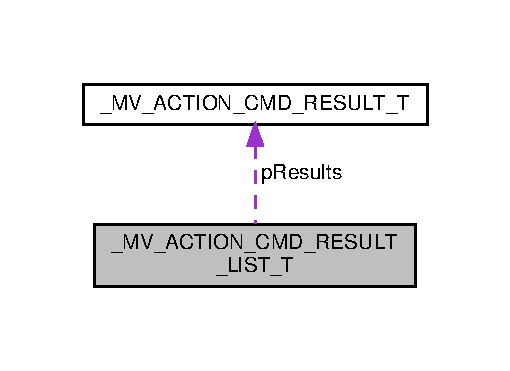
\includegraphics[width=245pt]{struct___m_v___a_c_t_i_o_n___c_m_d___r_e_s_u_l_t___l_i_s_t___t__coll__graph}
\end{center}
\end{figure}
\subsection*{Public 属性}
\begin{DoxyCompactItemize}
\item 
\mbox{\Hypertarget{struct___m_v___a_c_t_i_o_n___c_m_d___r_e_s_u_l_t___l_i_s_t___t_a57452d900f58fe3c1eb9e8b60c1f77b3}\label{struct___m_v___a_c_t_i_o_n___c_m_d___r_e_s_u_l_t___l_i_s_t___t_a57452d900f58fe3c1eb9e8b60c1f77b3}} 
unsigned int {\bfseries n\+Num\+Results}
\item 
\mbox{\Hypertarget{struct___m_v___a_c_t_i_o_n___c_m_d___r_e_s_u_l_t___l_i_s_t___t_a9b1885e995f66a512450edadb8681331}\label{struct___m_v___a_c_t_i_o_n___c_m_d___r_e_s_u_l_t___l_i_s_t___t_a9b1885e995f66a512450edadb8681331}} 
\hyperlink{struct___m_v___a_c_t_i_o_n___c_m_d___r_e_s_u_l_t___t}{M\+V\+\_\+\+A\+C\+T\+I\+O\+N\+\_\+\+C\+M\+D\+\_\+\+R\+E\+S\+U\+LT} $\ast$ {\bfseries p\+Results}
\end{DoxyCompactItemize}


该结构体的文档由以下文件生成\+:\begin{DoxyCompactItemize}
\item 
camera/hikvision/include/Camera\+Params.\+h\end{DoxyCompactItemize}

\hypertarget{struct___m_v___a_c_t_i_o_n___c_m_d___r_e_s_u_l_t___t}{}\section{\+\_\+\+M\+V\+\_\+\+A\+C\+T\+I\+O\+N\+\_\+\+C\+M\+D\+\_\+\+R\+E\+S\+U\+L\+T\+\_\+\+T结构体 参考}
\label{struct___m_v___a_c_t_i_o_n___c_m_d___r_e_s_u_l_t___t}\index{\+\_\+\+M\+V\+\_\+\+A\+C\+T\+I\+O\+N\+\_\+\+C\+M\+D\+\_\+\+R\+E\+S\+U\+L\+T\+\_\+T@{\+\_\+\+M\+V\+\_\+\+A\+C\+T\+I\+O\+N\+\_\+\+C\+M\+D\+\_\+\+R\+E\+S\+U\+L\+T\+\_\+T}}
\subsection*{Public 属性}
\begin{DoxyCompactItemize}
\item 
\mbox{\Hypertarget{struct___m_v___a_c_t_i_o_n___c_m_d___r_e_s_u_l_t___t_a923564eb4a6ab038c643894442363c3b}\label{struct___m_v___a_c_t_i_o_n___c_m_d___r_e_s_u_l_t___t_a923564eb4a6ab038c643894442363c3b}} 
unsigned char {\bfseries str\+Device\+Address} \mbox{[}12+3+1\mbox{]}
\item 
\mbox{\Hypertarget{struct___m_v___a_c_t_i_o_n___c_m_d___r_e_s_u_l_t___t_a2d617aa5f2977267f1db9195460e9e27}\label{struct___m_v___a_c_t_i_o_n___c_m_d___r_e_s_u_l_t___t_a2d617aa5f2977267f1db9195460e9e27}} 
int {\bfseries n\+Status}
\item 
\mbox{\Hypertarget{struct___m_v___a_c_t_i_o_n___c_m_d___r_e_s_u_l_t___t_a34af86a0cdbfa2f7d01de559f1358f7b}\label{struct___m_v___a_c_t_i_o_n___c_m_d___r_e_s_u_l_t___t_a34af86a0cdbfa2f7d01de559f1358f7b}} 
unsigned int {\bfseries n\+Reserved} \mbox{[}4\mbox{]}
\end{DoxyCompactItemize}


该结构体的文档由以下文件生成\+:\begin{DoxyCompactItemize}
\item 
camera/hikvision/include/Camera\+Params.\+h\end{DoxyCompactItemize}

\hypertarget{struct___m_v___a_l_l___m_a_t_c_h___i_n_f_o__}{}\section{\+\_\+\+M\+V\+\_\+\+A\+L\+L\+\_\+\+M\+A\+T\+C\+H\+\_\+\+I\+N\+F\+O\+\_\+结构体 参考}
\label{struct___m_v___a_l_l___m_a_t_c_h___i_n_f_o__}\index{\+\_\+\+M\+V\+\_\+\+A\+L\+L\+\_\+\+M\+A\+T\+C\+H\+\_\+\+I\+N\+F\+O\+\_\+@{\+\_\+\+M\+V\+\_\+\+A\+L\+L\+\_\+\+M\+A\+T\+C\+H\+\_\+\+I\+N\+F\+O\+\_\+}}
\subsection*{Public 属性}
\begin{DoxyCompactItemize}
\item 
\mbox{\Hypertarget{struct___m_v___a_l_l___m_a_t_c_h___i_n_f_o___a27039421eb5c83c9d6a0382abfb08b7e}\label{struct___m_v___a_l_l___m_a_t_c_h___i_n_f_o___a27039421eb5c83c9d6a0382abfb08b7e}} 
unsigned int {\bfseries n\+Type}
\item 
\mbox{\Hypertarget{struct___m_v___a_l_l___m_a_t_c_h___i_n_f_o___ada17fb4ac2a88aba05c4742ef6a13071}\label{struct___m_v___a_l_l___m_a_t_c_h___i_n_f_o___ada17fb4ac2a88aba05c4742ef6a13071}} 
void $\ast$ {\bfseries p\+Info}
\item 
\mbox{\Hypertarget{struct___m_v___a_l_l___m_a_t_c_h___i_n_f_o___a16de9f1db509067d0dde2c182bfe446d}\label{struct___m_v___a_l_l___m_a_t_c_h___i_n_f_o___a16de9f1db509067d0dde2c182bfe446d}} 
unsigned int {\bfseries n\+Info\+Size}
\end{DoxyCompactItemize}


该结构体的文档由以下文件生成\+:\begin{DoxyCompactItemize}
\item 
camera/hikvision/include/Camera\+Params.\+h\end{DoxyCompactItemize}

\hypertarget{struct___m_v___cam_l___d_e_v___i_n_f_o__}{}\section{\+\_\+\+M\+V\+\_\+\+Cam\+L\+\_\+\+D\+E\+V\+\_\+\+I\+N\+F\+O\+\_\+结构体 参考}
\label{struct___m_v___cam_l___d_e_v___i_n_f_o__}\index{\+\_\+\+M\+V\+\_\+\+Cam\+L\+\_\+\+D\+E\+V\+\_\+\+I\+N\+F\+O\+\_\+@{\+\_\+\+M\+V\+\_\+\+Cam\+L\+\_\+\+D\+E\+V\+\_\+\+I\+N\+F\+O\+\_\+}}
\subsection*{Public 属性}
\begin{DoxyCompactItemize}
\item 
\mbox{\Hypertarget{struct___m_v___cam_l___d_e_v___i_n_f_o___a875189c5b6a19300f9c6955221754d8f}\label{struct___m_v___cam_l___d_e_v___i_n_f_o___a875189c5b6a19300f9c6955221754d8f}} 
unsigned char {\bfseries ch\+Port\+ID} \mbox{[}I\+N\+F\+O\+\_\+\+M\+A\+X\+\_\+\+B\+U\+F\+F\+E\+R\+\_\+\+S\+I\+ZE\mbox{]}
\item 
\mbox{\Hypertarget{struct___m_v___cam_l___d_e_v___i_n_f_o___a13e36ddef6f03268754d3a15ec94353c}\label{struct___m_v___cam_l___d_e_v___i_n_f_o___a13e36ddef6f03268754d3a15ec94353c}} 
unsigned char {\bfseries ch\+Model\+Name} \mbox{[}I\+N\+F\+O\+\_\+\+M\+A\+X\+\_\+\+B\+U\+F\+F\+E\+R\+\_\+\+S\+I\+ZE\mbox{]}
\item 
\mbox{\Hypertarget{struct___m_v___cam_l___d_e_v___i_n_f_o___a0717da84d70cf3424ab872df7a3c1043}\label{struct___m_v___cam_l___d_e_v___i_n_f_o___a0717da84d70cf3424ab872df7a3c1043}} 
unsigned char {\bfseries ch\+Family\+Name} \mbox{[}I\+N\+F\+O\+\_\+\+M\+A\+X\+\_\+\+B\+U\+F\+F\+E\+R\+\_\+\+S\+I\+ZE\mbox{]}
\item 
\mbox{\Hypertarget{struct___m_v___cam_l___d_e_v___i_n_f_o___ad502c993f6f9e8fafc1caf1e16db73a9}\label{struct___m_v___cam_l___d_e_v___i_n_f_o___ad502c993f6f9e8fafc1caf1e16db73a9}} 
unsigned char {\bfseries ch\+Device\+Version} \mbox{[}I\+N\+F\+O\+\_\+\+M\+A\+X\+\_\+\+B\+U\+F\+F\+E\+R\+\_\+\+S\+I\+ZE\mbox{]}
\item 
\mbox{\Hypertarget{struct___m_v___cam_l___d_e_v___i_n_f_o___a2ddce04a73a05680b456b649532cd6f5}\label{struct___m_v___cam_l___d_e_v___i_n_f_o___a2ddce04a73a05680b456b649532cd6f5}} 
unsigned char {\bfseries ch\+Manufacturer\+Name} \mbox{[}I\+N\+F\+O\+\_\+\+M\+A\+X\+\_\+\+B\+U\+F\+F\+E\+R\+\_\+\+S\+I\+ZE\mbox{]}
\item 
\mbox{\Hypertarget{struct___m_v___cam_l___d_e_v___i_n_f_o___a0234a0a909a88172d8006f4d46cb3abe}\label{struct___m_v___cam_l___d_e_v___i_n_f_o___a0234a0a909a88172d8006f4d46cb3abe}} 
unsigned char {\bfseries ch\+Serial\+Number} \mbox{[}I\+N\+F\+O\+\_\+\+M\+A\+X\+\_\+\+B\+U\+F\+F\+E\+R\+\_\+\+S\+I\+ZE\mbox{]}
\item 
\mbox{\Hypertarget{struct___m_v___cam_l___d_e_v___i_n_f_o___a96a3dfa368b8f71482bb7b931cb0fb9e}\label{struct___m_v___cam_l___d_e_v___i_n_f_o___a96a3dfa368b8f71482bb7b931cb0fb9e}} 
unsigned int {\bfseries n\+Reserved} \mbox{[}38\mbox{]}
\end{DoxyCompactItemize}


该结构体的文档由以下文件生成\+:\begin{DoxyCompactItemize}
\item 
camera/hikvision/include/Camera\+Params.\+h\end{DoxyCompactItemize}

\hypertarget{struct___m_v___c_c___d_e_v_i_c_e___i_n_f_o__}{}\section{\+\_\+\+M\+V\+\_\+\+C\+C\+\_\+\+D\+E\+V\+I\+C\+E\+\_\+\+I\+N\+F\+O\+\_\+结构体 参考}
\label{struct___m_v___c_c___d_e_v_i_c_e___i_n_f_o__}\index{\+\_\+\+M\+V\+\_\+\+C\+C\+\_\+\+D\+E\+V\+I\+C\+E\+\_\+\+I\+N\+F\+O\+\_\+@{\+\_\+\+M\+V\+\_\+\+C\+C\+\_\+\+D\+E\+V\+I\+C\+E\+\_\+\+I\+N\+F\+O\+\_\+}}


\+\_\+\+M\+V\+\_\+\+C\+C\+\_\+\+D\+E\+V\+I\+C\+E\+\_\+\+I\+N\+F\+O\+\_\+ 的协作图\+:\nopagebreak
\begin{figure}[H]
\begin{center}
\leavevmode
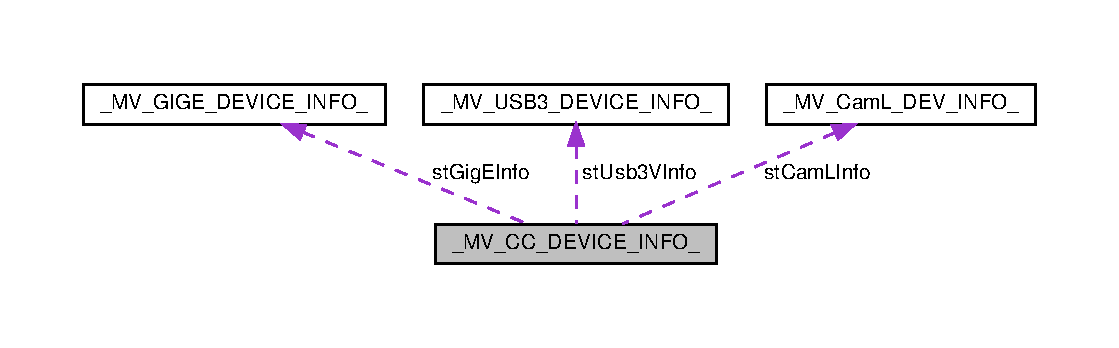
\includegraphics[width=350pt]{struct___m_v___c_c___d_e_v_i_c_e___i_n_f_o____coll__graph}
\end{center}
\end{figure}
\subsection*{Public 属性}
\begin{DoxyCompactItemize}
\item 
\mbox{\Hypertarget{struct___m_v___c_c___d_e_v_i_c_e___i_n_f_o___a2f0773023a30eb4f4c566b77325c81f6}\label{struct___m_v___c_c___d_e_v_i_c_e___i_n_f_o___a2f0773023a30eb4f4c566b77325c81f6}} 
unsigned short {\bfseries n\+Major\+Ver}
\item 
\mbox{\Hypertarget{struct___m_v___c_c___d_e_v_i_c_e___i_n_f_o___a2fc3088e0c5ece78830fa3109ff1a8cf}\label{struct___m_v___c_c___d_e_v_i_c_e___i_n_f_o___a2fc3088e0c5ece78830fa3109ff1a8cf}} 
unsigned short {\bfseries n\+Minor\+Ver}
\item 
\mbox{\Hypertarget{struct___m_v___c_c___d_e_v_i_c_e___i_n_f_o___a3d7fa64d79affd9791b80404e15fe002}\label{struct___m_v___c_c___d_e_v_i_c_e___i_n_f_o___a3d7fa64d79affd9791b80404e15fe002}} 
unsigned int {\bfseries n\+Mac\+Addr\+High}
\item 
\mbox{\Hypertarget{struct___m_v___c_c___d_e_v_i_c_e___i_n_f_o___a72d31babc7667c0f59c4c6c8b63c3d5e}\label{struct___m_v___c_c___d_e_v_i_c_e___i_n_f_o___a72d31babc7667c0f59c4c6c8b63c3d5e}} 
unsigned int {\bfseries n\+Mac\+Addr\+Low}
\item 
\mbox{\Hypertarget{struct___m_v___c_c___d_e_v_i_c_e___i_n_f_o___a3f584638615b808872a94355c3e51571}\label{struct___m_v___c_c___d_e_v_i_c_e___i_n_f_o___a3f584638615b808872a94355c3e51571}} 
unsigned int {\bfseries n\+T\+Layer\+Type}
\item 
\mbox{\Hypertarget{struct___m_v___c_c___d_e_v_i_c_e___i_n_f_o___a6ab03682fe39ec564a6b9d23a8572fd6}\label{struct___m_v___c_c___d_e_v_i_c_e___i_n_f_o___a6ab03682fe39ec564a6b9d23a8572fd6}} 
unsigned int {\bfseries n\+Reserved} \mbox{[}4\mbox{]}
\item 
\mbox{\Hypertarget{struct___m_v___c_c___d_e_v_i_c_e___i_n_f_o___ad63551e42e627dae681fcf82056cd066}\label{struct___m_v___c_c___d_e_v_i_c_e___i_n_f_o___ad63551e42e627dae681fcf82056cd066}} 
\begin{tabbing}
xx\=xx\=xx\=xx\=xx\=xx\=xx\=xx\=xx\=\kill
union \{\\
\>\hyperlink{struct___m_v___g_i_g_e___d_e_v_i_c_e___i_n_f_o__}{MV\_GIGE\_DEVICE\_INFO} {\bfseries stGigEInfo}\\
\>\hyperlink{struct___m_v___u_s_b3___d_e_v_i_c_e___i_n_f_o__}{MV\_USB3\_DEVICE\_INFO} {\bfseries stUsb3VInfo}\\
\>\hyperlink{struct___m_v___cam_l___d_e_v___i_n_f_o__}{MV\_CamL\_DEV\_INFO} {\bfseries stCamLInfo}\\
\} {\bfseries SpecialInfo}\\

\end{tabbing}\end{DoxyCompactItemize}


该结构体的文档由以下文件生成\+:\begin{DoxyCompactItemize}
\item 
camera/hikvision/include/Camera\+Params.\+h\end{DoxyCompactItemize}

\hypertarget{struct___m_v___c_c___d_e_v_i_c_e___i_n_f_o___l_i_s_t__}{}\section{\+\_\+\+M\+V\+\_\+\+C\+C\+\_\+\+D\+E\+V\+I\+C\+E\+\_\+\+I\+N\+F\+O\+\_\+\+L\+I\+S\+T\+\_\+结构体 参考}
\label{struct___m_v___c_c___d_e_v_i_c_e___i_n_f_o___l_i_s_t__}\index{\+\_\+\+M\+V\+\_\+\+C\+C\+\_\+\+D\+E\+V\+I\+C\+E\+\_\+\+I\+N\+F\+O\+\_\+\+L\+I\+S\+T\+\_\+@{\+\_\+\+M\+V\+\_\+\+C\+C\+\_\+\+D\+E\+V\+I\+C\+E\+\_\+\+I\+N\+F\+O\+\_\+\+L\+I\+S\+T\+\_\+}}


\+\_\+\+M\+V\+\_\+\+C\+C\+\_\+\+D\+E\+V\+I\+C\+E\+\_\+\+I\+N\+F\+O\+\_\+\+L\+I\+S\+T\+\_\+ 的协作图\+:\nopagebreak
\begin{figure}[H]
\begin{center}
\leavevmode
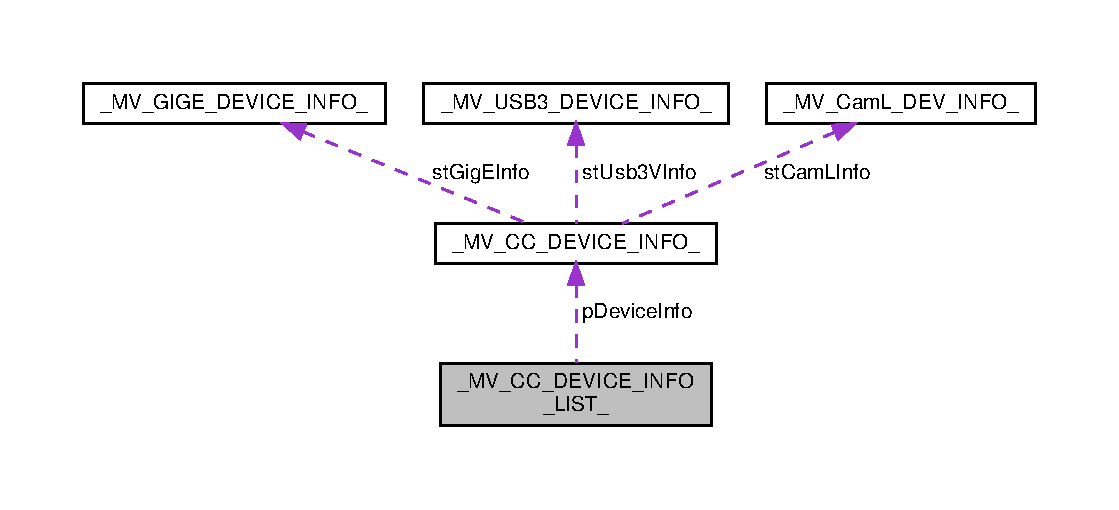
\includegraphics[width=350pt]{struct___m_v___c_c___d_e_v_i_c_e___i_n_f_o___l_i_s_t____coll__graph}
\end{center}
\end{figure}
\subsection*{Public 属性}
\begin{DoxyCompactItemize}
\item 
\mbox{\Hypertarget{struct___m_v___c_c___d_e_v_i_c_e___i_n_f_o___l_i_s_t___a04f70da14607d5d77ae965a077a7c9f8}\label{struct___m_v___c_c___d_e_v_i_c_e___i_n_f_o___l_i_s_t___a04f70da14607d5d77ae965a077a7c9f8}} 
unsigned int {\bfseries n\+Device\+Num}
\item 
\mbox{\Hypertarget{struct___m_v___c_c___d_e_v_i_c_e___i_n_f_o___l_i_s_t___a9824f768565aa8e75ddf27f80273f706}\label{struct___m_v___c_c___d_e_v_i_c_e___i_n_f_o___l_i_s_t___a9824f768565aa8e75ddf27f80273f706}} 
\hyperlink{struct___m_v___c_c___d_e_v_i_c_e___i_n_f_o__}{M\+V\+\_\+\+C\+C\+\_\+\+D\+E\+V\+I\+C\+E\+\_\+\+I\+N\+FO} $\ast$ {\bfseries p\+Device\+Info} \mbox{[}M\+V\+\_\+\+M\+A\+X\+\_\+\+D\+E\+V\+I\+C\+E\+\_\+\+N\+UM\mbox{]}
\end{DoxyCompactItemize}


该结构体的文档由以下文件生成\+:\begin{DoxyCompactItemize}
\item 
camera/hikvision/include/Camera\+Params.\+h\end{DoxyCompactItemize}

\hypertarget{struct___m_v___c_c___f_i_l_e___a_c_c_e_s_s___p_r_o_g_r_e_s_s___t}{}\section{\+\_\+\+M\+V\+\_\+\+C\+C\+\_\+\+F\+I\+L\+E\+\_\+\+A\+C\+C\+E\+S\+S\+\_\+\+P\+R\+O\+G\+R\+E\+S\+S\+\_\+\+T结构体 参考}
\label{struct___m_v___c_c___f_i_l_e___a_c_c_e_s_s___p_r_o_g_r_e_s_s___t}\index{\+\_\+\+M\+V\+\_\+\+C\+C\+\_\+\+F\+I\+L\+E\+\_\+\+A\+C\+C\+E\+S\+S\+\_\+\+P\+R\+O\+G\+R\+E\+S\+S\+\_\+T@{\+\_\+\+M\+V\+\_\+\+C\+C\+\_\+\+F\+I\+L\+E\+\_\+\+A\+C\+C\+E\+S\+S\+\_\+\+P\+R\+O\+G\+R\+E\+S\+S\+\_\+T}}
\subsection*{Public 属性}
\begin{DoxyCompactItemize}
\item 
\mbox{\Hypertarget{struct___m_v___c_c___f_i_l_e___a_c_c_e_s_s___p_r_o_g_r_e_s_s___t_afe5c39fcc87e75751353bd12286737c7}\label{struct___m_v___c_c___f_i_l_e___a_c_c_e_s_s___p_r_o_g_r_e_s_s___t_afe5c39fcc87e75751353bd12286737c7}} 
int64\+\_\+t {\bfseries n\+Completed}
\item 
\mbox{\Hypertarget{struct___m_v___c_c___f_i_l_e___a_c_c_e_s_s___p_r_o_g_r_e_s_s___t_a3e93a1876eadc94880f5a96f0339b390}\label{struct___m_v___c_c___f_i_l_e___a_c_c_e_s_s___p_r_o_g_r_e_s_s___t_a3e93a1876eadc94880f5a96f0339b390}} 
int64\+\_\+t {\bfseries n\+Total}
\item 
\mbox{\Hypertarget{struct___m_v___c_c___f_i_l_e___a_c_c_e_s_s___p_r_o_g_r_e_s_s___t_a6b7d31bc27afd2d3b75171c09cdf63d5}\label{struct___m_v___c_c___f_i_l_e___a_c_c_e_s_s___p_r_o_g_r_e_s_s___t_a6b7d31bc27afd2d3b75171c09cdf63d5}} 
unsigned int {\bfseries n\+Reserved} \mbox{[}8\mbox{]}
\end{DoxyCompactItemize}


该结构体的文档由以下文件生成\+:\begin{DoxyCompactItemize}
\item 
camera/hikvision/include/Camera\+Params.\+h\end{DoxyCompactItemize}

\hypertarget{struct___m_v___c_c___f_i_l_e___a_c_c_e_s_s___t}{}\section{\+\_\+\+M\+V\+\_\+\+C\+C\+\_\+\+F\+I\+L\+E\+\_\+\+A\+C\+C\+E\+S\+S\+\_\+\+T结构体 参考}
\label{struct___m_v___c_c___f_i_l_e___a_c_c_e_s_s___t}\index{\+\_\+\+M\+V\+\_\+\+C\+C\+\_\+\+F\+I\+L\+E\+\_\+\+A\+C\+C\+E\+S\+S\+\_\+T@{\+\_\+\+M\+V\+\_\+\+C\+C\+\_\+\+F\+I\+L\+E\+\_\+\+A\+C\+C\+E\+S\+S\+\_\+T}}
\subsection*{Public 属性}
\begin{DoxyCompactItemize}
\item 
\mbox{\Hypertarget{struct___m_v___c_c___f_i_l_e___a_c_c_e_s_s___t_a8694e31af0485f2748225fa9745695b9}\label{struct___m_v___c_c___f_i_l_e___a_c_c_e_s_s___t_a8694e31af0485f2748225fa9745695b9}} 
const char $\ast$ {\bfseries p\+User\+File\+Name}
\item 
\mbox{\Hypertarget{struct___m_v___c_c___f_i_l_e___a_c_c_e_s_s___t_af85cecdee47fb021aac43f293e490d8e}\label{struct___m_v___c_c___f_i_l_e___a_c_c_e_s_s___t_af85cecdee47fb021aac43f293e490d8e}} 
const char $\ast$ {\bfseries p\+Dev\+File\+Name}
\item 
\mbox{\Hypertarget{struct___m_v___c_c___f_i_l_e___a_c_c_e_s_s___t_aac8deb3d232d6d1056dcd9b1d1d9eeaf}\label{struct___m_v___c_c___f_i_l_e___a_c_c_e_s_s___t_aac8deb3d232d6d1056dcd9b1d1d9eeaf}} 
unsigned int {\bfseries n\+Reserved} \mbox{[}32\mbox{]}
\end{DoxyCompactItemize}


该结构体的文档由以下文件生成\+:\begin{DoxyCompactItemize}
\item 
camera/hikvision/include/Camera\+Params.\+h\end{DoxyCompactItemize}

\hypertarget{struct___m_v___c_c___i_n_p_u_t___f_r_a_m_e___i_n_f_o___t__}{}\section{\+\_\+\+M\+V\+\_\+\+C\+C\+\_\+\+I\+N\+P\+U\+T\+\_\+\+F\+R\+A\+M\+E\+\_\+\+I\+N\+F\+O\+\_\+\+T\+\_\+结构体 参考}
\label{struct___m_v___c_c___i_n_p_u_t___f_r_a_m_e___i_n_f_o___t__}\index{\+\_\+\+M\+V\+\_\+\+C\+C\+\_\+\+I\+N\+P\+U\+T\+\_\+\+F\+R\+A\+M\+E\+\_\+\+I\+N\+F\+O\+\_\+\+T\+\_\+@{\+\_\+\+M\+V\+\_\+\+C\+C\+\_\+\+I\+N\+P\+U\+T\+\_\+\+F\+R\+A\+M\+E\+\_\+\+I\+N\+F\+O\+\_\+\+T\+\_\+}}
\subsection*{Public 属性}
\begin{DoxyCompactItemize}
\item 
\mbox{\Hypertarget{struct___m_v___c_c___i_n_p_u_t___f_r_a_m_e___i_n_f_o___t___a19f127bfc24e0eec919d5c3791c1a16b}\label{struct___m_v___c_c___i_n_p_u_t___f_r_a_m_e___i_n_f_o___t___a19f127bfc24e0eec919d5c3791c1a16b}} 
unsigned char $\ast$ {\bfseries p\+Data}
\item 
\mbox{\Hypertarget{struct___m_v___c_c___i_n_p_u_t___f_r_a_m_e___i_n_f_o___t___aecb6c69b222951c61e7e342cfde3ce08}\label{struct___m_v___c_c___i_n_p_u_t___f_r_a_m_e___i_n_f_o___t___aecb6c69b222951c61e7e342cfde3ce08}} 
unsigned int {\bfseries n\+Data\+Len}
\item 
\mbox{\Hypertarget{struct___m_v___c_c___i_n_p_u_t___f_r_a_m_e___i_n_f_o___t___a15de29a5a6b0c074f64969b4bf9769b8}\label{struct___m_v___c_c___i_n_p_u_t___f_r_a_m_e___i_n_f_o___t___a15de29a5a6b0c074f64969b4bf9769b8}} 
unsigned int {\bfseries n\+Res} \mbox{[}8\mbox{]}
\end{DoxyCompactItemize}


该结构体的文档由以下文件生成\+:\begin{DoxyCompactItemize}
\item 
camera/hikvision/include/Camera\+Params.\+h\end{DoxyCompactItemize}

\hypertarget{struct___m_v___c_c___r_e_c_o_r_d___p_a_r_a_m___t__}{}\section{\+\_\+\+M\+V\+\_\+\+C\+C\+\_\+\+R\+E\+C\+O\+R\+D\+\_\+\+P\+A\+R\+A\+M\+\_\+\+T\+\_\+结构体 参考}
\label{struct___m_v___c_c___r_e_c_o_r_d___p_a_r_a_m___t__}\index{\+\_\+\+M\+V\+\_\+\+C\+C\+\_\+\+R\+E\+C\+O\+R\+D\+\_\+\+P\+A\+R\+A\+M\+\_\+\+T\+\_\+@{\+\_\+\+M\+V\+\_\+\+C\+C\+\_\+\+R\+E\+C\+O\+R\+D\+\_\+\+P\+A\+R\+A\+M\+\_\+\+T\+\_\+}}
\subsection*{Public 属性}
\begin{DoxyCompactItemize}
\item 
\mbox{\Hypertarget{struct___m_v___c_c___r_e_c_o_r_d___p_a_r_a_m___t___a32250915d5a7814a0491eb5de518e58c}\label{struct___m_v___c_c___r_e_c_o_r_d___p_a_r_a_m___t___a32250915d5a7814a0491eb5de518e58c}} 
enum Mv\+Gvsp\+Pixel\+Type {\bfseries en\+Pixel\+Type}
\item 
\mbox{\Hypertarget{struct___m_v___c_c___r_e_c_o_r_d___p_a_r_a_m___t___a3f9b88689410257f20406656a6aa52c9}\label{struct___m_v___c_c___r_e_c_o_r_d___p_a_r_a_m___t___a3f9b88689410257f20406656a6aa52c9}} 
unsigned short {\bfseries n\+Width}
\item 
\mbox{\Hypertarget{struct___m_v___c_c___r_e_c_o_r_d___p_a_r_a_m___t___a371b77ac894f16a53082bcc253d944be}\label{struct___m_v___c_c___r_e_c_o_r_d___p_a_r_a_m___t___a371b77ac894f16a53082bcc253d944be}} 
unsigned short {\bfseries n\+Height}
\item 
\mbox{\Hypertarget{struct___m_v___c_c___r_e_c_o_r_d___p_a_r_a_m___t___a33cda2cbf58ee33f59dc24c9e8130b9b}\label{struct___m_v___c_c___r_e_c_o_r_d___p_a_r_a_m___t___a33cda2cbf58ee33f59dc24c9e8130b9b}} 
float {\bfseries f\+Frame\+Rate}
\item 
\mbox{\Hypertarget{struct___m_v___c_c___r_e_c_o_r_d___p_a_r_a_m___t___a3266b44a84e2f04b3466eb31072e7141}\label{struct___m_v___c_c___r_e_c_o_r_d___p_a_r_a_m___t___a3266b44a84e2f04b3466eb31072e7141}} 
unsigned int {\bfseries n\+Bit\+Rate}
\item 
\mbox{\Hypertarget{struct___m_v___c_c___r_e_c_o_r_d___p_a_r_a_m___t___aaa923cd15757aaaf89064f6b2b9ad2db}\label{struct___m_v___c_c___r_e_c_o_r_d___p_a_r_a_m___t___aaa923cd15757aaaf89064f6b2b9ad2db}} 
M\+V\+\_\+\+R\+E\+C\+O\+R\+D\+\_\+\+F\+O\+R\+M\+A\+T\+\_\+\+T\+Y\+PE {\bfseries en\+Record\+Fmt\+Type}
\item 
\mbox{\Hypertarget{struct___m_v___c_c___r_e_c_o_r_d___p_a_r_a_m___t___ae910a2415fa44c0993a00a64e0bd5fbb}\label{struct___m_v___c_c___r_e_c_o_r_d___p_a_r_a_m___t___ae910a2415fa44c0993a00a64e0bd5fbb}} 
char $\ast$ {\bfseries str\+File\+Path}
\item 
\mbox{\Hypertarget{struct___m_v___c_c___r_e_c_o_r_d___p_a_r_a_m___t___ae557b9946d858d863ba2c47588189e57}\label{struct___m_v___c_c___r_e_c_o_r_d___p_a_r_a_m___t___ae557b9946d858d863ba2c47588189e57}} 
unsigned int {\bfseries n\+Res} \mbox{[}8\mbox{]}
\end{DoxyCompactItemize}


该结构体的文档由以下文件生成\+:\begin{DoxyCompactItemize}
\item 
camera/hikvision/include/Camera\+Params.\+h\end{DoxyCompactItemize}

\hypertarget{struct___m_v___c_h_u_n_k___d_a_t_a___c_o_n_t_e_n_t__}{}\section{\+\_\+\+M\+V\+\_\+\+C\+H\+U\+N\+K\+\_\+\+D\+A\+T\+A\+\_\+\+C\+O\+N\+T\+E\+N\+T\+\_\+结构体 参考}
\label{struct___m_v___c_h_u_n_k___d_a_t_a___c_o_n_t_e_n_t__}\index{\+\_\+\+M\+V\+\_\+\+C\+H\+U\+N\+K\+\_\+\+D\+A\+T\+A\+\_\+\+C\+O\+N\+T\+E\+N\+T\+\_\+@{\+\_\+\+M\+V\+\_\+\+C\+H\+U\+N\+K\+\_\+\+D\+A\+T\+A\+\_\+\+C\+O\+N\+T\+E\+N\+T\+\_\+}}
\subsection*{Public 属性}
\begin{DoxyCompactItemize}
\item 
\mbox{\Hypertarget{struct___m_v___c_h_u_n_k___d_a_t_a___c_o_n_t_e_n_t___ad8ca88a81060bc0d5fe76029f65c0a52}\label{struct___m_v___c_h_u_n_k___d_a_t_a___c_o_n_t_e_n_t___ad8ca88a81060bc0d5fe76029f65c0a52}} 
unsigned char $\ast$ {\bfseries p\+Chunk\+Data}
\item 
\mbox{\Hypertarget{struct___m_v___c_h_u_n_k___d_a_t_a___c_o_n_t_e_n_t___a194d104d485256a8785bc685cb019a1d}\label{struct___m_v___c_h_u_n_k___d_a_t_a___c_o_n_t_e_n_t___a194d104d485256a8785bc685cb019a1d}} 
unsigned int {\bfseries n\+Chunk\+ID}
\item 
\mbox{\Hypertarget{struct___m_v___c_h_u_n_k___d_a_t_a___c_o_n_t_e_n_t___aded61c7209d69de31123cc1369d75d26}\label{struct___m_v___c_h_u_n_k___d_a_t_a___c_o_n_t_e_n_t___aded61c7209d69de31123cc1369d75d26}} 
unsigned int {\bfseries n\+Chunk\+Len}
\item 
\mbox{\Hypertarget{struct___m_v___c_h_u_n_k___d_a_t_a___c_o_n_t_e_n_t___a96cd847befe27317fe83529e44bbde42}\label{struct___m_v___c_h_u_n_k___d_a_t_a___c_o_n_t_e_n_t___a96cd847befe27317fe83529e44bbde42}} 
unsigned int {\bfseries n\+Reserved} \mbox{[}8\mbox{]}
\end{DoxyCompactItemize}


该结构体的文档由以下文件生成\+:\begin{DoxyCompactItemize}
\item 
camera/hikvision/include/Camera\+Params.\+h\end{DoxyCompactItemize}

\hypertarget{struct___m_v___d_i_s_p_l_a_y___f_r_a_m_e___i_n_f_o__}{}\section{\+\_\+\+M\+V\+\_\+\+D\+I\+S\+P\+L\+A\+Y\+\_\+\+F\+R\+A\+M\+E\+\_\+\+I\+N\+F\+O\+\_\+结构体 参考}
\label{struct___m_v___d_i_s_p_l_a_y___f_r_a_m_e___i_n_f_o__}\index{\+\_\+\+M\+V\+\_\+\+D\+I\+S\+P\+L\+A\+Y\+\_\+\+F\+R\+A\+M\+E\+\_\+\+I\+N\+F\+O\+\_\+@{\+\_\+\+M\+V\+\_\+\+D\+I\+S\+P\+L\+A\+Y\+\_\+\+F\+R\+A\+M\+E\+\_\+\+I\+N\+F\+O\+\_\+}}
\subsection*{Public 属性}
\begin{DoxyCompactItemize}
\item 
\mbox{\Hypertarget{struct___m_v___d_i_s_p_l_a_y___f_r_a_m_e___i_n_f_o___a6223b325b3ff0f8be9d51a4e09670030}\label{struct___m_v___d_i_s_p_l_a_y___f_r_a_m_e___i_n_f_o___a6223b325b3ff0f8be9d51a4e09670030}} 
void $\ast$ {\bfseries h\+Wnd}
\item 
\mbox{\Hypertarget{struct___m_v___d_i_s_p_l_a_y___f_r_a_m_e___i_n_f_o___ad030e3defdec3be4d6a1b06563931061}\label{struct___m_v___d_i_s_p_l_a_y___f_r_a_m_e___i_n_f_o___ad030e3defdec3be4d6a1b06563931061}} 
unsigned char $\ast$ {\bfseries p\+Data}
\item 
\mbox{\Hypertarget{struct___m_v___d_i_s_p_l_a_y___f_r_a_m_e___i_n_f_o___a704362d0ebe6d3635ccedf64f6e20a09}\label{struct___m_v___d_i_s_p_l_a_y___f_r_a_m_e___i_n_f_o___a704362d0ebe6d3635ccedf64f6e20a09}} 
unsigned int {\bfseries n\+Data\+Len}
\item 
\mbox{\Hypertarget{struct___m_v___d_i_s_p_l_a_y___f_r_a_m_e___i_n_f_o___acdc9893664e857efd2e7abd1ac4c5ae5}\label{struct___m_v___d_i_s_p_l_a_y___f_r_a_m_e___i_n_f_o___acdc9893664e857efd2e7abd1ac4c5ae5}} 
unsigned short {\bfseries n\+Width}
\item 
\mbox{\Hypertarget{struct___m_v___d_i_s_p_l_a_y___f_r_a_m_e___i_n_f_o___a881be678265323edb499c1e1c7c764b5}\label{struct___m_v___d_i_s_p_l_a_y___f_r_a_m_e___i_n_f_o___a881be678265323edb499c1e1c7c764b5}} 
unsigned short {\bfseries n\+Height}
\item 
\mbox{\Hypertarget{struct___m_v___d_i_s_p_l_a_y___f_r_a_m_e___i_n_f_o___a2246b622fb4cf55732bc5045254a6b48}\label{struct___m_v___d_i_s_p_l_a_y___f_r_a_m_e___i_n_f_o___a2246b622fb4cf55732bc5045254a6b48}} 
enum Mv\+Gvsp\+Pixel\+Type {\bfseries en\+Pixel\+Type}
\item 
\mbox{\Hypertarget{struct___m_v___d_i_s_p_l_a_y___f_r_a_m_e___i_n_f_o___a95ba0c428a881eb86c7fe9fcffcde6ee}\label{struct___m_v___d_i_s_p_l_a_y___f_r_a_m_e___i_n_f_o___a95ba0c428a881eb86c7fe9fcffcde6ee}} 
unsigned int {\bfseries n\+Res} \mbox{[}4\mbox{]}
\end{DoxyCompactItemize}


该结构体的文档由以下文件生成\+:\begin{DoxyCompactItemize}
\item 
camera/hikvision/include/Camera\+Params.\+h\end{DoxyCompactItemize}

\hypertarget{struct___m_v___e_v_e_n_t___o_u_t___i_n_f_o__}{}\section{\+\_\+\+M\+V\+\_\+\+E\+V\+E\+N\+T\+\_\+\+O\+U\+T\+\_\+\+I\+N\+F\+O\+\_\+结构体 参考}
\label{struct___m_v___e_v_e_n_t___o_u_t___i_n_f_o__}\index{\+\_\+\+M\+V\+\_\+\+E\+V\+E\+N\+T\+\_\+\+O\+U\+T\+\_\+\+I\+N\+F\+O\+\_\+@{\+\_\+\+M\+V\+\_\+\+E\+V\+E\+N\+T\+\_\+\+O\+U\+T\+\_\+\+I\+N\+F\+O\+\_\+}}
\subsection*{Public 属性}
\begin{DoxyCompactItemize}
\item 
\mbox{\Hypertarget{struct___m_v___e_v_e_n_t___o_u_t___i_n_f_o___ab9331564c7173f119d43d6e642545e32}\label{struct___m_v___e_v_e_n_t___o_u_t___i_n_f_o___ab9331564c7173f119d43d6e642545e32}} 
char {\bfseries Event\+Name} \mbox{[}M\+A\+X\+\_\+\+E\+V\+E\+N\+T\+\_\+\+N\+A\+M\+E\+\_\+\+S\+I\+ZE\mbox{]}
\item 
\mbox{\Hypertarget{struct___m_v___e_v_e_n_t___o_u_t___i_n_f_o___a4b347539d0012658609bbf52be52a264}\label{struct___m_v___e_v_e_n_t___o_u_t___i_n_f_o___a4b347539d0012658609bbf52be52a264}} 
unsigned short {\bfseries n\+Event\+ID}
\item 
\mbox{\Hypertarget{struct___m_v___e_v_e_n_t___o_u_t___i_n_f_o___ac0242ad71413b3399bf87e8036b44833}\label{struct___m_v___e_v_e_n_t___o_u_t___i_n_f_o___ac0242ad71413b3399bf87e8036b44833}} 
unsigned short {\bfseries n\+Stream\+Channel}
\item 
\mbox{\Hypertarget{struct___m_v___e_v_e_n_t___o_u_t___i_n_f_o___aa6cfda658b833cd559115e9aa46d25e6}\label{struct___m_v___e_v_e_n_t___o_u_t___i_n_f_o___aa6cfda658b833cd559115e9aa46d25e6}} 
unsigned int {\bfseries n\+Block\+Id\+High}
\item 
\mbox{\Hypertarget{struct___m_v___e_v_e_n_t___o_u_t___i_n_f_o___a02cc706a80150715d80bc9d47487dc52}\label{struct___m_v___e_v_e_n_t___o_u_t___i_n_f_o___a02cc706a80150715d80bc9d47487dc52}} 
unsigned int {\bfseries n\+Block\+Id\+Low}
\item 
\mbox{\Hypertarget{struct___m_v___e_v_e_n_t___o_u_t___i_n_f_o___a072353736aa4c9b75ea2b9434f025bdb}\label{struct___m_v___e_v_e_n_t___o_u_t___i_n_f_o___a072353736aa4c9b75ea2b9434f025bdb}} 
unsigned int {\bfseries n\+Timestamp\+High}
\item 
\mbox{\Hypertarget{struct___m_v___e_v_e_n_t___o_u_t___i_n_f_o___a60774b3ce769c713ce18bcff7d64f1cc}\label{struct___m_v___e_v_e_n_t___o_u_t___i_n_f_o___a60774b3ce769c713ce18bcff7d64f1cc}} 
unsigned int {\bfseries n\+Timestamp\+Low}
\item 
\mbox{\Hypertarget{struct___m_v___e_v_e_n_t___o_u_t___i_n_f_o___a0a1f362fdac49bfe6f097f17c1977e31}\label{struct___m_v___e_v_e_n_t___o_u_t___i_n_f_o___a0a1f362fdac49bfe6f097f17c1977e31}} 
void $\ast$ {\bfseries p\+Event\+Data}
\item 
\mbox{\Hypertarget{struct___m_v___e_v_e_n_t___o_u_t___i_n_f_o___a1eb4d8cd4c4fc02f48ad9dcfea826ebd}\label{struct___m_v___e_v_e_n_t___o_u_t___i_n_f_o___a1eb4d8cd4c4fc02f48ad9dcfea826ebd}} 
unsigned int {\bfseries n\+Event\+Data\+Size}
\item 
\mbox{\Hypertarget{struct___m_v___e_v_e_n_t___o_u_t___i_n_f_o___a2f81c3c7494ee3b63e39b34c69295898}\label{struct___m_v___e_v_e_n_t___o_u_t___i_n_f_o___a2f81c3c7494ee3b63e39b34c69295898}} 
unsigned int {\bfseries n\+Reserved} \mbox{[}16\mbox{]}
\end{DoxyCompactItemize}


该结构体的文档由以下文件生成\+:\begin{DoxyCompactItemize}
\item 
camera/hikvision/include/Camera\+Params.\+h\end{DoxyCompactItemize}

\hypertarget{struct___m_v___f_r_a_m_e___o_u_t__}{}\section{\+\_\+\+M\+V\+\_\+\+F\+R\+A\+M\+E\+\_\+\+O\+U\+T\+\_\+结构体 参考}
\label{struct___m_v___f_r_a_m_e___o_u_t__}\index{\+\_\+\+M\+V\+\_\+\+F\+R\+A\+M\+E\+\_\+\+O\+U\+T\+\_\+@{\+\_\+\+M\+V\+\_\+\+F\+R\+A\+M\+E\+\_\+\+O\+U\+T\+\_\+}}


\+\_\+\+M\+V\+\_\+\+F\+R\+A\+M\+E\+\_\+\+O\+U\+T\+\_\+ 的协作图\+:\nopagebreak
\begin{figure}[H]
\begin{center}
\leavevmode
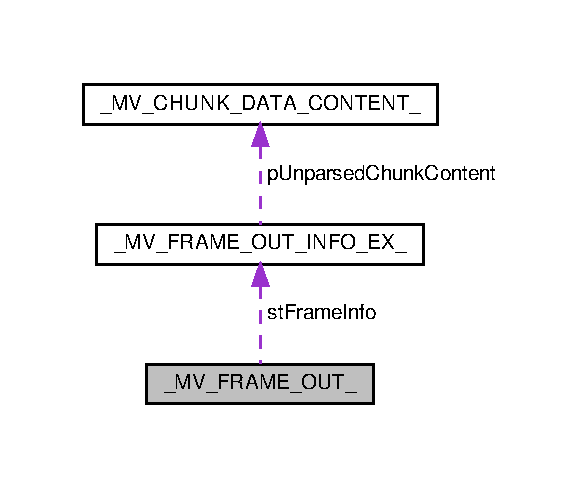
\includegraphics[width=279pt]{struct___m_v___f_r_a_m_e___o_u_t____coll__graph}
\end{center}
\end{figure}
\subsection*{Public 属性}
\begin{DoxyCompactItemize}
\item 
\mbox{\Hypertarget{struct___m_v___f_r_a_m_e___o_u_t___a5fa8908538e3adf0a0040d35edea9e0f}\label{struct___m_v___f_r_a_m_e___o_u_t___a5fa8908538e3adf0a0040d35edea9e0f}} 
unsigned char $\ast$ {\bfseries p\+Buf\+Addr}
\item 
\mbox{\Hypertarget{struct___m_v___f_r_a_m_e___o_u_t___ac733bc81d580fe0746b25f70341e450e}\label{struct___m_v___f_r_a_m_e___o_u_t___ac733bc81d580fe0746b25f70341e450e}} 
\hyperlink{struct___m_v___f_r_a_m_e___o_u_t___i_n_f_o___e_x__}{M\+V\+\_\+\+F\+R\+A\+M\+E\+\_\+\+O\+U\+T\+\_\+\+I\+N\+F\+O\+\_\+\+EX} {\bfseries st\+Frame\+Info}
\item 
\mbox{\Hypertarget{struct___m_v___f_r_a_m_e___o_u_t___ad976e77511ba4c4aa8708285507a6c18}\label{struct___m_v___f_r_a_m_e___o_u_t___ad976e77511ba4c4aa8708285507a6c18}} 
unsigned int {\bfseries n\+Res} \mbox{[}16\mbox{]}
\end{DoxyCompactItemize}


该结构体的文档由以下文件生成\+:\begin{DoxyCompactItemize}
\item 
camera/hikvision/include/Camera\+Params.\+h\end{DoxyCompactItemize}

\hypertarget{struct___m_v___f_r_a_m_e___o_u_t___i_n_f_o__}{}\section{\+\_\+\+M\+V\+\_\+\+F\+R\+A\+M\+E\+\_\+\+O\+U\+T\+\_\+\+I\+N\+F\+O\+\_\+结构体 参考}
\label{struct___m_v___f_r_a_m_e___o_u_t___i_n_f_o__}\index{\+\_\+\+M\+V\+\_\+\+F\+R\+A\+M\+E\+\_\+\+O\+U\+T\+\_\+\+I\+N\+F\+O\+\_\+@{\+\_\+\+M\+V\+\_\+\+F\+R\+A\+M\+E\+\_\+\+O\+U\+T\+\_\+\+I\+N\+F\+O\+\_\+}}
\subsection*{Public 属性}
\begin{DoxyCompactItemize}
\item 
\mbox{\Hypertarget{struct___m_v___f_r_a_m_e___o_u_t___i_n_f_o___a120f0ddafeb11cb5774bb7052fac7c73}\label{struct___m_v___f_r_a_m_e___o_u_t___i_n_f_o___a120f0ddafeb11cb5774bb7052fac7c73}} 
unsigned short {\bfseries n\+Width}
\item 
\mbox{\Hypertarget{struct___m_v___f_r_a_m_e___o_u_t___i_n_f_o___a9d1765f7047d497013578620a06598f0}\label{struct___m_v___f_r_a_m_e___o_u_t___i_n_f_o___a9d1765f7047d497013578620a06598f0}} 
unsigned short {\bfseries n\+Height}
\item 
\mbox{\Hypertarget{struct___m_v___f_r_a_m_e___o_u_t___i_n_f_o___aa737a211a43138ebc78bcd1968fd5462}\label{struct___m_v___f_r_a_m_e___o_u_t___i_n_f_o___aa737a211a43138ebc78bcd1968fd5462}} 
enum Mv\+Gvsp\+Pixel\+Type {\bfseries en\+Pixel\+Type}
\item 
\mbox{\Hypertarget{struct___m_v___f_r_a_m_e___o_u_t___i_n_f_o___a6dd94aa4313ef2ad9079fd33085bd47c}\label{struct___m_v___f_r_a_m_e___o_u_t___i_n_f_o___a6dd94aa4313ef2ad9079fd33085bd47c}} 
unsigned int {\bfseries n\+Frame\+Num}
\item 
\mbox{\Hypertarget{struct___m_v___f_r_a_m_e___o_u_t___i_n_f_o___af5ddaacd7b7f68372886155b78b26557}\label{struct___m_v___f_r_a_m_e___o_u_t___i_n_f_o___af5ddaacd7b7f68372886155b78b26557}} 
unsigned int {\bfseries n\+Dev\+Time\+Stamp\+High}
\item 
\mbox{\Hypertarget{struct___m_v___f_r_a_m_e___o_u_t___i_n_f_o___ae30f0703b40c7e9b9fca2ba3072d2f9b}\label{struct___m_v___f_r_a_m_e___o_u_t___i_n_f_o___ae30f0703b40c7e9b9fca2ba3072d2f9b}} 
unsigned int {\bfseries n\+Dev\+Time\+Stamp\+Low}
\item 
\mbox{\Hypertarget{struct___m_v___f_r_a_m_e___o_u_t___i_n_f_o___aaee8810c6f8a541764cbc7494ba0eaa7}\label{struct___m_v___f_r_a_m_e___o_u_t___i_n_f_o___aaee8810c6f8a541764cbc7494ba0eaa7}} 
unsigned int {\bfseries n\+Reserved0}
\item 
\mbox{\Hypertarget{struct___m_v___f_r_a_m_e___o_u_t___i_n_f_o___a0596cd419e5040faeeddad497a834a41}\label{struct___m_v___f_r_a_m_e___o_u_t___i_n_f_o___a0596cd419e5040faeeddad497a834a41}} 
int64\+\_\+t {\bfseries n\+Host\+Time\+Stamp}
\item 
\mbox{\Hypertarget{struct___m_v___f_r_a_m_e___o_u_t___i_n_f_o___a215b2ea05206310fd9ada3b746e241a0}\label{struct___m_v___f_r_a_m_e___o_u_t___i_n_f_o___a215b2ea05206310fd9ada3b746e241a0}} 
unsigned int {\bfseries n\+Frame\+Len}
\item 
\mbox{\Hypertarget{struct___m_v___f_r_a_m_e___o_u_t___i_n_f_o___aea15360fdf55839c648f61aa9659f7b1}\label{struct___m_v___f_r_a_m_e___o_u_t___i_n_f_o___aea15360fdf55839c648f61aa9659f7b1}} 
unsigned int {\bfseries n\+Lost\+Packet}
\item 
\mbox{\Hypertarget{struct___m_v___f_r_a_m_e___o_u_t___i_n_f_o___a0f0708abcb4079dbad4a7ed4f1e7b3ea}\label{struct___m_v___f_r_a_m_e___o_u_t___i_n_f_o___a0f0708abcb4079dbad4a7ed4f1e7b3ea}} 
unsigned int {\bfseries n\+Reserved} \mbox{[}2\mbox{]}
\end{DoxyCompactItemize}


该结构体的文档由以下文件生成\+:\begin{DoxyCompactItemize}
\item 
camera/hikvision/include/Camera\+Params.\+h\end{DoxyCompactItemize}

\hypertarget{struct___m_v___f_r_a_m_e___o_u_t___i_n_f_o___e_x__}{}\section{\+\_\+\+M\+V\+\_\+\+F\+R\+A\+M\+E\+\_\+\+O\+U\+T\+\_\+\+I\+N\+F\+O\+\_\+\+E\+X\+\_\+结构体 参考}
\label{struct___m_v___f_r_a_m_e___o_u_t___i_n_f_o___e_x__}\index{\+\_\+\+M\+V\+\_\+\+F\+R\+A\+M\+E\+\_\+\+O\+U\+T\+\_\+\+I\+N\+F\+O\+\_\+\+E\+X\+\_\+@{\+\_\+\+M\+V\+\_\+\+F\+R\+A\+M\+E\+\_\+\+O\+U\+T\+\_\+\+I\+N\+F\+O\+\_\+\+E\+X\+\_\+}}


\+\_\+\+M\+V\+\_\+\+F\+R\+A\+M\+E\+\_\+\+O\+U\+T\+\_\+\+I\+N\+F\+O\+\_\+\+E\+X\+\_\+ 的协作图\+:\nopagebreak
\begin{figure}[H]
\begin{center}
\leavevmode
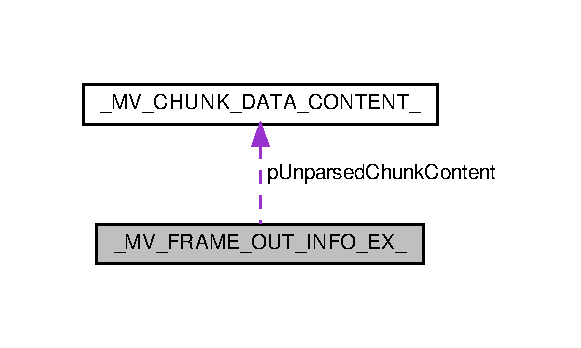
\includegraphics[width=279pt]{struct___m_v___f_r_a_m_e___o_u_t___i_n_f_o___e_x____coll__graph}
\end{center}
\end{figure}
\subsection*{Public 属性}
\begin{DoxyCompactItemize}
\item 
\mbox{\Hypertarget{struct___m_v___f_r_a_m_e___o_u_t___i_n_f_o___e_x___af6e45edcf67bd1f48453b378d2572a29}\label{struct___m_v___f_r_a_m_e___o_u_t___i_n_f_o___e_x___af6e45edcf67bd1f48453b378d2572a29}} 
unsigned short {\bfseries n\+Width}
\item 
\mbox{\Hypertarget{struct___m_v___f_r_a_m_e___o_u_t___i_n_f_o___e_x___aae9a6f9294e2f3d065526af9e4dc77a9}\label{struct___m_v___f_r_a_m_e___o_u_t___i_n_f_o___e_x___aae9a6f9294e2f3d065526af9e4dc77a9}} 
unsigned short {\bfseries n\+Height}
\item 
\mbox{\Hypertarget{struct___m_v___f_r_a_m_e___o_u_t___i_n_f_o___e_x___a07e2685d6591b3138ac792ed93bb2808}\label{struct___m_v___f_r_a_m_e___o_u_t___i_n_f_o___e_x___a07e2685d6591b3138ac792ed93bb2808}} 
enum Mv\+Gvsp\+Pixel\+Type {\bfseries en\+Pixel\+Type}
\item 
\mbox{\Hypertarget{struct___m_v___f_r_a_m_e___o_u_t___i_n_f_o___e_x___ae1a4648fba85b39a1ce550762db52597}\label{struct___m_v___f_r_a_m_e___o_u_t___i_n_f_o___e_x___ae1a4648fba85b39a1ce550762db52597}} 
unsigned int {\bfseries n\+Frame\+Num}
\item 
\mbox{\Hypertarget{struct___m_v___f_r_a_m_e___o_u_t___i_n_f_o___e_x___a04c4b878503de5919bcb8e5b12123e74}\label{struct___m_v___f_r_a_m_e___o_u_t___i_n_f_o___e_x___a04c4b878503de5919bcb8e5b12123e74}} 
unsigned int {\bfseries n\+Dev\+Time\+Stamp\+High}
\item 
\mbox{\Hypertarget{struct___m_v___f_r_a_m_e___o_u_t___i_n_f_o___e_x___a656e9c454a223b1eb1fe602843d9ae9a}\label{struct___m_v___f_r_a_m_e___o_u_t___i_n_f_o___e_x___a656e9c454a223b1eb1fe602843d9ae9a}} 
unsigned int {\bfseries n\+Dev\+Time\+Stamp\+Low}
\item 
\mbox{\Hypertarget{struct___m_v___f_r_a_m_e___o_u_t___i_n_f_o___e_x___a76fd5ce01f8bb2dd71477973d2b1e026}\label{struct___m_v___f_r_a_m_e___o_u_t___i_n_f_o___e_x___a76fd5ce01f8bb2dd71477973d2b1e026}} 
unsigned int {\bfseries n\+Reserved0}
\item 
\mbox{\Hypertarget{struct___m_v___f_r_a_m_e___o_u_t___i_n_f_o___e_x___a1e0e21e4812adcdd88d2c9ee9116408d}\label{struct___m_v___f_r_a_m_e___o_u_t___i_n_f_o___e_x___a1e0e21e4812adcdd88d2c9ee9116408d}} 
int64\+\_\+t {\bfseries n\+Host\+Time\+Stamp}
\item 
\mbox{\Hypertarget{struct___m_v___f_r_a_m_e___o_u_t___i_n_f_o___e_x___ad82adcade12d2189fe64b76f2bf96158}\label{struct___m_v___f_r_a_m_e___o_u_t___i_n_f_o___e_x___ad82adcade12d2189fe64b76f2bf96158}} 
unsigned int {\bfseries n\+Frame\+Len}
\item 
\mbox{\Hypertarget{struct___m_v___f_r_a_m_e___o_u_t___i_n_f_o___e_x___af658d7562ff72ebbb1417057a8a4ae5d}\label{struct___m_v___f_r_a_m_e___o_u_t___i_n_f_o___e_x___af658d7562ff72ebbb1417057a8a4ae5d}} 
unsigned int {\bfseries n\+Second\+Count}
\item 
\mbox{\Hypertarget{struct___m_v___f_r_a_m_e___o_u_t___i_n_f_o___e_x___acd164031fb42dd2deef47b0f7afce3db}\label{struct___m_v___f_r_a_m_e___o_u_t___i_n_f_o___e_x___acd164031fb42dd2deef47b0f7afce3db}} 
unsigned int {\bfseries n\+Cycle\+Count}
\item 
\mbox{\Hypertarget{struct___m_v___f_r_a_m_e___o_u_t___i_n_f_o___e_x___ab733ebd1097c160344038850758c04eb}\label{struct___m_v___f_r_a_m_e___o_u_t___i_n_f_o___e_x___ab733ebd1097c160344038850758c04eb}} 
unsigned int {\bfseries n\+Cycle\+Offset}
\item 
\mbox{\Hypertarget{struct___m_v___f_r_a_m_e___o_u_t___i_n_f_o___e_x___a148132f42c061ee558292f47a26cb0ce}\label{struct___m_v___f_r_a_m_e___o_u_t___i_n_f_o___e_x___a148132f42c061ee558292f47a26cb0ce}} 
float {\bfseries f\+Gain}
\item 
\mbox{\Hypertarget{struct___m_v___f_r_a_m_e___o_u_t___i_n_f_o___e_x___a88210d6161cf1b59c3c128c6c06e1299}\label{struct___m_v___f_r_a_m_e___o_u_t___i_n_f_o___e_x___a88210d6161cf1b59c3c128c6c06e1299}} 
float {\bfseries f\+Exposure\+Time}
\item 
\mbox{\Hypertarget{struct___m_v___f_r_a_m_e___o_u_t___i_n_f_o___e_x___ac9db4e845ecce80c69cd0f091da53ba3}\label{struct___m_v___f_r_a_m_e___o_u_t___i_n_f_o___e_x___ac9db4e845ecce80c69cd0f091da53ba3}} 
unsigned int {\bfseries n\+Average\+Brightness}
\item 
\mbox{\Hypertarget{struct___m_v___f_r_a_m_e___o_u_t___i_n_f_o___e_x___a6541a1623ee4743483fbecaf697dd8e5}\label{struct___m_v___f_r_a_m_e___o_u_t___i_n_f_o___e_x___a6541a1623ee4743483fbecaf697dd8e5}} 
unsigned int {\bfseries n\+Red}
\item 
\mbox{\Hypertarget{struct___m_v___f_r_a_m_e___o_u_t___i_n_f_o___e_x___a7a1a5200bb8db80d5173f7a8aae43fc5}\label{struct___m_v___f_r_a_m_e___o_u_t___i_n_f_o___e_x___a7a1a5200bb8db80d5173f7a8aae43fc5}} 
unsigned int {\bfseries n\+Green}
\item 
\mbox{\Hypertarget{struct___m_v___f_r_a_m_e___o_u_t___i_n_f_o___e_x___aaf53144c475cbf15c5fccc709d652105}\label{struct___m_v___f_r_a_m_e___o_u_t___i_n_f_o___e_x___aaf53144c475cbf15c5fccc709d652105}} 
unsigned int {\bfseries n\+Blue}
\item 
\mbox{\Hypertarget{struct___m_v___f_r_a_m_e___o_u_t___i_n_f_o___e_x___a78e5e5f44761c892e1a10521ebc2af0a}\label{struct___m_v___f_r_a_m_e___o_u_t___i_n_f_o___e_x___a78e5e5f44761c892e1a10521ebc2af0a}} 
unsigned int {\bfseries n\+Frame\+Counter}
\item 
\mbox{\Hypertarget{struct___m_v___f_r_a_m_e___o_u_t___i_n_f_o___e_x___a5c560e2b43aa342afab350d6959de97e}\label{struct___m_v___f_r_a_m_e___o_u_t___i_n_f_o___e_x___a5c560e2b43aa342afab350d6959de97e}} 
unsigned int {\bfseries n\+Trigger\+Index}
\item 
\mbox{\Hypertarget{struct___m_v___f_r_a_m_e___o_u_t___i_n_f_o___e_x___a36ee312069bc7f677f63d539bd0f96a7}\label{struct___m_v___f_r_a_m_e___o_u_t___i_n_f_o___e_x___a36ee312069bc7f677f63d539bd0f96a7}} 
unsigned int {\bfseries n\+Input}
\item 
\mbox{\Hypertarget{struct___m_v___f_r_a_m_e___o_u_t___i_n_f_o___e_x___ad8065eb562acd476dd677b1741813a34}\label{struct___m_v___f_r_a_m_e___o_u_t___i_n_f_o___e_x___ad8065eb562acd476dd677b1741813a34}} 
unsigned int {\bfseries n\+Output}
\item 
\mbox{\Hypertarget{struct___m_v___f_r_a_m_e___o_u_t___i_n_f_o___e_x___abe27c8f0e45da44714d9994abd1b8e64}\label{struct___m_v___f_r_a_m_e___o_u_t___i_n_f_o___e_x___abe27c8f0e45da44714d9994abd1b8e64}} 
unsigned short {\bfseries n\+OffsetX}
\item 
\mbox{\Hypertarget{struct___m_v___f_r_a_m_e___o_u_t___i_n_f_o___e_x___ad7fcebb85584ca60ccaf8ccb34180a3d}\label{struct___m_v___f_r_a_m_e___o_u_t___i_n_f_o___e_x___ad7fcebb85584ca60ccaf8ccb34180a3d}} 
unsigned short {\bfseries n\+OffsetY}
\item 
\mbox{\Hypertarget{struct___m_v___f_r_a_m_e___o_u_t___i_n_f_o___e_x___a54983122cf76871fe5fffa514f6699ea}\label{struct___m_v___f_r_a_m_e___o_u_t___i_n_f_o___e_x___a54983122cf76871fe5fffa514f6699ea}} 
unsigned short {\bfseries n\+Chunk\+Width}
\item 
\mbox{\Hypertarget{struct___m_v___f_r_a_m_e___o_u_t___i_n_f_o___e_x___a17d965323cf8837a1f490be3c6a8a0a8}\label{struct___m_v___f_r_a_m_e___o_u_t___i_n_f_o___e_x___a17d965323cf8837a1f490be3c6a8a0a8}} 
unsigned short {\bfseries n\+Chunk\+Height}
\item 
\mbox{\Hypertarget{struct___m_v___f_r_a_m_e___o_u_t___i_n_f_o___e_x___a98528b1898de89f63fbc5474a8a2958b}\label{struct___m_v___f_r_a_m_e___o_u_t___i_n_f_o___e_x___a98528b1898de89f63fbc5474a8a2958b}} 
unsigned int {\bfseries n\+Lost\+Packet}
\item 
\mbox{\Hypertarget{struct___m_v___f_r_a_m_e___o_u_t___i_n_f_o___e_x___a7557adbd395489a4771a5bd5656c2a59}\label{struct___m_v___f_r_a_m_e___o_u_t___i_n_f_o___e_x___a7557adbd395489a4771a5bd5656c2a59}} 
unsigned int {\bfseries n\+Unparsed\+Chunk\+Num}
\item 
\mbox{\Hypertarget{struct___m_v___f_r_a_m_e___o_u_t___i_n_f_o___e_x___a535850e43a33edfe69a713da4570bb71}\label{struct___m_v___f_r_a_m_e___o_u_t___i_n_f_o___e_x___a535850e43a33edfe69a713da4570bb71}} 
\begin{tabbing}
xx\=xx\=xx\=xx\=xx\=xx\=xx\=xx\=xx\=\kill
union \{\\
\>\hyperlink{struct___m_v___c_h_u_n_k___d_a_t_a___c_o_n_t_e_n_t__}{MV\_CHUNK\_DATA\_CONTENT} $\ast$ {\bfseries pUnparsedChunkContent}\\
\>int64\_t {\bfseries nRet}\\
\} {\bfseries UnparsedChunkList}\\

\end{tabbing}\item 
\mbox{\Hypertarget{struct___m_v___f_r_a_m_e___o_u_t___i_n_f_o___e_x___a6b17b8a0650007d00bfeed305a99d37b}\label{struct___m_v___f_r_a_m_e___o_u_t___i_n_f_o___e_x___a6b17b8a0650007d00bfeed305a99d37b}} 
unsigned int {\bfseries n\+Reserved} \mbox{[}36\mbox{]}
\end{DoxyCompactItemize}


该结构体的文档由以下文件生成\+:\begin{DoxyCompactItemize}
\item 
camera/hikvision/include/Camera\+Params.\+h\end{DoxyCompactItemize}

\hypertarget{struct___m_v___g_i_g_e___d_e_v_i_c_e___i_n_f_o__}{}\section{\+\_\+\+M\+V\+\_\+\+G\+I\+G\+E\+\_\+\+D\+E\+V\+I\+C\+E\+\_\+\+I\+N\+F\+O\+\_\+结构体 参考}
\label{struct___m_v___g_i_g_e___d_e_v_i_c_e___i_n_f_o__}\index{\+\_\+\+M\+V\+\_\+\+G\+I\+G\+E\+\_\+\+D\+E\+V\+I\+C\+E\+\_\+\+I\+N\+F\+O\+\_\+@{\+\_\+\+M\+V\+\_\+\+G\+I\+G\+E\+\_\+\+D\+E\+V\+I\+C\+E\+\_\+\+I\+N\+F\+O\+\_\+}}
\subsection*{Public 属性}
\begin{DoxyCompactItemize}
\item 
\mbox{\Hypertarget{struct___m_v___g_i_g_e___d_e_v_i_c_e___i_n_f_o___a7fea0144a1dc5bdb3b41e891ea133a9f}\label{struct___m_v___g_i_g_e___d_e_v_i_c_e___i_n_f_o___a7fea0144a1dc5bdb3b41e891ea133a9f}} 
unsigned int {\bfseries n\+Ip\+Cfg\+Option}
\item 
\mbox{\Hypertarget{struct___m_v___g_i_g_e___d_e_v_i_c_e___i_n_f_o___ac3432e221d78243fc7ece2f110ee51bf}\label{struct___m_v___g_i_g_e___d_e_v_i_c_e___i_n_f_o___ac3432e221d78243fc7ece2f110ee51bf}} 
unsigned int {\bfseries n\+Ip\+Cfg\+Current}
\item 
\mbox{\Hypertarget{struct___m_v___g_i_g_e___d_e_v_i_c_e___i_n_f_o___a1c6e5a9e358e4c24cf4bc6150ef7a909}\label{struct___m_v___g_i_g_e___d_e_v_i_c_e___i_n_f_o___a1c6e5a9e358e4c24cf4bc6150ef7a909}} 
unsigned int {\bfseries n\+Current\+Ip}
\item 
\mbox{\Hypertarget{struct___m_v___g_i_g_e___d_e_v_i_c_e___i_n_f_o___a10598d69007d2e00ed48fb6884515823}\label{struct___m_v___g_i_g_e___d_e_v_i_c_e___i_n_f_o___a10598d69007d2e00ed48fb6884515823}} 
unsigned int {\bfseries n\+Current\+Sub\+Net\+Mask}
\item 
\mbox{\Hypertarget{struct___m_v___g_i_g_e___d_e_v_i_c_e___i_n_f_o___acd2f8681f4c361d3469898cd29ed0324}\label{struct___m_v___g_i_g_e___d_e_v_i_c_e___i_n_f_o___acd2f8681f4c361d3469898cd29ed0324}} 
unsigned int {\bfseries n\+Defult\+Gate\+Way}
\item 
\mbox{\Hypertarget{struct___m_v___g_i_g_e___d_e_v_i_c_e___i_n_f_o___ae842442337bb357a7c0d80402dd09a74}\label{struct___m_v___g_i_g_e___d_e_v_i_c_e___i_n_f_o___ae842442337bb357a7c0d80402dd09a74}} 
unsigned char {\bfseries ch\+Manufacturer\+Name} \mbox{[}32\mbox{]}
\item 
\mbox{\Hypertarget{struct___m_v___g_i_g_e___d_e_v_i_c_e___i_n_f_o___ab7338402ae61dd32d57f606713c594a4}\label{struct___m_v___g_i_g_e___d_e_v_i_c_e___i_n_f_o___ab7338402ae61dd32d57f606713c594a4}} 
unsigned char {\bfseries ch\+Model\+Name} \mbox{[}32\mbox{]}
\item 
\mbox{\Hypertarget{struct___m_v___g_i_g_e___d_e_v_i_c_e___i_n_f_o___a02557eaae3ff3817896ece02cd2221e1}\label{struct___m_v___g_i_g_e___d_e_v_i_c_e___i_n_f_o___a02557eaae3ff3817896ece02cd2221e1}} 
unsigned char {\bfseries ch\+Device\+Version} \mbox{[}32\mbox{]}
\item 
\mbox{\Hypertarget{struct___m_v___g_i_g_e___d_e_v_i_c_e___i_n_f_o___a4a210f7bc01f42b0a5e92c5b95c821d1}\label{struct___m_v___g_i_g_e___d_e_v_i_c_e___i_n_f_o___a4a210f7bc01f42b0a5e92c5b95c821d1}} 
unsigned char {\bfseries ch\+Manufacturer\+Specific\+Info} \mbox{[}48\mbox{]}
\item 
\mbox{\Hypertarget{struct___m_v___g_i_g_e___d_e_v_i_c_e___i_n_f_o___afb7b3f216a8beecd7e52eac91605a03e}\label{struct___m_v___g_i_g_e___d_e_v_i_c_e___i_n_f_o___afb7b3f216a8beecd7e52eac91605a03e}} 
unsigned char {\bfseries ch\+Serial\+Number} \mbox{[}16\mbox{]}
\item 
\mbox{\Hypertarget{struct___m_v___g_i_g_e___d_e_v_i_c_e___i_n_f_o___a7d685cd94118e586748bf841215b2af8}\label{struct___m_v___g_i_g_e___d_e_v_i_c_e___i_n_f_o___a7d685cd94118e586748bf841215b2af8}} 
unsigned char {\bfseries ch\+User\+Defined\+Name} \mbox{[}16\mbox{]}
\item 
\mbox{\Hypertarget{struct___m_v___g_i_g_e___d_e_v_i_c_e___i_n_f_o___a4aa6d30162d467f795d83abaa85bce5e}\label{struct___m_v___g_i_g_e___d_e_v_i_c_e___i_n_f_o___a4aa6d30162d467f795d83abaa85bce5e}} 
unsigned int {\bfseries n\+Net\+Export}
\item 
\mbox{\Hypertarget{struct___m_v___g_i_g_e___d_e_v_i_c_e___i_n_f_o___ab6bd09927a7d373ca8cf6870defde947}\label{struct___m_v___g_i_g_e___d_e_v_i_c_e___i_n_f_o___ab6bd09927a7d373ca8cf6870defde947}} 
unsigned int {\bfseries n\+Reserved} \mbox{[}4\mbox{]}
\end{DoxyCompactItemize}


该结构体的文档由以下文件生成\+:\begin{DoxyCompactItemize}
\item 
camera/hikvision/include/Camera\+Params.\+h\end{DoxyCompactItemize}

\hypertarget{struct___m_v___i_m_a_g_e___b_a_s_i_c___i_n_f_o__}{}\section{\+\_\+\+M\+V\+\_\+\+I\+M\+A\+G\+E\+\_\+\+B\+A\+S\+I\+C\+\_\+\+I\+N\+F\+O\+\_\+结构体 参考}
\label{struct___m_v___i_m_a_g_e___b_a_s_i_c___i_n_f_o__}\index{\+\_\+\+M\+V\+\_\+\+I\+M\+A\+G\+E\+\_\+\+B\+A\+S\+I\+C\+\_\+\+I\+N\+F\+O\+\_\+@{\+\_\+\+M\+V\+\_\+\+I\+M\+A\+G\+E\+\_\+\+B\+A\+S\+I\+C\+\_\+\+I\+N\+F\+O\+\_\+}}
\subsection*{Public 属性}
\begin{DoxyCompactItemize}
\item 
\mbox{\Hypertarget{struct___m_v___i_m_a_g_e___b_a_s_i_c___i_n_f_o___ad9a54eb848020b9ed92a2a90ba6eb145}\label{struct___m_v___i_m_a_g_e___b_a_s_i_c___i_n_f_o___ad9a54eb848020b9ed92a2a90ba6eb145}} 
unsigned short {\bfseries n\+Width\+Value}
\item 
\mbox{\Hypertarget{struct___m_v___i_m_a_g_e___b_a_s_i_c___i_n_f_o___a98c4b3d1dc070c8f303ec9e7662ef73f}\label{struct___m_v___i_m_a_g_e___b_a_s_i_c___i_n_f_o___a98c4b3d1dc070c8f303ec9e7662ef73f}} 
unsigned short {\bfseries n\+Width\+Min}
\item 
\mbox{\Hypertarget{struct___m_v___i_m_a_g_e___b_a_s_i_c___i_n_f_o___a2d30ccc2be994d89a1c459a64495f30c}\label{struct___m_v___i_m_a_g_e___b_a_s_i_c___i_n_f_o___a2d30ccc2be994d89a1c459a64495f30c}} 
unsigned int {\bfseries n\+Width\+Max}
\item 
\mbox{\Hypertarget{struct___m_v___i_m_a_g_e___b_a_s_i_c___i_n_f_o___a0cb11e02b6d9e8b5f816b189ace6449e}\label{struct___m_v___i_m_a_g_e___b_a_s_i_c___i_n_f_o___a0cb11e02b6d9e8b5f816b189ace6449e}} 
unsigned int {\bfseries n\+Width\+Inc}
\item 
\mbox{\Hypertarget{struct___m_v___i_m_a_g_e___b_a_s_i_c___i_n_f_o___abab23adffb1e02282d45f7059e7d53de}\label{struct___m_v___i_m_a_g_e___b_a_s_i_c___i_n_f_o___abab23adffb1e02282d45f7059e7d53de}} 
unsigned int {\bfseries n\+Height\+Value}
\item 
\mbox{\Hypertarget{struct___m_v___i_m_a_g_e___b_a_s_i_c___i_n_f_o___a7a9b6a95b17e826818d298d337ba1599}\label{struct___m_v___i_m_a_g_e___b_a_s_i_c___i_n_f_o___a7a9b6a95b17e826818d298d337ba1599}} 
unsigned int {\bfseries n\+Height\+Min}
\item 
\mbox{\Hypertarget{struct___m_v___i_m_a_g_e___b_a_s_i_c___i_n_f_o___af58b743ad054155663180e352ece0167}\label{struct___m_v___i_m_a_g_e___b_a_s_i_c___i_n_f_o___af58b743ad054155663180e352ece0167}} 
unsigned int {\bfseries n\+Height\+Max}
\item 
\mbox{\Hypertarget{struct___m_v___i_m_a_g_e___b_a_s_i_c___i_n_f_o___aa0f86165cf2060055ff3d55b79bbe898}\label{struct___m_v___i_m_a_g_e___b_a_s_i_c___i_n_f_o___aa0f86165cf2060055ff3d55b79bbe898}} 
unsigned int {\bfseries n\+Height\+Inc}
\item 
\mbox{\Hypertarget{struct___m_v___i_m_a_g_e___b_a_s_i_c___i_n_f_o___ad403abc7eb995a3777b90ca9422d124a}\label{struct___m_v___i_m_a_g_e___b_a_s_i_c___i_n_f_o___ad403abc7eb995a3777b90ca9422d124a}} 
float {\bfseries f\+Frame\+Rate\+Value}
\item 
\mbox{\Hypertarget{struct___m_v___i_m_a_g_e___b_a_s_i_c___i_n_f_o___ae4fd9f488667869c9d215ae3826ace4c}\label{struct___m_v___i_m_a_g_e___b_a_s_i_c___i_n_f_o___ae4fd9f488667869c9d215ae3826ace4c}} 
float {\bfseries f\+Frame\+Rate\+Min}
\item 
\mbox{\Hypertarget{struct___m_v___i_m_a_g_e___b_a_s_i_c___i_n_f_o___ae36d596b4a5e15d9ed2bb5c2a5285fcc}\label{struct___m_v___i_m_a_g_e___b_a_s_i_c___i_n_f_o___ae36d596b4a5e15d9ed2bb5c2a5285fcc}} 
float {\bfseries f\+Frame\+Rate\+Max}
\item 
\mbox{\Hypertarget{struct___m_v___i_m_a_g_e___b_a_s_i_c___i_n_f_o___a5a4b584e19bc320c26c4fa7382df00e0}\label{struct___m_v___i_m_a_g_e___b_a_s_i_c___i_n_f_o___a5a4b584e19bc320c26c4fa7382df00e0}} 
unsigned int {\bfseries en\+Pixel\+Type}
\item 
\mbox{\Hypertarget{struct___m_v___i_m_a_g_e___b_a_s_i_c___i_n_f_o___a1dd23e88542e1594ce4d4042798d9992}\label{struct___m_v___i_m_a_g_e___b_a_s_i_c___i_n_f_o___a1dd23e88542e1594ce4d4042798d9992}} 
unsigned int {\bfseries n\+Supported\+Pixel\+Fmt\+Num}
\item 
\mbox{\Hypertarget{struct___m_v___i_m_a_g_e___b_a_s_i_c___i_n_f_o___aa18a69a7cef35667cb14f55c5173c315}\label{struct___m_v___i_m_a_g_e___b_a_s_i_c___i_n_f_o___aa18a69a7cef35667cb14f55c5173c315}} 
unsigned int {\bfseries en\+Pixel\+List} \mbox{[}M\+V\+\_\+\+M\+A\+X\+\_\+\+X\+M\+L\+\_\+\+S\+Y\+M\+B\+O\+L\+I\+C\+\_\+\+N\+UM\mbox{]}
\item 
\mbox{\Hypertarget{struct___m_v___i_m_a_g_e___b_a_s_i_c___i_n_f_o___a1d4ebeff557278ed23a207b74b5ec8c4}\label{struct___m_v___i_m_a_g_e___b_a_s_i_c___i_n_f_o___a1d4ebeff557278ed23a207b74b5ec8c4}} 
unsigned int {\bfseries n\+Reserved} \mbox{[}8\mbox{]}
\end{DoxyCompactItemize}


该结构体的文档由以下文件生成\+:\begin{DoxyCompactItemize}
\item 
camera/hikvision/include/Camera\+Params.\+h\end{DoxyCompactItemize}

\hypertarget{struct___m_v___m_a_t_c_h___i_n_f_o___n_e_t___d_e_t_e_c_t__}{}\section{\+\_\+\+M\+V\+\_\+\+M\+A\+T\+C\+H\+\_\+\+I\+N\+F\+O\+\_\+\+N\+E\+T\+\_\+\+D\+E\+T\+E\+C\+T\+\_\+结构体 参考}
\label{struct___m_v___m_a_t_c_h___i_n_f_o___n_e_t___d_e_t_e_c_t__}\index{\+\_\+\+M\+V\+\_\+\+M\+A\+T\+C\+H\+\_\+\+I\+N\+F\+O\+\_\+\+N\+E\+T\+\_\+\+D\+E\+T\+E\+C\+T\+\_\+@{\+\_\+\+M\+V\+\_\+\+M\+A\+T\+C\+H\+\_\+\+I\+N\+F\+O\+\_\+\+N\+E\+T\+\_\+\+D\+E\+T\+E\+C\+T\+\_\+}}
\subsection*{Public 属性}
\begin{DoxyCompactItemize}
\item 
\mbox{\Hypertarget{struct___m_v___m_a_t_c_h___i_n_f_o___n_e_t___d_e_t_e_c_t___ab028a86cc395bd06316612122d8e246a}\label{struct___m_v___m_a_t_c_h___i_n_f_o___n_e_t___d_e_t_e_c_t___ab028a86cc395bd06316612122d8e246a}} 
int64\+\_\+t {\bfseries n\+Revice\+Data\+Size}
\item 
\mbox{\Hypertarget{struct___m_v___m_a_t_c_h___i_n_f_o___n_e_t___d_e_t_e_c_t___ab21a019f6d655eb484c4b8189f695763}\label{struct___m_v___m_a_t_c_h___i_n_f_o___n_e_t___d_e_t_e_c_t___ab21a019f6d655eb484c4b8189f695763}} 
int64\+\_\+t {\bfseries n\+Lost\+Packet\+Count}
\item 
\mbox{\Hypertarget{struct___m_v___m_a_t_c_h___i_n_f_o___n_e_t___d_e_t_e_c_t___a409b30370b973ca35240b95441429554}\label{struct___m_v___m_a_t_c_h___i_n_f_o___n_e_t___d_e_t_e_c_t___a409b30370b973ca35240b95441429554}} 
unsigned int {\bfseries n\+Lost\+Frame\+Count}
\item 
\mbox{\Hypertarget{struct___m_v___m_a_t_c_h___i_n_f_o___n_e_t___d_e_t_e_c_t___a88a3dfa4e4c08cf3f1f4c256c656b3ee}\label{struct___m_v___m_a_t_c_h___i_n_f_o___n_e_t___d_e_t_e_c_t___a88a3dfa4e4c08cf3f1f4c256c656b3ee}} 
unsigned int {\bfseries n\+Net\+Recv\+Frame\+Count}
\item 
\mbox{\Hypertarget{struct___m_v___m_a_t_c_h___i_n_f_o___n_e_t___d_e_t_e_c_t___a62ef285e224910e41b8b2adf7afd4b65}\label{struct___m_v___m_a_t_c_h___i_n_f_o___n_e_t___d_e_t_e_c_t___a62ef285e224910e41b8b2adf7afd4b65}} 
int64\+\_\+t {\bfseries n\+Request\+Resend\+Packet\+Count}
\item 
\mbox{\Hypertarget{struct___m_v___m_a_t_c_h___i_n_f_o___n_e_t___d_e_t_e_c_t___a0e7f6be5e7e10ed84ee2c8443e61b795}\label{struct___m_v___m_a_t_c_h___i_n_f_o___n_e_t___d_e_t_e_c_t___a0e7f6be5e7e10ed84ee2c8443e61b795}} 
int64\+\_\+t {\bfseries n\+Resend\+Packet\+Count}
\end{DoxyCompactItemize}


该结构体的文档由以下文件生成\+:\begin{DoxyCompactItemize}
\item 
camera/hikvision/include/Camera\+Params.\+h\end{DoxyCompactItemize}

\hypertarget{struct___m_v___m_a_t_c_h___i_n_f_o___u_s_b___d_e_t_e_c_t__}{}\section{\+\_\+\+M\+V\+\_\+\+M\+A\+T\+C\+H\+\_\+\+I\+N\+F\+O\+\_\+\+U\+S\+B\+\_\+\+D\+E\+T\+E\+C\+T\+\_\+结构体 参考}
\label{struct___m_v___m_a_t_c_h___i_n_f_o___u_s_b___d_e_t_e_c_t__}\index{\+\_\+\+M\+V\+\_\+\+M\+A\+T\+C\+H\+\_\+\+I\+N\+F\+O\+\_\+\+U\+S\+B\+\_\+\+D\+E\+T\+E\+C\+T\+\_\+@{\+\_\+\+M\+V\+\_\+\+M\+A\+T\+C\+H\+\_\+\+I\+N\+F\+O\+\_\+\+U\+S\+B\+\_\+\+D\+E\+T\+E\+C\+T\+\_\+}}
\subsection*{Public 属性}
\begin{DoxyCompactItemize}
\item 
\mbox{\Hypertarget{struct___m_v___m_a_t_c_h___i_n_f_o___u_s_b___d_e_t_e_c_t___a4b7f040f54677aedcde427bf6ce486e7}\label{struct___m_v___m_a_t_c_h___i_n_f_o___u_s_b___d_e_t_e_c_t___a4b7f040f54677aedcde427bf6ce486e7}} 
int64\+\_\+t {\bfseries n\+Revice\+Data\+Size}
\item 
\mbox{\Hypertarget{struct___m_v___m_a_t_c_h___i_n_f_o___u_s_b___d_e_t_e_c_t___af017fc1e198323e56e8fafe141927d64}\label{struct___m_v___m_a_t_c_h___i_n_f_o___u_s_b___d_e_t_e_c_t___af017fc1e198323e56e8fafe141927d64}} 
unsigned int {\bfseries n\+Reviced\+Frame\+Count}
\item 
\mbox{\Hypertarget{struct___m_v___m_a_t_c_h___i_n_f_o___u_s_b___d_e_t_e_c_t___a97599aba7794c011337640dcc5f27cad}\label{struct___m_v___m_a_t_c_h___i_n_f_o___u_s_b___d_e_t_e_c_t___a97599aba7794c011337640dcc5f27cad}} 
unsigned int {\bfseries n\+Error\+Frame\+Count}
\item 
\mbox{\Hypertarget{struct___m_v___m_a_t_c_h___i_n_f_o___u_s_b___d_e_t_e_c_t___afd680884d03009c6cfcc5c192e3c3a58}\label{struct___m_v___m_a_t_c_h___i_n_f_o___u_s_b___d_e_t_e_c_t___afd680884d03009c6cfcc5c192e3c3a58}} 
unsigned int {\bfseries n\+Reserved} \mbox{[}2\mbox{]}
\end{DoxyCompactItemize}


该结构体的文档由以下文件生成\+:\begin{DoxyCompactItemize}
\item 
camera/hikvision/include/Camera\+Params.\+h\end{DoxyCompactItemize}

\hypertarget{struct___m_v___n_e_t_t_r_a_n_s___i_n_f_o__}{}\section{\+\_\+\+M\+V\+\_\+\+N\+E\+T\+T\+R\+A\+N\+S\+\_\+\+I\+N\+F\+O\+\_\+结构体 参考}
\label{struct___m_v___n_e_t_t_r_a_n_s___i_n_f_o__}\index{\+\_\+\+M\+V\+\_\+\+N\+E\+T\+T\+R\+A\+N\+S\+\_\+\+I\+N\+F\+O\+\_\+@{\+\_\+\+M\+V\+\_\+\+N\+E\+T\+T\+R\+A\+N\+S\+\_\+\+I\+N\+F\+O\+\_\+}}
\subsection*{Public 属性}
\begin{DoxyCompactItemize}
\item 
\mbox{\Hypertarget{struct___m_v___n_e_t_t_r_a_n_s___i_n_f_o___ad48ccebc2156f26407f0b4783c1d417c}\label{struct___m_v___n_e_t_t_r_a_n_s___i_n_f_o___ad48ccebc2156f26407f0b4783c1d417c}} 
int64\+\_\+t {\bfseries n\+Revice\+Data\+Size}
\item 
\mbox{\Hypertarget{struct___m_v___n_e_t_t_r_a_n_s___i_n_f_o___a7f0b15c03ddb153e6e76d073d48b006e}\label{struct___m_v___n_e_t_t_r_a_n_s___i_n_f_o___a7f0b15c03ddb153e6e76d073d48b006e}} 
int {\bfseries n\+Throw\+Frame\+Count}
\item 
\mbox{\Hypertarget{struct___m_v___n_e_t_t_r_a_n_s___i_n_f_o___a9f1c2ba3699a884a703f570945d84ad8}\label{struct___m_v___n_e_t_t_r_a_n_s___i_n_f_o___a9f1c2ba3699a884a703f570945d84ad8}} 
unsigned int {\bfseries n\+Net\+Recv\+Frame\+Count}
\item 
\mbox{\Hypertarget{struct___m_v___n_e_t_t_r_a_n_s___i_n_f_o___a6ffa3c3bb49b970cf5ff4be5a59f1760}\label{struct___m_v___n_e_t_t_r_a_n_s___i_n_f_o___a6ffa3c3bb49b970cf5ff4be5a59f1760}} 
int64\+\_\+t {\bfseries n\+Request\+Resend\+Packet\+Count}
\item 
\mbox{\Hypertarget{struct___m_v___n_e_t_t_r_a_n_s___i_n_f_o___a67bc281073809296b4a38db9630925bb}\label{struct___m_v___n_e_t_t_r_a_n_s___i_n_f_o___a67bc281073809296b4a38db9630925bb}} 
int64\+\_\+t {\bfseries n\+Resend\+Packet\+Count}
\end{DoxyCompactItemize}


该结构体的文档由以下文件生成\+:\begin{DoxyCompactItemize}
\item 
camera/hikvision/include/Camera\+Params.\+h\end{DoxyCompactItemize}

\hypertarget{struct___m_v___p_i_x_e_l___c_o_n_v_e_r_t___p_a_r_a_m___t__}{}\section{\+\_\+\+M\+V\+\_\+\+P\+I\+X\+E\+L\+\_\+\+C\+O\+N\+V\+E\+R\+T\+\_\+\+P\+A\+R\+A\+M\+\_\+\+T\+\_\+结构体 参考}
\label{struct___m_v___p_i_x_e_l___c_o_n_v_e_r_t___p_a_r_a_m___t__}\index{\+\_\+\+M\+V\+\_\+\+P\+I\+X\+E\+L\+\_\+\+C\+O\+N\+V\+E\+R\+T\+\_\+\+P\+A\+R\+A\+M\+\_\+\+T\+\_\+@{\+\_\+\+M\+V\+\_\+\+P\+I\+X\+E\+L\+\_\+\+C\+O\+N\+V\+E\+R\+T\+\_\+\+P\+A\+R\+A\+M\+\_\+\+T\+\_\+}}
\subsection*{Public 属性}
\begin{DoxyCompactItemize}
\item 
\mbox{\Hypertarget{struct___m_v___p_i_x_e_l___c_o_n_v_e_r_t___p_a_r_a_m___t___a14d7899b7d256ad5f35b79ee8760abe6}\label{struct___m_v___p_i_x_e_l___c_o_n_v_e_r_t___p_a_r_a_m___t___a14d7899b7d256ad5f35b79ee8760abe6}} 
unsigned short {\bfseries n\+Width}
\item 
\mbox{\Hypertarget{struct___m_v___p_i_x_e_l___c_o_n_v_e_r_t___p_a_r_a_m___t___aacd55116c9a8c02c569f46a1f46289d2}\label{struct___m_v___p_i_x_e_l___c_o_n_v_e_r_t___p_a_r_a_m___t___aacd55116c9a8c02c569f46a1f46289d2}} 
unsigned short {\bfseries n\+Height}
\item 
\mbox{\Hypertarget{struct___m_v___p_i_x_e_l___c_o_n_v_e_r_t___p_a_r_a_m___t___a48ce2fa8a0b41b03c452971de7b4573f}\label{struct___m_v___p_i_x_e_l___c_o_n_v_e_r_t___p_a_r_a_m___t___a48ce2fa8a0b41b03c452971de7b4573f}} 
enum Mv\+Gvsp\+Pixel\+Type {\bfseries en\+Src\+Pixel\+Type}
\item 
\mbox{\Hypertarget{struct___m_v___p_i_x_e_l___c_o_n_v_e_r_t___p_a_r_a_m___t___a3694914de55efe25aea214a09ea6a161}\label{struct___m_v___p_i_x_e_l___c_o_n_v_e_r_t___p_a_r_a_m___t___a3694914de55efe25aea214a09ea6a161}} 
unsigned char $\ast$ {\bfseries p\+Src\+Data}
\item 
\mbox{\Hypertarget{struct___m_v___p_i_x_e_l___c_o_n_v_e_r_t___p_a_r_a_m___t___a6cb3e03f7b7e37e033909aaac87a3e0f}\label{struct___m_v___p_i_x_e_l___c_o_n_v_e_r_t___p_a_r_a_m___t___a6cb3e03f7b7e37e033909aaac87a3e0f}} 
unsigned int {\bfseries n\+Src\+Data\+Len}
\item 
\mbox{\Hypertarget{struct___m_v___p_i_x_e_l___c_o_n_v_e_r_t___p_a_r_a_m___t___a8c6c961fa83b22903da8b89b1e752aba}\label{struct___m_v___p_i_x_e_l___c_o_n_v_e_r_t___p_a_r_a_m___t___a8c6c961fa83b22903da8b89b1e752aba}} 
enum Mv\+Gvsp\+Pixel\+Type {\bfseries en\+Dst\+Pixel\+Type}
\item 
\mbox{\Hypertarget{struct___m_v___p_i_x_e_l___c_o_n_v_e_r_t___p_a_r_a_m___t___ab984a56eba85206960ca5c7eb9e7e40f}\label{struct___m_v___p_i_x_e_l___c_o_n_v_e_r_t___p_a_r_a_m___t___ab984a56eba85206960ca5c7eb9e7e40f}} 
unsigned char $\ast$ {\bfseries p\+Dst\+Buffer}
\item 
\mbox{\Hypertarget{struct___m_v___p_i_x_e_l___c_o_n_v_e_r_t___p_a_r_a_m___t___aa911cd52978b3762857ca3658bbd6d3d}\label{struct___m_v___p_i_x_e_l___c_o_n_v_e_r_t___p_a_r_a_m___t___aa911cd52978b3762857ca3658bbd6d3d}} 
unsigned int {\bfseries n\+Dst\+Len}
\item 
\mbox{\Hypertarget{struct___m_v___p_i_x_e_l___c_o_n_v_e_r_t___p_a_r_a_m___t___aa51f14c349b5a251fc3f66dba64291c9}\label{struct___m_v___p_i_x_e_l___c_o_n_v_e_r_t___p_a_r_a_m___t___aa51f14c349b5a251fc3f66dba64291c9}} 
unsigned int {\bfseries n\+Dst\+Buffer\+Size}
\item 
\mbox{\Hypertarget{struct___m_v___p_i_x_e_l___c_o_n_v_e_r_t___p_a_r_a_m___t___a4a2bd2160a895ea3083c1e3fe2c728a6}\label{struct___m_v___p_i_x_e_l___c_o_n_v_e_r_t___p_a_r_a_m___t___a4a2bd2160a895ea3083c1e3fe2c728a6}} 
unsigned int {\bfseries n\+Res} \mbox{[}4\mbox{]}
\end{DoxyCompactItemize}


该结构体的文档由以下文件生成\+:\begin{DoxyCompactItemize}
\item 
camera/hikvision/include/Camera\+Params.\+h\end{DoxyCompactItemize}

\hypertarget{struct___m_v___s_a_v_e___i_m_a_g_e___p_a_r_a_m___t__}{}\section{\+\_\+\+M\+V\+\_\+\+S\+A\+V\+E\+\_\+\+I\+M\+A\+G\+E\+\_\+\+P\+A\+R\+A\+M\+\_\+\+T\+\_\+结构体 参考}
\label{struct___m_v___s_a_v_e___i_m_a_g_e___p_a_r_a_m___t__}\index{\+\_\+\+M\+V\+\_\+\+S\+A\+V\+E\+\_\+\+I\+M\+A\+G\+E\+\_\+\+P\+A\+R\+A\+M\+\_\+\+T\+\_\+@{\+\_\+\+M\+V\+\_\+\+S\+A\+V\+E\+\_\+\+I\+M\+A\+G\+E\+\_\+\+P\+A\+R\+A\+M\+\_\+\+T\+\_\+}}
\subsection*{Public 属性}
\begin{DoxyCompactItemize}
\item 
\mbox{\Hypertarget{struct___m_v___s_a_v_e___i_m_a_g_e___p_a_r_a_m___t___a9ac87bdfc7cf133fbd9cefe6803a8084}\label{struct___m_v___s_a_v_e___i_m_a_g_e___p_a_r_a_m___t___a9ac87bdfc7cf133fbd9cefe6803a8084}} 
unsigned char $\ast$ {\bfseries p\+Data}
\item 
\mbox{\Hypertarget{struct___m_v___s_a_v_e___i_m_a_g_e___p_a_r_a_m___t___aef2eea9f854f62433ebb3c5fe16fdbf5}\label{struct___m_v___s_a_v_e___i_m_a_g_e___p_a_r_a_m___t___aef2eea9f854f62433ebb3c5fe16fdbf5}} 
unsigned int {\bfseries n\+Data\+Len}
\item 
\mbox{\Hypertarget{struct___m_v___s_a_v_e___i_m_a_g_e___p_a_r_a_m___t___a4fb0063be95c22b0f3748d0d1a3726d1}\label{struct___m_v___s_a_v_e___i_m_a_g_e___p_a_r_a_m___t___a4fb0063be95c22b0f3748d0d1a3726d1}} 
enum Mv\+Gvsp\+Pixel\+Type {\bfseries en\+Pixel\+Type}
\item 
\mbox{\Hypertarget{struct___m_v___s_a_v_e___i_m_a_g_e___p_a_r_a_m___t___a9f26c566f89b2583d91982779c4b0955}\label{struct___m_v___s_a_v_e___i_m_a_g_e___p_a_r_a_m___t___a9f26c566f89b2583d91982779c4b0955}} 
unsigned short {\bfseries n\+Width}
\item 
\mbox{\Hypertarget{struct___m_v___s_a_v_e___i_m_a_g_e___p_a_r_a_m___t___a5b28e6af7c7b3d20c78a43da8e839936}\label{struct___m_v___s_a_v_e___i_m_a_g_e___p_a_r_a_m___t___a5b28e6af7c7b3d20c78a43da8e839936}} 
unsigned short {\bfseries n\+Height}
\item 
\mbox{\Hypertarget{struct___m_v___s_a_v_e___i_m_a_g_e___p_a_r_a_m___t___aeade968646b962320e0f03926ca6dbf8}\label{struct___m_v___s_a_v_e___i_m_a_g_e___p_a_r_a_m___t___aeade968646b962320e0f03926ca6dbf8}} 
unsigned char $\ast$ {\bfseries p\+Image\+Buffer}
\item 
\mbox{\Hypertarget{struct___m_v___s_a_v_e___i_m_a_g_e___p_a_r_a_m___t___af60f24498c48032e6ea3a4da5dca0a46}\label{struct___m_v___s_a_v_e___i_m_a_g_e___p_a_r_a_m___t___af60f24498c48032e6ea3a4da5dca0a46}} 
unsigned int {\bfseries n\+Image\+Len}
\item 
\mbox{\Hypertarget{struct___m_v___s_a_v_e___i_m_a_g_e___p_a_r_a_m___t___adfc1b89e2aeed248df8c0000c887f436}\label{struct___m_v___s_a_v_e___i_m_a_g_e___p_a_r_a_m___t___adfc1b89e2aeed248df8c0000c887f436}} 
unsigned int {\bfseries n\+Buffer\+Size}
\item 
\mbox{\Hypertarget{struct___m_v___s_a_v_e___i_m_a_g_e___p_a_r_a_m___t___a0899dd6c4bf80d70c00ec96ce48037b6}\label{struct___m_v___s_a_v_e___i_m_a_g_e___p_a_r_a_m___t___a0899dd6c4bf80d70c00ec96ce48037b6}} 
enum M\+V\+\_\+\+S\+A\+V\+E\+\_\+\+I\+A\+M\+G\+E\+\_\+\+T\+Y\+PE {\bfseries en\+Image\+Type}
\end{DoxyCompactItemize}


该结构体的文档由以下文件生成\+:\begin{DoxyCompactItemize}
\item 
camera/hikvision/include/Camera\+Params.\+h\end{DoxyCompactItemize}

\hypertarget{struct___m_v___s_a_v_e___i_m_a_g_e___p_a_r_a_m___t___e_x__}{}\section{\+\_\+\+M\+V\+\_\+\+S\+A\+V\+E\+\_\+\+I\+M\+A\+G\+E\+\_\+\+P\+A\+R\+A\+M\+\_\+\+T\+\_\+\+E\+X\+\_\+结构体 参考}
\label{struct___m_v___s_a_v_e___i_m_a_g_e___p_a_r_a_m___t___e_x__}\index{\+\_\+\+M\+V\+\_\+\+S\+A\+V\+E\+\_\+\+I\+M\+A\+G\+E\+\_\+\+P\+A\+R\+A\+M\+\_\+\+T\+\_\+\+E\+X\+\_\+@{\+\_\+\+M\+V\+\_\+\+S\+A\+V\+E\+\_\+\+I\+M\+A\+G\+E\+\_\+\+P\+A\+R\+A\+M\+\_\+\+T\+\_\+\+E\+X\+\_\+}}
\subsection*{Public 属性}
\begin{DoxyCompactItemize}
\item 
\mbox{\Hypertarget{struct___m_v___s_a_v_e___i_m_a_g_e___p_a_r_a_m___t___e_x___a3f0aca229cacff3fd66be1fad7ad64a5}\label{struct___m_v___s_a_v_e___i_m_a_g_e___p_a_r_a_m___t___e_x___a3f0aca229cacff3fd66be1fad7ad64a5}} 
unsigned char $\ast$ {\bfseries p\+Data}
\item 
\mbox{\Hypertarget{struct___m_v___s_a_v_e___i_m_a_g_e___p_a_r_a_m___t___e_x___ad789ae03ec83401c557b44978bf11aa4}\label{struct___m_v___s_a_v_e___i_m_a_g_e___p_a_r_a_m___t___e_x___ad789ae03ec83401c557b44978bf11aa4}} 
unsigned int {\bfseries n\+Data\+Len}
\item 
\mbox{\Hypertarget{struct___m_v___s_a_v_e___i_m_a_g_e___p_a_r_a_m___t___e_x___ae456b100270f0ae769d672d8e1baf7ec}\label{struct___m_v___s_a_v_e___i_m_a_g_e___p_a_r_a_m___t___e_x___ae456b100270f0ae769d672d8e1baf7ec}} 
enum Mv\+Gvsp\+Pixel\+Type {\bfseries en\+Pixel\+Type}
\item 
\mbox{\Hypertarget{struct___m_v___s_a_v_e___i_m_a_g_e___p_a_r_a_m___t___e_x___ad692e9889809f7c21639710f22f2dfd7}\label{struct___m_v___s_a_v_e___i_m_a_g_e___p_a_r_a_m___t___e_x___ad692e9889809f7c21639710f22f2dfd7}} 
unsigned short {\bfseries n\+Width}
\item 
\mbox{\Hypertarget{struct___m_v___s_a_v_e___i_m_a_g_e___p_a_r_a_m___t___e_x___a12818aafb13231adae39d0396dfd089f}\label{struct___m_v___s_a_v_e___i_m_a_g_e___p_a_r_a_m___t___e_x___a12818aafb13231adae39d0396dfd089f}} 
unsigned short {\bfseries n\+Height}
\item 
\mbox{\Hypertarget{struct___m_v___s_a_v_e___i_m_a_g_e___p_a_r_a_m___t___e_x___a04c6dcd3c82850c2c5e6844ba7dae155}\label{struct___m_v___s_a_v_e___i_m_a_g_e___p_a_r_a_m___t___e_x___a04c6dcd3c82850c2c5e6844ba7dae155}} 
unsigned char $\ast$ {\bfseries p\+Image\+Buffer}
\item 
\mbox{\Hypertarget{struct___m_v___s_a_v_e___i_m_a_g_e___p_a_r_a_m___t___e_x___a0205541f5183ed37ed08929200246b70}\label{struct___m_v___s_a_v_e___i_m_a_g_e___p_a_r_a_m___t___e_x___a0205541f5183ed37ed08929200246b70}} 
unsigned int {\bfseries n\+Image\+Len}
\item 
\mbox{\Hypertarget{struct___m_v___s_a_v_e___i_m_a_g_e___p_a_r_a_m___t___e_x___a0ebe9f2d85d4b5204df69b5b857420a6}\label{struct___m_v___s_a_v_e___i_m_a_g_e___p_a_r_a_m___t___e_x___a0ebe9f2d85d4b5204df69b5b857420a6}} 
unsigned int {\bfseries n\+Buffer\+Size}
\item 
\mbox{\Hypertarget{struct___m_v___s_a_v_e___i_m_a_g_e___p_a_r_a_m___t___e_x___a3828a521345bf5d02d8fc4edfde87cee}\label{struct___m_v___s_a_v_e___i_m_a_g_e___p_a_r_a_m___t___e_x___a3828a521345bf5d02d8fc4edfde87cee}} 
enum M\+V\+\_\+\+S\+A\+V\+E\+\_\+\+I\+A\+M\+G\+E\+\_\+\+T\+Y\+PE {\bfseries en\+Image\+Type}
\item 
\mbox{\Hypertarget{struct___m_v___s_a_v_e___i_m_a_g_e___p_a_r_a_m___t___e_x___a14c69f55bfdc48d975534395a95aff03}\label{struct___m_v___s_a_v_e___i_m_a_g_e___p_a_r_a_m___t___e_x___a14c69f55bfdc48d975534395a95aff03}} 
unsigned int {\bfseries n\+Jpg\+Quality}
\item 
\mbox{\Hypertarget{struct___m_v___s_a_v_e___i_m_a_g_e___p_a_r_a_m___t___e_x___a66f0092c6e217ac72d484f382233f197}\label{struct___m_v___s_a_v_e___i_m_a_g_e___p_a_r_a_m___t___e_x___a66f0092c6e217ac72d484f382233f197}} 
unsigned int {\bfseries i\+Method\+Value}
\item 
\mbox{\Hypertarget{struct___m_v___s_a_v_e___i_m_a_g_e___p_a_r_a_m___t___e_x___a23bcf831860e8aadda065bc22642400e}\label{struct___m_v___s_a_v_e___i_m_a_g_e___p_a_r_a_m___t___e_x___a23bcf831860e8aadda065bc22642400e}} 
unsigned int {\bfseries n\+Reserved} \mbox{[}3\mbox{]}
\end{DoxyCompactItemize}


该结构体的文档由以下文件生成\+:\begin{DoxyCompactItemize}
\item 
camera/hikvision/include/Camera\+Params.\+h\end{DoxyCompactItemize}

\hypertarget{struct___m_v___t_r_a_n_s_m_i_s_s_i_o_n___t_y_p_e___t}{}\section{\+\_\+\+M\+V\+\_\+\+T\+R\+A\+N\+S\+M\+I\+S\+S\+I\+O\+N\+\_\+\+T\+Y\+P\+E\+\_\+\+T结构体 参考}
\label{struct___m_v___t_r_a_n_s_m_i_s_s_i_o_n___t_y_p_e___t}\index{\+\_\+\+M\+V\+\_\+\+T\+R\+A\+N\+S\+M\+I\+S\+S\+I\+O\+N\+\_\+\+T\+Y\+P\+E\+\_\+T@{\+\_\+\+M\+V\+\_\+\+T\+R\+A\+N\+S\+M\+I\+S\+S\+I\+O\+N\+\_\+\+T\+Y\+P\+E\+\_\+T}}
\subsection*{Public 属性}
\begin{DoxyCompactItemize}
\item 
\mbox{\Hypertarget{struct___m_v___t_r_a_n_s_m_i_s_s_i_o_n___t_y_p_e___t_a8ecf73405902ca872760851569aac677}\label{struct___m_v___t_r_a_n_s_m_i_s_s_i_o_n___t_y_p_e___t_a8ecf73405902ca872760851569aac677}} 
M\+V\+\_\+\+G\+I\+G\+E\+\_\+\+T\+R\+A\+N\+S\+M\+I\+S\+S\+I\+O\+N\+\_\+\+T\+Y\+PE {\bfseries en\+Transmission\+Type}
\item 
\mbox{\Hypertarget{struct___m_v___t_r_a_n_s_m_i_s_s_i_o_n___t_y_p_e___t_aeca238b80839ca5bae88a136bf653d05}\label{struct___m_v___t_r_a_n_s_m_i_s_s_i_o_n___t_y_p_e___t_aeca238b80839ca5bae88a136bf653d05}} 
unsigned int {\bfseries n\+Dest\+Ip}
\item 
\mbox{\Hypertarget{struct___m_v___t_r_a_n_s_m_i_s_s_i_o_n___t_y_p_e___t_ae6ab52fe8268a1831f8d739033e714d1}\label{struct___m_v___t_r_a_n_s_m_i_s_s_i_o_n___t_y_p_e___t_ae6ab52fe8268a1831f8d739033e714d1}} 
unsigned short {\bfseries n\+Dest\+Port}
\item 
\mbox{\Hypertarget{struct___m_v___t_r_a_n_s_m_i_s_s_i_o_n___t_y_p_e___t_ac92f4fbc62b2ecc175ad0bb2b02dfd1c}\label{struct___m_v___t_r_a_n_s_m_i_s_s_i_o_n___t_y_p_e___t_ac92f4fbc62b2ecc175ad0bb2b02dfd1c}} 
unsigned int {\bfseries n\+Reserved} \mbox{[}32\mbox{]}
\end{DoxyCompactItemize}


该结构体的文档由以下文件生成\+:\begin{DoxyCompactItemize}
\item 
camera/hikvision/include/Camera\+Params.\+h\end{DoxyCompactItemize}

\hypertarget{struct___m_v___u_s_b3___d_e_v_i_c_e___i_n_f_o__}{}\section{\+\_\+\+M\+V\+\_\+\+U\+S\+B3\+\_\+\+D\+E\+V\+I\+C\+E\+\_\+\+I\+N\+F\+O\+\_\+结构体 参考}
\label{struct___m_v___u_s_b3___d_e_v_i_c_e___i_n_f_o__}\index{\+\_\+\+M\+V\+\_\+\+U\+S\+B3\+\_\+\+D\+E\+V\+I\+C\+E\+\_\+\+I\+N\+F\+O\+\_\+@{\+\_\+\+M\+V\+\_\+\+U\+S\+B3\+\_\+\+D\+E\+V\+I\+C\+E\+\_\+\+I\+N\+F\+O\+\_\+}}
\subsection*{Public 属性}
\begin{DoxyCompactItemize}
\item 
\mbox{\Hypertarget{struct___m_v___u_s_b3___d_e_v_i_c_e___i_n_f_o___a257befd5681410c7a7a546f913b9b071}\label{struct___m_v___u_s_b3___d_e_v_i_c_e___i_n_f_o___a257befd5681410c7a7a546f913b9b071}} 
unsigned char {\bfseries Crtl\+In\+End\+Point}
\item 
\mbox{\Hypertarget{struct___m_v___u_s_b3___d_e_v_i_c_e___i_n_f_o___a666143c07239636d1c40f77e5a2b977f}\label{struct___m_v___u_s_b3___d_e_v_i_c_e___i_n_f_o___a666143c07239636d1c40f77e5a2b977f}} 
unsigned char {\bfseries Crtl\+Out\+End\+Point}
\item 
\mbox{\Hypertarget{struct___m_v___u_s_b3___d_e_v_i_c_e___i_n_f_o___a8074d987175fd09a6dbf1f6d54e8c038}\label{struct___m_v___u_s_b3___d_e_v_i_c_e___i_n_f_o___a8074d987175fd09a6dbf1f6d54e8c038}} 
unsigned char {\bfseries Stream\+End\+Point}
\item 
\mbox{\Hypertarget{struct___m_v___u_s_b3___d_e_v_i_c_e___i_n_f_o___a5811c1c1926efb8a559a7155b99383d8}\label{struct___m_v___u_s_b3___d_e_v_i_c_e___i_n_f_o___a5811c1c1926efb8a559a7155b99383d8}} 
unsigned char {\bfseries Event\+End\+Point}
\item 
\mbox{\Hypertarget{struct___m_v___u_s_b3___d_e_v_i_c_e___i_n_f_o___a8ee688715c23deb7b6794fc736f138a2}\label{struct___m_v___u_s_b3___d_e_v_i_c_e___i_n_f_o___a8ee688715c23deb7b6794fc736f138a2}} 
unsigned short {\bfseries id\+Vendor}
\item 
\mbox{\Hypertarget{struct___m_v___u_s_b3___d_e_v_i_c_e___i_n_f_o___ae667535773400e1bc77cfd3e443b4ba3}\label{struct___m_v___u_s_b3___d_e_v_i_c_e___i_n_f_o___ae667535773400e1bc77cfd3e443b4ba3}} 
unsigned short {\bfseries id\+Product}
\item 
\mbox{\Hypertarget{struct___m_v___u_s_b3___d_e_v_i_c_e___i_n_f_o___ac197ed4dbfaee3fcfcba4209d3d674c5}\label{struct___m_v___u_s_b3___d_e_v_i_c_e___i_n_f_o___ac197ed4dbfaee3fcfcba4209d3d674c5}} 
unsigned int {\bfseries n\+Device\+Number}
\item 
\mbox{\Hypertarget{struct___m_v___u_s_b3___d_e_v_i_c_e___i_n_f_o___a5df6ff768b7a1d46d539f6a4b9ed0d61}\label{struct___m_v___u_s_b3___d_e_v_i_c_e___i_n_f_o___a5df6ff768b7a1d46d539f6a4b9ed0d61}} 
unsigned char {\bfseries ch\+Device\+G\+U\+ID} \mbox{[}I\+N\+F\+O\+\_\+\+M\+A\+X\+\_\+\+B\+U\+F\+F\+E\+R\+\_\+\+S\+I\+ZE\mbox{]}
\item 
\mbox{\Hypertarget{struct___m_v___u_s_b3___d_e_v_i_c_e___i_n_f_o___a927bcd2965442a45b35286d216251959}\label{struct___m_v___u_s_b3___d_e_v_i_c_e___i_n_f_o___a927bcd2965442a45b35286d216251959}} 
unsigned char {\bfseries ch\+Vendor\+Name} \mbox{[}I\+N\+F\+O\+\_\+\+M\+A\+X\+\_\+\+B\+U\+F\+F\+E\+R\+\_\+\+S\+I\+ZE\mbox{]}
\item 
\mbox{\Hypertarget{struct___m_v___u_s_b3___d_e_v_i_c_e___i_n_f_o___a1629fd68d248c92ab646bb58818c137b}\label{struct___m_v___u_s_b3___d_e_v_i_c_e___i_n_f_o___a1629fd68d248c92ab646bb58818c137b}} 
unsigned char {\bfseries ch\+Model\+Name} \mbox{[}I\+N\+F\+O\+\_\+\+M\+A\+X\+\_\+\+B\+U\+F\+F\+E\+R\+\_\+\+S\+I\+ZE\mbox{]}
\item 
\mbox{\Hypertarget{struct___m_v___u_s_b3___d_e_v_i_c_e___i_n_f_o___a850b1c67391906d69de9cd61b8ca33ff}\label{struct___m_v___u_s_b3___d_e_v_i_c_e___i_n_f_o___a850b1c67391906d69de9cd61b8ca33ff}} 
unsigned char {\bfseries ch\+Family\+Name} \mbox{[}I\+N\+F\+O\+\_\+\+M\+A\+X\+\_\+\+B\+U\+F\+F\+E\+R\+\_\+\+S\+I\+ZE\mbox{]}
\item 
\mbox{\Hypertarget{struct___m_v___u_s_b3___d_e_v_i_c_e___i_n_f_o___a59207b42fcef0043694cc19d0215ff6d}\label{struct___m_v___u_s_b3___d_e_v_i_c_e___i_n_f_o___a59207b42fcef0043694cc19d0215ff6d}} 
unsigned char {\bfseries ch\+Device\+Version} \mbox{[}I\+N\+F\+O\+\_\+\+M\+A\+X\+\_\+\+B\+U\+F\+F\+E\+R\+\_\+\+S\+I\+ZE\mbox{]}
\item 
\mbox{\Hypertarget{struct___m_v___u_s_b3___d_e_v_i_c_e___i_n_f_o___aafb95c61a1fb071b94c9c41ad231a546}\label{struct___m_v___u_s_b3___d_e_v_i_c_e___i_n_f_o___aafb95c61a1fb071b94c9c41ad231a546}} 
unsigned char {\bfseries ch\+Manufacturer\+Name} \mbox{[}I\+N\+F\+O\+\_\+\+M\+A\+X\+\_\+\+B\+U\+F\+F\+E\+R\+\_\+\+S\+I\+ZE\mbox{]}
\item 
\mbox{\Hypertarget{struct___m_v___u_s_b3___d_e_v_i_c_e___i_n_f_o___aa36353a498633f18647786843631cbe7}\label{struct___m_v___u_s_b3___d_e_v_i_c_e___i_n_f_o___aa36353a498633f18647786843631cbe7}} 
unsigned char {\bfseries ch\+Serial\+Number} \mbox{[}I\+N\+F\+O\+\_\+\+M\+A\+X\+\_\+\+B\+U\+F\+F\+E\+R\+\_\+\+S\+I\+ZE\mbox{]}
\item 
\mbox{\Hypertarget{struct___m_v___u_s_b3___d_e_v_i_c_e___i_n_f_o___a1feb8a6506de6f53cdff12659a5619ed}\label{struct___m_v___u_s_b3___d_e_v_i_c_e___i_n_f_o___a1feb8a6506de6f53cdff12659a5619ed}} 
unsigned char {\bfseries ch\+User\+Defined\+Name} \mbox{[}I\+N\+F\+O\+\_\+\+M\+A\+X\+\_\+\+B\+U\+F\+F\+E\+R\+\_\+\+S\+I\+ZE\mbox{]}
\item 
\mbox{\Hypertarget{struct___m_v___u_s_b3___d_e_v_i_c_e___i_n_f_o___abfe305585356ce3d8712c94b4c3e7cb6}\label{struct___m_v___u_s_b3___d_e_v_i_c_e___i_n_f_o___abfe305585356ce3d8712c94b4c3e7cb6}} 
unsigned int {\bfseries nbcd\+U\+SB}
\item 
\mbox{\Hypertarget{struct___m_v___u_s_b3___d_e_v_i_c_e___i_n_f_o___a0881861a47a9c53cef50cfa199fdc210}\label{struct___m_v___u_s_b3___d_e_v_i_c_e___i_n_f_o___a0881861a47a9c53cef50cfa199fdc210}} 
unsigned int {\bfseries n\+Reserved} \mbox{[}3\mbox{]}
\end{DoxyCompactItemize}


该结构体的文档由以下文件生成\+:\begin{DoxyCompactItemize}
\item 
camera/hikvision/include/Camera\+Params.\+h\end{DoxyCompactItemize}

\hypertarget{struct___m_v___x_m_l___c_a_m_e_r_a___f_e_a_t_u_r_e__}{}\section{\+\_\+\+M\+V\+\_\+\+X\+M\+L\+\_\+\+C\+A\+M\+E\+R\+A\+\_\+\+F\+E\+A\+T\+U\+R\+E\+\_\+结构体 参考}
\label{struct___m_v___x_m_l___c_a_m_e_r_a___f_e_a_t_u_r_e__}\index{\+\_\+\+M\+V\+\_\+\+X\+M\+L\+\_\+\+C\+A\+M\+E\+R\+A\+\_\+\+F\+E\+A\+T\+U\+R\+E\+\_\+@{\+\_\+\+M\+V\+\_\+\+X\+M\+L\+\_\+\+C\+A\+M\+E\+R\+A\+\_\+\+F\+E\+A\+T\+U\+R\+E\+\_\+}}


\+\_\+\+M\+V\+\_\+\+X\+M\+L\+\_\+\+C\+A\+M\+E\+R\+A\+\_\+\+F\+E\+A\+T\+U\+R\+E\+\_\+ 的协作图\+:\nopagebreak
\begin{figure}[H]
\begin{center}
\leavevmode
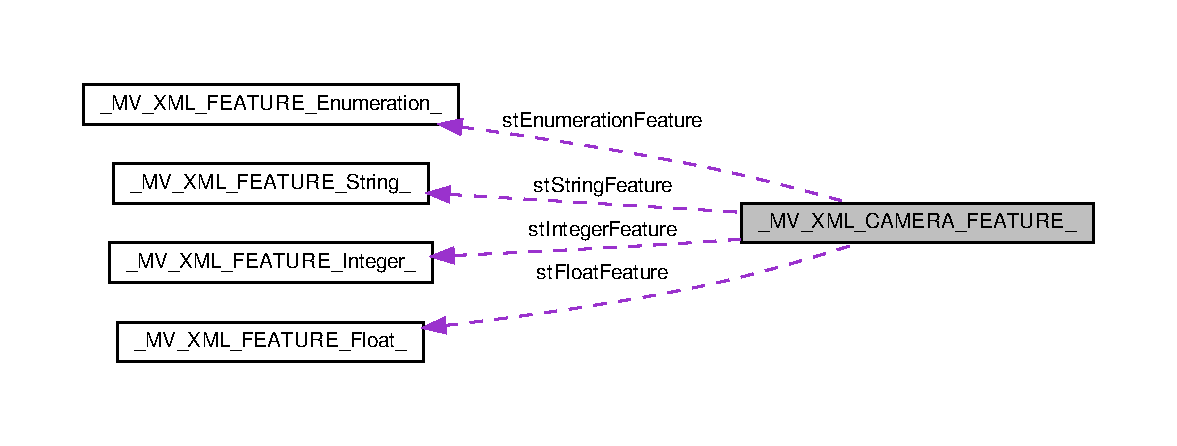
\includegraphics[width=350pt]{struct___m_v___x_m_l___c_a_m_e_r_a___f_e_a_t_u_r_e____coll__graph}
\end{center}
\end{figure}
\subsection*{Public 属性}
\begin{DoxyCompactItemize}
\item 
\mbox{\Hypertarget{struct___m_v___x_m_l___c_a_m_e_r_a___f_e_a_t_u_r_e___a5740e69af6a0b78dbf4fea7c402fa322}\label{struct___m_v___x_m_l___c_a_m_e_r_a___f_e_a_t_u_r_e___a5740e69af6a0b78dbf4fea7c402fa322}} 
enum M\+V\+\_\+\+X\+M\+L\+\_\+\+Interface\+Type {\bfseries en\+Type}
\item 
\mbox{\Hypertarget{struct___m_v___x_m_l___c_a_m_e_r_a___f_e_a_t_u_r_e___a0b1dd626f39f00083003297c61717b5f}\label{struct___m_v___x_m_l___c_a_m_e_r_a___f_e_a_t_u_r_e___a0b1dd626f39f00083003297c61717b5f}} 
\begin{tabbing}
xx\=xx\=xx\=xx\=xx\=xx\=xx\=xx\=xx\=\kill
union \{\\
\>\hyperlink{struct___m_v___x_m_l___f_e_a_t_u_r_e___integer__}{MV\_XML\_FEATURE\_Integer} {\bfseries stIntegerFeature}\\
\>\hyperlink{struct___m_v___x_m_l___f_e_a_t_u_r_e___float__}{MV\_XML\_FEATURE\_Float} {\bfseries stFloatFeature}\\
\>\hyperlink{struct___m_v___x_m_l___f_e_a_t_u_r_e___enumeration__}{MV\_XML\_FEATURE\_Enumeration} {\bfseries stEnumerationFeature}\\
\>\hyperlink{struct___m_v___x_m_l___f_e_a_t_u_r_e___string__}{MV\_XML\_FEATURE\_String} {\bfseries stStringFeature}\\
\} {\bfseries SpecialFeature}\\

\end{tabbing}\end{DoxyCompactItemize}


该结构体的文档由以下文件生成\+:\begin{DoxyCompactItemize}
\item 
camera/hikvision/include/Camera\+Params.\+h\end{DoxyCompactItemize}

\hypertarget{struct___m_v___x_m_l___f_e_a_t_u_r_e___base__}{}\section{\+\_\+\+M\+V\+\_\+\+X\+M\+L\+\_\+\+F\+E\+A\+T\+U\+R\+E\+\_\+\+Base\+\_\+结构体 参考}
\label{struct___m_v___x_m_l___f_e_a_t_u_r_e___base__}\index{\+\_\+\+M\+V\+\_\+\+X\+M\+L\+\_\+\+F\+E\+A\+T\+U\+R\+E\+\_\+\+Base\+\_\+@{\+\_\+\+M\+V\+\_\+\+X\+M\+L\+\_\+\+F\+E\+A\+T\+U\+R\+E\+\_\+\+Base\+\_\+}}
\subsection*{Public 属性}
\begin{DoxyCompactItemize}
\item 
\mbox{\Hypertarget{struct___m_v___x_m_l___f_e_a_t_u_r_e___base___aa4d95339bcb61676a0bcb1946980928a}\label{struct___m_v___x_m_l___f_e_a_t_u_r_e___base___aa4d95339bcb61676a0bcb1946980928a}} 
enum M\+V\+\_\+\+X\+M\+L\+\_\+\+Access\+Mode {\bfseries en\+Access\+Mode}
\end{DoxyCompactItemize}


该结构体的文档由以下文件生成\+:\begin{DoxyCompactItemize}
\item 
camera/hikvision/include/Camera\+Params.\+h\end{DoxyCompactItemize}

\hypertarget{struct___m_v___x_m_l___f_e_a_t_u_r_e___boolean__}{}\section{\+\_\+\+M\+V\+\_\+\+X\+M\+L\+\_\+\+F\+E\+A\+T\+U\+R\+E\+\_\+\+Boolean\+\_\+结构体 参考}
\label{struct___m_v___x_m_l___f_e_a_t_u_r_e___boolean__}\index{\+\_\+\+M\+V\+\_\+\+X\+M\+L\+\_\+\+F\+E\+A\+T\+U\+R\+E\+\_\+\+Boolean\+\_\+@{\+\_\+\+M\+V\+\_\+\+X\+M\+L\+\_\+\+F\+E\+A\+T\+U\+R\+E\+\_\+\+Boolean\+\_\+}}
\subsection*{Public 属性}
\begin{DoxyCompactItemize}
\item 
\mbox{\Hypertarget{struct___m_v___x_m_l___f_e_a_t_u_r_e___boolean___a3e6c04dc5ff22317553bcaecbcf614e6}\label{struct___m_v___x_m_l___f_e_a_t_u_r_e___boolean___a3e6c04dc5ff22317553bcaecbcf614e6}} 
char {\bfseries str\+Name} \mbox{[}M\+V\+\_\+\+M\+A\+X\+\_\+\+X\+M\+L\+\_\+\+N\+O\+D\+E\+\_\+\+S\+T\+R\+L\+E\+N\+\_\+C\mbox{]}
\item 
\mbox{\Hypertarget{struct___m_v___x_m_l___f_e_a_t_u_r_e___boolean___aefc69df31cd511024d4bc6d2219df82a}\label{struct___m_v___x_m_l___f_e_a_t_u_r_e___boolean___aefc69df31cd511024d4bc6d2219df82a}} 
char {\bfseries str\+Display\+Name} \mbox{[}M\+V\+\_\+\+M\+A\+X\+\_\+\+X\+M\+L\+\_\+\+N\+O\+D\+E\+\_\+\+S\+T\+R\+L\+E\+N\+\_\+C\mbox{]}
\item 
\mbox{\Hypertarget{struct___m_v___x_m_l___f_e_a_t_u_r_e___boolean___a93abe6f63d749950b8f353e5b9cc1f76}\label{struct___m_v___x_m_l___f_e_a_t_u_r_e___boolean___a93abe6f63d749950b8f353e5b9cc1f76}} 
char {\bfseries str\+Description} \mbox{[}M\+V\+\_\+\+M\+A\+X\+\_\+\+X\+M\+L\+\_\+\+D\+I\+S\+C\+\_\+\+S\+T\+R\+L\+E\+N\+\_\+C\mbox{]}
\item 
\mbox{\Hypertarget{struct___m_v___x_m_l___f_e_a_t_u_r_e___boolean___aa864c8fa3a118fc4ee7abdd633bc8564}\label{struct___m_v___x_m_l___f_e_a_t_u_r_e___boolean___aa864c8fa3a118fc4ee7abdd633bc8564}} 
char {\bfseries str\+Tool\+Tip} \mbox{[}M\+V\+\_\+\+M\+A\+X\+\_\+\+X\+M\+L\+\_\+\+D\+I\+S\+C\+\_\+\+S\+T\+R\+L\+E\+N\+\_\+C\mbox{]}
\item 
\mbox{\Hypertarget{struct___m_v___x_m_l___f_e_a_t_u_r_e___boolean___acb19adb676ee675729c430e8965d07bc}\label{struct___m_v___x_m_l___f_e_a_t_u_r_e___boolean___acb19adb676ee675729c430e8965d07bc}} 
enum M\+V\+\_\+\+X\+M\+L\+\_\+\+Visibility {\bfseries en\+Visivility}
\item 
\mbox{\Hypertarget{struct___m_v___x_m_l___f_e_a_t_u_r_e___boolean___a36bdc249a45955cf50a7280c2daec25a}\label{struct___m_v___x_m_l___f_e_a_t_u_r_e___boolean___a36bdc249a45955cf50a7280c2daec25a}} 
enum M\+V\+\_\+\+X\+M\+L\+\_\+\+Access\+Mode {\bfseries en\+Access\+Mode}
\item 
\mbox{\Hypertarget{struct___m_v___x_m_l___f_e_a_t_u_r_e___boolean___a269c774f1692151eedcc5f292ee289e2}\label{struct___m_v___x_m_l___f_e_a_t_u_r_e___boolean___a269c774f1692151eedcc5f292ee289e2}} 
int {\bfseries b\+Is\+Locked}
\item 
\mbox{\Hypertarget{struct___m_v___x_m_l___f_e_a_t_u_r_e___boolean___acc72256039cd7627a5245d0b3e3225ec}\label{struct___m_v___x_m_l___f_e_a_t_u_r_e___boolean___acc72256039cd7627a5245d0b3e3225ec}} 
bool {\bfseries b\+Value}
\item 
\mbox{\Hypertarget{struct___m_v___x_m_l___f_e_a_t_u_r_e___boolean___a1bac78d8c0ffc9d236952f3089ae1353}\label{struct___m_v___x_m_l___f_e_a_t_u_r_e___boolean___a1bac78d8c0ffc9d236952f3089ae1353}} 
unsigned int {\bfseries n\+Reserved} \mbox{[}4\mbox{]}
\end{DoxyCompactItemize}


该结构体的文档由以下文件生成\+:\begin{DoxyCompactItemize}
\item 
camera/hikvision/include/Camera\+Params.\+h\end{DoxyCompactItemize}

\hypertarget{struct___m_v___x_m_l___f_e_a_t_u_r_e___category__}{}\section{\+\_\+\+M\+V\+\_\+\+X\+M\+L\+\_\+\+F\+E\+A\+T\+U\+R\+E\+\_\+\+Category\+\_\+结构体 参考}
\label{struct___m_v___x_m_l___f_e_a_t_u_r_e___category__}\index{\+\_\+\+M\+V\+\_\+\+X\+M\+L\+\_\+\+F\+E\+A\+T\+U\+R\+E\+\_\+\+Category\+\_\+@{\+\_\+\+M\+V\+\_\+\+X\+M\+L\+\_\+\+F\+E\+A\+T\+U\+R\+E\+\_\+\+Category\+\_\+}}
\subsection*{Public 属性}
\begin{DoxyCompactItemize}
\item 
\mbox{\Hypertarget{struct___m_v___x_m_l___f_e_a_t_u_r_e___category___a3c1cd639385eae2dd0e35eee534cf8ab}\label{struct___m_v___x_m_l___f_e_a_t_u_r_e___category___a3c1cd639385eae2dd0e35eee534cf8ab}} 
char {\bfseries str\+Description} \mbox{[}M\+V\+\_\+\+M\+A\+X\+\_\+\+X\+M\+L\+\_\+\+D\+I\+S\+C\+\_\+\+S\+T\+R\+L\+E\+N\+\_\+C\mbox{]}
\item 
\mbox{\Hypertarget{struct___m_v___x_m_l___f_e_a_t_u_r_e___category___a82d21457a8be9268f3bb5db6112d4a66}\label{struct___m_v___x_m_l___f_e_a_t_u_r_e___category___a82d21457a8be9268f3bb5db6112d4a66}} 
char {\bfseries str\+Display\+Name} \mbox{[}M\+V\+\_\+\+M\+A\+X\+\_\+\+X\+M\+L\+\_\+\+N\+O\+D\+E\+\_\+\+S\+T\+R\+L\+E\+N\+\_\+C\mbox{]}
\item 
\mbox{\Hypertarget{struct___m_v___x_m_l___f_e_a_t_u_r_e___category___a7e561f80d50cbf102812b1a7f1eccf72}\label{struct___m_v___x_m_l___f_e_a_t_u_r_e___category___a7e561f80d50cbf102812b1a7f1eccf72}} 
char {\bfseries str\+Name} \mbox{[}M\+V\+\_\+\+M\+A\+X\+\_\+\+X\+M\+L\+\_\+\+N\+O\+D\+E\+\_\+\+S\+T\+R\+L\+E\+N\+\_\+C\mbox{]}
\item 
\mbox{\Hypertarget{struct___m_v___x_m_l___f_e_a_t_u_r_e___category___af1f46053a352c2e0ea78bde8876eb632}\label{struct___m_v___x_m_l___f_e_a_t_u_r_e___category___af1f46053a352c2e0ea78bde8876eb632}} 
char {\bfseries str\+Tool\+Tip} \mbox{[}M\+V\+\_\+\+M\+A\+X\+\_\+\+X\+M\+L\+\_\+\+D\+I\+S\+C\+\_\+\+S\+T\+R\+L\+E\+N\+\_\+C\mbox{]}
\item 
\mbox{\Hypertarget{struct___m_v___x_m_l___f_e_a_t_u_r_e___category___a6311d0a3105db376ad242dce7c8e8bbf}\label{struct___m_v___x_m_l___f_e_a_t_u_r_e___category___a6311d0a3105db376ad242dce7c8e8bbf}} 
enum M\+V\+\_\+\+X\+M\+L\+\_\+\+Visibility {\bfseries en\+Visivility}
\item 
\mbox{\Hypertarget{struct___m_v___x_m_l___f_e_a_t_u_r_e___category___abb1c55f243cb6895381e088dbebe2bf2}\label{struct___m_v___x_m_l___f_e_a_t_u_r_e___category___abb1c55f243cb6895381e088dbebe2bf2}} 
unsigned int {\bfseries n\+Reserved} \mbox{[}4\mbox{]}
\end{DoxyCompactItemize}


该结构体的文档由以下文件生成\+:\begin{DoxyCompactItemize}
\item 
camera/hikvision/include/Camera\+Params.\+h\end{DoxyCompactItemize}

\hypertarget{struct___m_v___x_m_l___f_e_a_t_u_r_e___command__}{}\section{\+\_\+\+M\+V\+\_\+\+X\+M\+L\+\_\+\+F\+E\+A\+T\+U\+R\+E\+\_\+\+Command\+\_\+结构体 参考}
\label{struct___m_v___x_m_l___f_e_a_t_u_r_e___command__}\index{\+\_\+\+M\+V\+\_\+\+X\+M\+L\+\_\+\+F\+E\+A\+T\+U\+R\+E\+\_\+\+Command\+\_\+@{\+\_\+\+M\+V\+\_\+\+X\+M\+L\+\_\+\+F\+E\+A\+T\+U\+R\+E\+\_\+\+Command\+\_\+}}
\subsection*{Public 属性}
\begin{DoxyCompactItemize}
\item 
\mbox{\Hypertarget{struct___m_v___x_m_l___f_e_a_t_u_r_e___command___adfaad6104e084d1d698d9dd7d6ba0b01}\label{struct___m_v___x_m_l___f_e_a_t_u_r_e___command___adfaad6104e084d1d698d9dd7d6ba0b01}} 
char {\bfseries str\+Name} \mbox{[}M\+V\+\_\+\+M\+A\+X\+\_\+\+X\+M\+L\+\_\+\+N\+O\+D\+E\+\_\+\+S\+T\+R\+L\+E\+N\+\_\+C\mbox{]}
\item 
\mbox{\Hypertarget{struct___m_v___x_m_l___f_e_a_t_u_r_e___command___a5ca9036eea9be00c2183cc222bdbd3cc}\label{struct___m_v___x_m_l___f_e_a_t_u_r_e___command___a5ca9036eea9be00c2183cc222bdbd3cc}} 
char {\bfseries str\+Display\+Name} \mbox{[}M\+V\+\_\+\+M\+A\+X\+\_\+\+X\+M\+L\+\_\+\+N\+O\+D\+E\+\_\+\+S\+T\+R\+L\+E\+N\+\_\+C\mbox{]}
\item 
\mbox{\Hypertarget{struct___m_v___x_m_l___f_e_a_t_u_r_e___command___a86766c6816b8c0c4abe0c9886a7bdaa3}\label{struct___m_v___x_m_l___f_e_a_t_u_r_e___command___a86766c6816b8c0c4abe0c9886a7bdaa3}} 
char {\bfseries str\+Description} \mbox{[}M\+V\+\_\+\+M\+A\+X\+\_\+\+X\+M\+L\+\_\+\+D\+I\+S\+C\+\_\+\+S\+T\+R\+L\+E\+N\+\_\+C\mbox{]}
\item 
\mbox{\Hypertarget{struct___m_v___x_m_l___f_e_a_t_u_r_e___command___ae484c9f0bed4d7609e05fd1175755588}\label{struct___m_v___x_m_l___f_e_a_t_u_r_e___command___ae484c9f0bed4d7609e05fd1175755588}} 
char {\bfseries str\+Tool\+Tip} \mbox{[}M\+V\+\_\+\+M\+A\+X\+\_\+\+X\+M\+L\+\_\+\+D\+I\+S\+C\+\_\+\+S\+T\+R\+L\+E\+N\+\_\+C\mbox{]}
\item 
\mbox{\Hypertarget{struct___m_v___x_m_l___f_e_a_t_u_r_e___command___a62b3be094e3db4adcb20cde8d74dcb13}\label{struct___m_v___x_m_l___f_e_a_t_u_r_e___command___a62b3be094e3db4adcb20cde8d74dcb13}} 
enum M\+V\+\_\+\+X\+M\+L\+\_\+\+Visibility {\bfseries en\+Visivility}
\item 
\mbox{\Hypertarget{struct___m_v___x_m_l___f_e_a_t_u_r_e___command___a1e88574b4ebe67e1231e96c3a88ac43a}\label{struct___m_v___x_m_l___f_e_a_t_u_r_e___command___a1e88574b4ebe67e1231e96c3a88ac43a}} 
enum M\+V\+\_\+\+X\+M\+L\+\_\+\+Access\+Mode {\bfseries en\+Access\+Mode}
\item 
\mbox{\Hypertarget{struct___m_v___x_m_l___f_e_a_t_u_r_e___command___ad80cf311b812621daff3d9f210f09c7b}\label{struct___m_v___x_m_l___f_e_a_t_u_r_e___command___ad80cf311b812621daff3d9f210f09c7b}} 
int {\bfseries b\+Is\+Locked}
\item 
\mbox{\Hypertarget{struct___m_v___x_m_l___f_e_a_t_u_r_e___command___a62734b40d3e3baa2f964b8792b76221e}\label{struct___m_v___x_m_l___f_e_a_t_u_r_e___command___a62734b40d3e3baa2f964b8792b76221e}} 
unsigned int {\bfseries n\+Reserved} \mbox{[}4\mbox{]}
\end{DoxyCompactItemize}


该结构体的文档由以下文件生成\+:\begin{DoxyCompactItemize}
\item 
camera/hikvision/include/Camera\+Params.\+h\end{DoxyCompactItemize}

\hypertarget{struct___m_v___x_m_l___f_e_a_t_u_r_e___enum_entry__}{}\section{\+\_\+\+M\+V\+\_\+\+X\+M\+L\+\_\+\+F\+E\+A\+T\+U\+R\+E\+\_\+\+Enum\+Entry\+\_\+结构体 参考}
\label{struct___m_v___x_m_l___f_e_a_t_u_r_e___enum_entry__}\index{\+\_\+\+M\+V\+\_\+\+X\+M\+L\+\_\+\+F\+E\+A\+T\+U\+R\+E\+\_\+\+Enum\+Entry\+\_\+@{\+\_\+\+M\+V\+\_\+\+X\+M\+L\+\_\+\+F\+E\+A\+T\+U\+R\+E\+\_\+\+Enum\+Entry\+\_\+}}


\+\_\+\+M\+V\+\_\+\+X\+M\+L\+\_\+\+F\+E\+A\+T\+U\+R\+E\+\_\+\+Enum\+Entry\+\_\+ 的协作图\+:\nopagebreak
\begin{figure}[H]
\begin{center}
\leavevmode
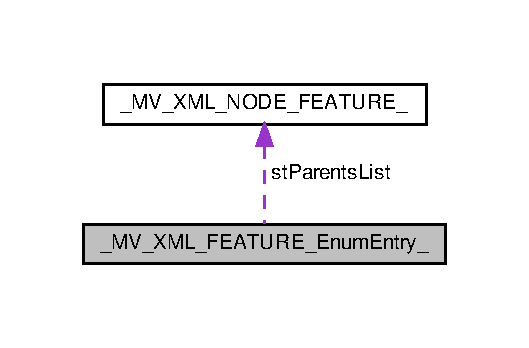
\includegraphics[width=254pt]{struct___m_v___x_m_l___f_e_a_t_u_r_e___enum_entry____coll__graph}
\end{center}
\end{figure}
\subsection*{Public 属性}
\begin{DoxyCompactItemize}
\item 
\mbox{\Hypertarget{struct___m_v___x_m_l___f_e_a_t_u_r_e___enum_entry___a06c93d8d91995c891dc8cc92b788f2ae}\label{struct___m_v___x_m_l___f_e_a_t_u_r_e___enum_entry___a06c93d8d91995c891dc8cc92b788f2ae}} 
char {\bfseries str\+Name} \mbox{[}M\+V\+\_\+\+M\+A\+X\+\_\+\+X\+M\+L\+\_\+\+N\+O\+D\+E\+\_\+\+S\+T\+R\+L\+E\+N\+\_\+C\mbox{]}
\item 
\mbox{\Hypertarget{struct___m_v___x_m_l___f_e_a_t_u_r_e___enum_entry___a38f4ed837b3d4eb2a182339adc26dc7b}\label{struct___m_v___x_m_l___f_e_a_t_u_r_e___enum_entry___a38f4ed837b3d4eb2a182339adc26dc7b}} 
char {\bfseries str\+Display\+Name} \mbox{[}M\+V\+\_\+\+M\+A\+X\+\_\+\+X\+M\+L\+\_\+\+N\+O\+D\+E\+\_\+\+S\+T\+R\+L\+E\+N\+\_\+C\mbox{]}
\item 
\mbox{\Hypertarget{struct___m_v___x_m_l___f_e_a_t_u_r_e___enum_entry___a39cef89fb45066c378d2dcde53659130}\label{struct___m_v___x_m_l___f_e_a_t_u_r_e___enum_entry___a39cef89fb45066c378d2dcde53659130}} 
char {\bfseries str\+Description} \mbox{[}M\+V\+\_\+\+M\+A\+X\+\_\+\+X\+M\+L\+\_\+\+D\+I\+S\+C\+\_\+\+S\+T\+R\+L\+E\+N\+\_\+C\mbox{]}
\item 
\mbox{\Hypertarget{struct___m_v___x_m_l___f_e_a_t_u_r_e___enum_entry___a82c2c2e12d0f1b461d09a3af478781fb}\label{struct___m_v___x_m_l___f_e_a_t_u_r_e___enum_entry___a82c2c2e12d0f1b461d09a3af478781fb}} 
char {\bfseries str\+Tool\+Tip} \mbox{[}M\+V\+\_\+\+M\+A\+X\+\_\+\+X\+M\+L\+\_\+\+D\+I\+S\+C\+\_\+\+S\+T\+R\+L\+E\+N\+\_\+C\mbox{]}
\item 
\mbox{\Hypertarget{struct___m_v___x_m_l___f_e_a_t_u_r_e___enum_entry___aff6436cb1a1dc6bb8f29e65959cf9b4a}\label{struct___m_v___x_m_l___f_e_a_t_u_r_e___enum_entry___aff6436cb1a1dc6bb8f29e65959cf9b4a}} 
int {\bfseries b\+Is\+Implemented}
\item 
\mbox{\Hypertarget{struct___m_v___x_m_l___f_e_a_t_u_r_e___enum_entry___a41dad4a487c4c3287cc1b2f94483298b}\label{struct___m_v___x_m_l___f_e_a_t_u_r_e___enum_entry___a41dad4a487c4c3287cc1b2f94483298b}} 
int {\bfseries n\+Parents\+Num}
\item 
\mbox{\Hypertarget{struct___m_v___x_m_l___f_e_a_t_u_r_e___enum_entry___a9d3d8961d4eee98656ec383210693531}\label{struct___m_v___x_m_l___f_e_a_t_u_r_e___enum_entry___a9d3d8961d4eee98656ec383210693531}} 
\hyperlink{struct___m_v___x_m_l___n_o_d_e___f_e_a_t_u_r_e__}{M\+V\+\_\+\+X\+M\+L\+\_\+\+N\+O\+D\+E\+\_\+\+F\+E\+A\+T\+U\+RE} {\bfseries st\+Parents\+List} \mbox{[}M\+V\+\_\+\+M\+A\+X\+\_\+\+X\+M\+L\+\_\+\+P\+A\+R\+E\+N\+T\+S\+\_\+\+N\+UM\mbox{]}
\item 
\mbox{\Hypertarget{struct___m_v___x_m_l___f_e_a_t_u_r_e___enum_entry___a715509bc5e33875847e035e8db3b5d72}\label{struct___m_v___x_m_l___f_e_a_t_u_r_e___enum_entry___a715509bc5e33875847e035e8db3b5d72}} 
enum M\+V\+\_\+\+X\+M\+L\+\_\+\+Visibility {\bfseries en\+Visivility}
\item 
\mbox{\Hypertarget{struct___m_v___x_m_l___f_e_a_t_u_r_e___enum_entry___ac06d3cb43097d10726f8459988fd976b}\label{struct___m_v___x_m_l___f_e_a_t_u_r_e___enum_entry___ac06d3cb43097d10726f8459988fd976b}} 
int64\+\_\+t {\bfseries n\+Value}
\item 
\mbox{\Hypertarget{struct___m_v___x_m_l___f_e_a_t_u_r_e___enum_entry___aedf5f9ec13b82975de7aea625e79de27}\label{struct___m_v___x_m_l___f_e_a_t_u_r_e___enum_entry___aedf5f9ec13b82975de7aea625e79de27}} 
enum M\+V\+\_\+\+X\+M\+L\+\_\+\+Access\+Mode {\bfseries en\+Access\+Mode}
\item 
\mbox{\Hypertarget{struct___m_v___x_m_l___f_e_a_t_u_r_e___enum_entry___a6607623c390797adef3e09d5111d940a}\label{struct___m_v___x_m_l___f_e_a_t_u_r_e___enum_entry___a6607623c390797adef3e09d5111d940a}} 
int {\bfseries b\+Is\+Locked}
\item 
\mbox{\Hypertarget{struct___m_v___x_m_l___f_e_a_t_u_r_e___enum_entry___a5511a1b4e79a50e72878687cfa9d815b}\label{struct___m_v___x_m_l___f_e_a_t_u_r_e___enum_entry___a5511a1b4e79a50e72878687cfa9d815b}} 
int {\bfseries n\+Reserved} \mbox{[}8\mbox{]}
\end{DoxyCompactItemize}


该结构体的文档由以下文件生成\+:\begin{DoxyCompactItemize}
\item 
camera/hikvision/include/Camera\+Params.\+h\end{DoxyCompactItemize}

\hypertarget{struct___m_v___x_m_l___f_e_a_t_u_r_e___enumeration__}{}\section{\+\_\+\+M\+V\+\_\+\+X\+M\+L\+\_\+\+F\+E\+A\+T\+U\+R\+E\+\_\+\+Enumeration\+\_\+结构体 参考}
\label{struct___m_v___x_m_l___f_e_a_t_u_r_e___enumeration__}\index{\+\_\+\+M\+V\+\_\+\+X\+M\+L\+\_\+\+F\+E\+A\+T\+U\+R\+E\+\_\+\+Enumeration\+\_\+@{\+\_\+\+M\+V\+\_\+\+X\+M\+L\+\_\+\+F\+E\+A\+T\+U\+R\+E\+\_\+\+Enumeration\+\_\+}}
\subsection*{Public 属性}
\begin{DoxyCompactItemize}
\item 
\mbox{\Hypertarget{struct___m_v___x_m_l___f_e_a_t_u_r_e___enumeration___ade23dc92a5dbbd6660eb72efe9976f13}\label{struct___m_v___x_m_l___f_e_a_t_u_r_e___enumeration___ade23dc92a5dbbd6660eb72efe9976f13}} 
enum M\+V\+\_\+\+X\+M\+L\+\_\+\+Visibility {\bfseries en\+Visivility}
\item 
\mbox{\Hypertarget{struct___m_v___x_m_l___f_e_a_t_u_r_e___enumeration___acdb62f655b7fc656047fe5b7dbf9e223}\label{struct___m_v___x_m_l___f_e_a_t_u_r_e___enumeration___acdb62f655b7fc656047fe5b7dbf9e223}} 
char {\bfseries str\+Description} \mbox{[}M\+V\+\_\+\+M\+A\+X\+\_\+\+X\+M\+L\+\_\+\+D\+I\+S\+C\+\_\+\+S\+T\+R\+L\+E\+N\+\_\+C\mbox{]}
\item 
\mbox{\Hypertarget{struct___m_v___x_m_l___f_e_a_t_u_r_e___enumeration___a7377a1886c39c1db69b643496d0aa325}\label{struct___m_v___x_m_l___f_e_a_t_u_r_e___enumeration___a7377a1886c39c1db69b643496d0aa325}} 
char {\bfseries str\+Display\+Name} \mbox{[}M\+V\+\_\+\+M\+A\+X\+\_\+\+X\+M\+L\+\_\+\+N\+O\+D\+E\+\_\+\+S\+T\+R\+L\+E\+N\+\_\+C\mbox{]}
\item 
\mbox{\Hypertarget{struct___m_v___x_m_l___f_e_a_t_u_r_e___enumeration___a80454fe439f794f3221001e339490d4a}\label{struct___m_v___x_m_l___f_e_a_t_u_r_e___enumeration___a80454fe439f794f3221001e339490d4a}} 
char {\bfseries str\+Name} \mbox{[}M\+V\+\_\+\+M\+A\+X\+\_\+\+X\+M\+L\+\_\+\+N\+O\+D\+E\+\_\+\+S\+T\+R\+L\+E\+N\+\_\+C\mbox{]}
\item 
\mbox{\Hypertarget{struct___m_v___x_m_l___f_e_a_t_u_r_e___enumeration___ac40e2dad99ad42b06d481b22fd20f8bb}\label{struct___m_v___x_m_l___f_e_a_t_u_r_e___enumeration___ac40e2dad99ad42b06d481b22fd20f8bb}} 
char {\bfseries str\+Tool\+Tip} \mbox{[}M\+V\+\_\+\+M\+A\+X\+\_\+\+X\+M\+L\+\_\+\+D\+I\+S\+C\+\_\+\+S\+T\+R\+L\+E\+N\+\_\+C\mbox{]}
\item 
\mbox{\Hypertarget{struct___m_v___x_m_l___f_e_a_t_u_r_e___enumeration___aee0183b12a9af6314a01cbf0789be74c}\label{struct___m_v___x_m_l___f_e_a_t_u_r_e___enumeration___aee0183b12a9af6314a01cbf0789be74c}} 
int {\bfseries n\+Symbolic\+Num}
\item 
\mbox{\Hypertarget{struct___m_v___x_m_l___f_e_a_t_u_r_e___enumeration___a03f4b71269aa86feace74fa724fbcfe9}\label{struct___m_v___x_m_l___f_e_a_t_u_r_e___enumeration___a03f4b71269aa86feace74fa724fbcfe9}} 
char {\bfseries str\+Current\+Symbolic} \mbox{[}M\+V\+\_\+\+M\+A\+X\+\_\+\+X\+M\+L\+\_\+\+S\+Y\+M\+B\+O\+L\+I\+C\+\_\+\+S\+T\+R\+L\+E\+N\+\_\+C\mbox{]}
\item 
\mbox{\Hypertarget{struct___m_v___x_m_l___f_e_a_t_u_r_e___enumeration___a47be2b0048fadb9c75305368157e7a9e}\label{struct___m_v___x_m_l___f_e_a_t_u_r_e___enumeration___a47be2b0048fadb9c75305368157e7a9e}} 
char {\bfseries str\+Symbolic} \mbox{[}M\+V\+\_\+\+M\+A\+X\+\_\+\+X\+M\+L\+\_\+\+S\+Y\+M\+B\+O\+L\+I\+C\+\_\+\+N\+UM\mbox{]}\mbox{[}M\+V\+\_\+\+M\+A\+X\+\_\+\+X\+M\+L\+\_\+\+S\+Y\+M\+B\+O\+L\+I\+C\+\_\+\+S\+T\+R\+L\+E\+N\+\_\+C\mbox{]}
\item 
\mbox{\Hypertarget{struct___m_v___x_m_l___f_e_a_t_u_r_e___enumeration___a99724e4b5c310ac673f389e1c7788a5c}\label{struct___m_v___x_m_l___f_e_a_t_u_r_e___enumeration___a99724e4b5c310ac673f389e1c7788a5c}} 
enum M\+V\+\_\+\+X\+M\+L\+\_\+\+Access\+Mode {\bfseries en\+Access\+Mode}
\item 
\mbox{\Hypertarget{struct___m_v___x_m_l___f_e_a_t_u_r_e___enumeration___a442a51aa8e6bd9be7cd1dd852b420dc0}\label{struct___m_v___x_m_l___f_e_a_t_u_r_e___enumeration___a442a51aa8e6bd9be7cd1dd852b420dc0}} 
int {\bfseries b\+Is\+Locked}
\item 
\mbox{\Hypertarget{struct___m_v___x_m_l___f_e_a_t_u_r_e___enumeration___aa54dbc48e9b171dd5109952e4df342ee}\label{struct___m_v___x_m_l___f_e_a_t_u_r_e___enumeration___aa54dbc48e9b171dd5109952e4df342ee}} 
int64\+\_\+t {\bfseries n\+Value}
\item 
\mbox{\Hypertarget{struct___m_v___x_m_l___f_e_a_t_u_r_e___enumeration___a15a412e73fb8f58027cfb0fec60b543a}\label{struct___m_v___x_m_l___f_e_a_t_u_r_e___enumeration___a15a412e73fb8f58027cfb0fec60b543a}} 
unsigned int {\bfseries n\+Reserved} \mbox{[}4\mbox{]}
\end{DoxyCompactItemize}


该结构体的文档由以下文件生成\+:\begin{DoxyCompactItemize}
\item 
camera/hikvision/include/Camera\+Params.\+h\end{DoxyCompactItemize}

\hypertarget{struct___m_v___x_m_l___f_e_a_t_u_r_e___float__}{}\section{\+\_\+\+M\+V\+\_\+\+X\+M\+L\+\_\+\+F\+E\+A\+T\+U\+R\+E\+\_\+\+Float\+\_\+结构体 参考}
\label{struct___m_v___x_m_l___f_e_a_t_u_r_e___float__}\index{\+\_\+\+M\+V\+\_\+\+X\+M\+L\+\_\+\+F\+E\+A\+T\+U\+R\+E\+\_\+\+Float\+\_\+@{\+\_\+\+M\+V\+\_\+\+X\+M\+L\+\_\+\+F\+E\+A\+T\+U\+R\+E\+\_\+\+Float\+\_\+}}
\subsection*{Public 属性}
\begin{DoxyCompactItemize}
\item 
\mbox{\Hypertarget{struct___m_v___x_m_l___f_e_a_t_u_r_e___float___a2f2287f9d08bff5657ef752dae3466f5}\label{struct___m_v___x_m_l___f_e_a_t_u_r_e___float___a2f2287f9d08bff5657ef752dae3466f5}} 
char {\bfseries str\+Name} \mbox{[}M\+V\+\_\+\+M\+A\+X\+\_\+\+X\+M\+L\+\_\+\+N\+O\+D\+E\+\_\+\+S\+T\+R\+L\+E\+N\+\_\+C\mbox{]}
\item 
\mbox{\Hypertarget{struct___m_v___x_m_l___f_e_a_t_u_r_e___float___a946c697f7b82f545c2e0cc363d61d75a}\label{struct___m_v___x_m_l___f_e_a_t_u_r_e___float___a946c697f7b82f545c2e0cc363d61d75a}} 
char {\bfseries str\+Display\+Name} \mbox{[}M\+V\+\_\+\+M\+A\+X\+\_\+\+X\+M\+L\+\_\+\+N\+O\+D\+E\+\_\+\+S\+T\+R\+L\+E\+N\+\_\+C\mbox{]}
\item 
\mbox{\Hypertarget{struct___m_v___x_m_l___f_e_a_t_u_r_e___float___a5d3e5b4fc357a625308ff1b8fe97b31e}\label{struct___m_v___x_m_l___f_e_a_t_u_r_e___float___a5d3e5b4fc357a625308ff1b8fe97b31e}} 
char {\bfseries str\+Description} \mbox{[}M\+V\+\_\+\+M\+A\+X\+\_\+\+X\+M\+L\+\_\+\+D\+I\+S\+C\+\_\+\+S\+T\+R\+L\+E\+N\+\_\+C\mbox{]}
\item 
\mbox{\Hypertarget{struct___m_v___x_m_l___f_e_a_t_u_r_e___float___a5d55c68acaba1f3cb2d5596a1c9a48c7}\label{struct___m_v___x_m_l___f_e_a_t_u_r_e___float___a5d55c68acaba1f3cb2d5596a1c9a48c7}} 
char {\bfseries str\+Tool\+Tip} \mbox{[}M\+V\+\_\+\+M\+A\+X\+\_\+\+X\+M\+L\+\_\+\+D\+I\+S\+C\+\_\+\+S\+T\+R\+L\+E\+N\+\_\+C\mbox{]}
\item 
\mbox{\Hypertarget{struct___m_v___x_m_l___f_e_a_t_u_r_e___float___a8ef8db5dde5fa55d50c29fb22cd33f46}\label{struct___m_v___x_m_l___f_e_a_t_u_r_e___float___a8ef8db5dde5fa55d50c29fb22cd33f46}} 
enum M\+V\+\_\+\+X\+M\+L\+\_\+\+Visibility {\bfseries en\+Visivility}
\item 
\mbox{\Hypertarget{struct___m_v___x_m_l___f_e_a_t_u_r_e___float___a3d4d9f7a1c76fe7240d543082534aad5}\label{struct___m_v___x_m_l___f_e_a_t_u_r_e___float___a3d4d9f7a1c76fe7240d543082534aad5}} 
enum M\+V\+\_\+\+X\+M\+L\+\_\+\+Access\+Mode {\bfseries en\+Access\+Mode}
\item 
\mbox{\Hypertarget{struct___m_v___x_m_l___f_e_a_t_u_r_e___float___ab4d498ad216e1945587d6cd09d52da88}\label{struct___m_v___x_m_l___f_e_a_t_u_r_e___float___ab4d498ad216e1945587d6cd09d52da88}} 
int {\bfseries b\+Is\+Locked}
\item 
\mbox{\Hypertarget{struct___m_v___x_m_l___f_e_a_t_u_r_e___float___ad075a5517b4dd9f1b637a87fedccd443}\label{struct___m_v___x_m_l___f_e_a_t_u_r_e___float___ad075a5517b4dd9f1b637a87fedccd443}} 
double {\bfseries df\+Value}
\item 
\mbox{\Hypertarget{struct___m_v___x_m_l___f_e_a_t_u_r_e___float___a780deed8fe406f498b214a39e5b9d04a}\label{struct___m_v___x_m_l___f_e_a_t_u_r_e___float___a780deed8fe406f498b214a39e5b9d04a}} 
double {\bfseries df\+Min\+Value}
\item 
\mbox{\Hypertarget{struct___m_v___x_m_l___f_e_a_t_u_r_e___float___a08d7aa773c86ba4d226daf300006dc8b}\label{struct___m_v___x_m_l___f_e_a_t_u_r_e___float___a08d7aa773c86ba4d226daf300006dc8b}} 
double {\bfseries df\+Max\+Value}
\item 
\mbox{\Hypertarget{struct___m_v___x_m_l___f_e_a_t_u_r_e___float___a737982c081d9e4266fee5bf1bd62913e}\label{struct___m_v___x_m_l___f_e_a_t_u_r_e___float___a737982c081d9e4266fee5bf1bd62913e}} 
double {\bfseries df\+Increment}
\item 
\mbox{\Hypertarget{struct___m_v___x_m_l___f_e_a_t_u_r_e___float___a6bb4568b34ae070ebbfedfdeac0fe51f}\label{struct___m_v___x_m_l___f_e_a_t_u_r_e___float___a6bb4568b34ae070ebbfedfdeac0fe51f}} 
unsigned int {\bfseries n\+Reserved} \mbox{[}4\mbox{]}
\end{DoxyCompactItemize}


该结构体的文档由以下文件生成\+:\begin{DoxyCompactItemize}
\item 
camera/hikvision/include/Camera\+Params.\+h\end{DoxyCompactItemize}

\hypertarget{struct___m_v___x_m_l___f_e_a_t_u_r_e___integer__}{}\section{\+\_\+\+M\+V\+\_\+\+X\+M\+L\+\_\+\+F\+E\+A\+T\+U\+R\+E\+\_\+\+Integer\+\_\+结构体 参考}
\label{struct___m_v___x_m_l___f_e_a_t_u_r_e___integer__}\index{\+\_\+\+M\+V\+\_\+\+X\+M\+L\+\_\+\+F\+E\+A\+T\+U\+R\+E\+\_\+\+Integer\+\_\+@{\+\_\+\+M\+V\+\_\+\+X\+M\+L\+\_\+\+F\+E\+A\+T\+U\+R\+E\+\_\+\+Integer\+\_\+}}
\subsection*{Public 属性}
\begin{DoxyCompactItemize}
\item 
\mbox{\Hypertarget{struct___m_v___x_m_l___f_e_a_t_u_r_e___integer___aa5907f76c6f9fbf8651189bbdda62e5e}\label{struct___m_v___x_m_l___f_e_a_t_u_r_e___integer___aa5907f76c6f9fbf8651189bbdda62e5e}} 
char {\bfseries str\+Name} \mbox{[}M\+V\+\_\+\+M\+A\+X\+\_\+\+X\+M\+L\+\_\+\+N\+O\+D\+E\+\_\+\+S\+T\+R\+L\+E\+N\+\_\+C\mbox{]}
\item 
\mbox{\Hypertarget{struct___m_v___x_m_l___f_e_a_t_u_r_e___integer___a1e86df0769aa0ce668e434b7e8f20f6e}\label{struct___m_v___x_m_l___f_e_a_t_u_r_e___integer___a1e86df0769aa0ce668e434b7e8f20f6e}} 
char {\bfseries str\+Display\+Name} \mbox{[}M\+V\+\_\+\+M\+A\+X\+\_\+\+X\+M\+L\+\_\+\+N\+O\+D\+E\+\_\+\+S\+T\+R\+L\+E\+N\+\_\+C\mbox{]}
\item 
\mbox{\Hypertarget{struct___m_v___x_m_l___f_e_a_t_u_r_e___integer___aff4b14f95a49b480b4d4d78f408372a7}\label{struct___m_v___x_m_l___f_e_a_t_u_r_e___integer___aff4b14f95a49b480b4d4d78f408372a7}} 
char {\bfseries str\+Description} \mbox{[}M\+V\+\_\+\+M\+A\+X\+\_\+\+X\+M\+L\+\_\+\+D\+I\+S\+C\+\_\+\+S\+T\+R\+L\+E\+N\+\_\+C\mbox{]}
\item 
\mbox{\Hypertarget{struct___m_v___x_m_l___f_e_a_t_u_r_e___integer___a644663321dc2ed00e9d0b0db4eafacc6}\label{struct___m_v___x_m_l___f_e_a_t_u_r_e___integer___a644663321dc2ed00e9d0b0db4eafacc6}} 
char {\bfseries str\+Tool\+Tip} \mbox{[}M\+V\+\_\+\+M\+A\+X\+\_\+\+X\+M\+L\+\_\+\+D\+I\+S\+C\+\_\+\+S\+T\+R\+L\+E\+N\+\_\+C\mbox{]}
\item 
\mbox{\Hypertarget{struct___m_v___x_m_l___f_e_a_t_u_r_e___integer___a0cbc2998c070052247066b23484b0fc2}\label{struct___m_v___x_m_l___f_e_a_t_u_r_e___integer___a0cbc2998c070052247066b23484b0fc2}} 
enum M\+V\+\_\+\+X\+M\+L\+\_\+\+Visibility {\bfseries en\+Visivility}
\item 
\mbox{\Hypertarget{struct___m_v___x_m_l___f_e_a_t_u_r_e___integer___afb74fb6279bbb4d9e5c2115694583098}\label{struct___m_v___x_m_l___f_e_a_t_u_r_e___integer___afb74fb6279bbb4d9e5c2115694583098}} 
enum M\+V\+\_\+\+X\+M\+L\+\_\+\+Access\+Mode {\bfseries en\+Access\+Mode}
\item 
\mbox{\Hypertarget{struct___m_v___x_m_l___f_e_a_t_u_r_e___integer___a87594d1743302659948c441619b706fe}\label{struct___m_v___x_m_l___f_e_a_t_u_r_e___integer___a87594d1743302659948c441619b706fe}} 
int {\bfseries b\+Is\+Locked}
\item 
\mbox{\Hypertarget{struct___m_v___x_m_l___f_e_a_t_u_r_e___integer___a4572d57481249e770a4018719d592303}\label{struct___m_v___x_m_l___f_e_a_t_u_r_e___integer___a4572d57481249e770a4018719d592303}} 
int64\+\_\+t {\bfseries n\+Value}
\item 
\mbox{\Hypertarget{struct___m_v___x_m_l___f_e_a_t_u_r_e___integer___af9468c2ea0c04c63fea7a2677cfc8dc6}\label{struct___m_v___x_m_l___f_e_a_t_u_r_e___integer___af9468c2ea0c04c63fea7a2677cfc8dc6}} 
int64\+\_\+t {\bfseries n\+Min\+Value}
\item 
\mbox{\Hypertarget{struct___m_v___x_m_l___f_e_a_t_u_r_e___integer___a265f16f955ebad28573e99855d867654}\label{struct___m_v___x_m_l___f_e_a_t_u_r_e___integer___a265f16f955ebad28573e99855d867654}} 
int64\+\_\+t {\bfseries n\+Max\+Value}
\item 
\mbox{\Hypertarget{struct___m_v___x_m_l___f_e_a_t_u_r_e___integer___a2accf8bd91888f30ef35f3c361725580}\label{struct___m_v___x_m_l___f_e_a_t_u_r_e___integer___a2accf8bd91888f30ef35f3c361725580}} 
int64\+\_\+t {\bfseries n\+Increment}
\item 
\mbox{\Hypertarget{struct___m_v___x_m_l___f_e_a_t_u_r_e___integer___a07a9e55bce050fb005949e968c6529d9}\label{struct___m_v___x_m_l___f_e_a_t_u_r_e___integer___a07a9e55bce050fb005949e968c6529d9}} 
unsigned int {\bfseries n\+Reserved} \mbox{[}4\mbox{]}
\end{DoxyCompactItemize}


该结构体的文档由以下文件生成\+:\begin{DoxyCompactItemize}
\item 
camera/hikvision/include/Camera\+Params.\+h\end{DoxyCompactItemize}

\hypertarget{struct___m_v___x_m_l___f_e_a_t_u_r_e___port__}{}\section{\+\_\+\+M\+V\+\_\+\+X\+M\+L\+\_\+\+F\+E\+A\+T\+U\+R\+E\+\_\+\+Port\+\_\+结构体 参考}
\label{struct___m_v___x_m_l___f_e_a_t_u_r_e___port__}\index{\+\_\+\+M\+V\+\_\+\+X\+M\+L\+\_\+\+F\+E\+A\+T\+U\+R\+E\+\_\+\+Port\+\_\+@{\+\_\+\+M\+V\+\_\+\+X\+M\+L\+\_\+\+F\+E\+A\+T\+U\+R\+E\+\_\+\+Port\+\_\+}}
\subsection*{Public 属性}
\begin{DoxyCompactItemize}
\item 
\mbox{\Hypertarget{struct___m_v___x_m_l___f_e_a_t_u_r_e___port___a9bc68ae0457098ca6692ab01568a604d}\label{struct___m_v___x_m_l___f_e_a_t_u_r_e___port___a9bc68ae0457098ca6692ab01568a604d}} 
enum M\+V\+\_\+\+X\+M\+L\+\_\+\+Visibility {\bfseries en\+Visivility}
\item 
\mbox{\Hypertarget{struct___m_v___x_m_l___f_e_a_t_u_r_e___port___a4a6a953433db1f886319af4db4d5c4bd}\label{struct___m_v___x_m_l___f_e_a_t_u_r_e___port___a4a6a953433db1f886319af4db4d5c4bd}} 
char {\bfseries str\+Description} \mbox{[}M\+V\+\_\+\+M\+A\+X\+\_\+\+X\+M\+L\+\_\+\+D\+I\+S\+C\+\_\+\+S\+T\+R\+L\+E\+N\+\_\+C\mbox{]}
\item 
\mbox{\Hypertarget{struct___m_v___x_m_l___f_e_a_t_u_r_e___port___a005d0c8c26aff9ace220f91ba222cfd3}\label{struct___m_v___x_m_l___f_e_a_t_u_r_e___port___a005d0c8c26aff9ace220f91ba222cfd3}} 
char {\bfseries str\+Display\+Name} \mbox{[}M\+V\+\_\+\+M\+A\+X\+\_\+\+X\+M\+L\+\_\+\+N\+O\+D\+E\+\_\+\+S\+T\+R\+L\+E\+N\+\_\+C\mbox{]}
\item 
\mbox{\Hypertarget{struct___m_v___x_m_l___f_e_a_t_u_r_e___port___ae5a5ada4b2445f0d12f3049587d99436}\label{struct___m_v___x_m_l___f_e_a_t_u_r_e___port___ae5a5ada4b2445f0d12f3049587d99436}} 
char {\bfseries str\+Name} \mbox{[}M\+V\+\_\+\+M\+A\+X\+\_\+\+X\+M\+L\+\_\+\+N\+O\+D\+E\+\_\+\+S\+T\+R\+L\+E\+N\+\_\+C\mbox{]}
\item 
\mbox{\Hypertarget{struct___m_v___x_m_l___f_e_a_t_u_r_e___port___a659a6ac74e8fd31bdd46cb94de5419fc}\label{struct___m_v___x_m_l___f_e_a_t_u_r_e___port___a659a6ac74e8fd31bdd46cb94de5419fc}} 
char {\bfseries str\+Tool\+Tip} \mbox{[}M\+V\+\_\+\+M\+A\+X\+\_\+\+X\+M\+L\+\_\+\+D\+I\+S\+C\+\_\+\+S\+T\+R\+L\+E\+N\+\_\+C\mbox{]}
\item 
\mbox{\Hypertarget{struct___m_v___x_m_l___f_e_a_t_u_r_e___port___ad5afc0f43c1790720d3f2d1d21087731}\label{struct___m_v___x_m_l___f_e_a_t_u_r_e___port___ad5afc0f43c1790720d3f2d1d21087731}} 
enum M\+V\+\_\+\+X\+M\+L\+\_\+\+Access\+Mode {\bfseries en\+Access\+Mode}
\item 
\mbox{\Hypertarget{struct___m_v___x_m_l___f_e_a_t_u_r_e___port___a0899cc485fe31d0190b4b5fec402a377}\label{struct___m_v___x_m_l___f_e_a_t_u_r_e___port___a0899cc485fe31d0190b4b5fec402a377}} 
int {\bfseries b\+Is\+Locked}
\item 
\mbox{\Hypertarget{struct___m_v___x_m_l___f_e_a_t_u_r_e___port___a42009d003d89cf2b63108b9fa48feb82}\label{struct___m_v___x_m_l___f_e_a_t_u_r_e___port___a42009d003d89cf2b63108b9fa48feb82}} 
unsigned int {\bfseries n\+Reserved} \mbox{[}4\mbox{]}
\end{DoxyCompactItemize}


该结构体的文档由以下文件生成\+:\begin{DoxyCompactItemize}
\item 
camera/hikvision/include/Camera\+Params.\+h\end{DoxyCompactItemize}

\hypertarget{struct___m_v___x_m_l___f_e_a_t_u_r_e___register__}{}\section{\+\_\+\+M\+V\+\_\+\+X\+M\+L\+\_\+\+F\+E\+A\+T\+U\+R\+E\+\_\+\+Register\+\_\+结构体 参考}
\label{struct___m_v___x_m_l___f_e_a_t_u_r_e___register__}\index{\+\_\+\+M\+V\+\_\+\+X\+M\+L\+\_\+\+F\+E\+A\+T\+U\+R\+E\+\_\+\+Register\+\_\+@{\+\_\+\+M\+V\+\_\+\+X\+M\+L\+\_\+\+F\+E\+A\+T\+U\+R\+E\+\_\+\+Register\+\_\+}}
\subsection*{Public 属性}
\begin{DoxyCompactItemize}
\item 
\mbox{\Hypertarget{struct___m_v___x_m_l___f_e_a_t_u_r_e___register___a5692444d4948b191fe5245fd067a75cf}\label{struct___m_v___x_m_l___f_e_a_t_u_r_e___register___a5692444d4948b191fe5245fd067a75cf}} 
char {\bfseries str\+Name} \mbox{[}M\+V\+\_\+\+M\+A\+X\+\_\+\+X\+M\+L\+\_\+\+N\+O\+D\+E\+\_\+\+S\+T\+R\+L\+E\+N\+\_\+C\mbox{]}
\item 
\mbox{\Hypertarget{struct___m_v___x_m_l___f_e_a_t_u_r_e___register___ad7b5b5c6eb1aec5d96f1363613ea22f8}\label{struct___m_v___x_m_l___f_e_a_t_u_r_e___register___ad7b5b5c6eb1aec5d96f1363613ea22f8}} 
char {\bfseries str\+Display\+Name} \mbox{[}M\+V\+\_\+\+M\+A\+X\+\_\+\+X\+M\+L\+\_\+\+N\+O\+D\+E\+\_\+\+S\+T\+R\+L\+E\+N\+\_\+C\mbox{]}
\item 
\mbox{\Hypertarget{struct___m_v___x_m_l___f_e_a_t_u_r_e___register___a36ecc80aaa5401f8d00a562f697e62d8}\label{struct___m_v___x_m_l___f_e_a_t_u_r_e___register___a36ecc80aaa5401f8d00a562f697e62d8}} 
char {\bfseries str\+Description} \mbox{[}M\+V\+\_\+\+M\+A\+X\+\_\+\+X\+M\+L\+\_\+\+D\+I\+S\+C\+\_\+\+S\+T\+R\+L\+E\+N\+\_\+C\mbox{]}
\item 
\mbox{\Hypertarget{struct___m_v___x_m_l___f_e_a_t_u_r_e___register___a40db457bb1765cbddd94271114d81cb6}\label{struct___m_v___x_m_l___f_e_a_t_u_r_e___register___a40db457bb1765cbddd94271114d81cb6}} 
char {\bfseries str\+Tool\+Tip} \mbox{[}M\+V\+\_\+\+M\+A\+X\+\_\+\+X\+M\+L\+\_\+\+D\+I\+S\+C\+\_\+\+S\+T\+R\+L\+E\+N\+\_\+C\mbox{]}
\item 
\mbox{\Hypertarget{struct___m_v___x_m_l___f_e_a_t_u_r_e___register___aedb1097784e1b16dce8ba113c52a82b6}\label{struct___m_v___x_m_l___f_e_a_t_u_r_e___register___aedb1097784e1b16dce8ba113c52a82b6}} 
enum M\+V\+\_\+\+X\+M\+L\+\_\+\+Visibility {\bfseries en\+Visivility}
\item 
\mbox{\Hypertarget{struct___m_v___x_m_l___f_e_a_t_u_r_e___register___a7f2258e0191aaba2c61b54529e0eff16}\label{struct___m_v___x_m_l___f_e_a_t_u_r_e___register___a7f2258e0191aaba2c61b54529e0eff16}} 
enum M\+V\+\_\+\+X\+M\+L\+\_\+\+Access\+Mode {\bfseries en\+Access\+Mode}
\item 
\mbox{\Hypertarget{struct___m_v___x_m_l___f_e_a_t_u_r_e___register___a7d6620299acedd97fbabe0f4928ab24f}\label{struct___m_v___x_m_l___f_e_a_t_u_r_e___register___a7d6620299acedd97fbabe0f4928ab24f}} 
int {\bfseries b\+Is\+Locked}
\item 
\mbox{\Hypertarget{struct___m_v___x_m_l___f_e_a_t_u_r_e___register___a5c9a352810ed4a4c85904888dcce33bf}\label{struct___m_v___x_m_l___f_e_a_t_u_r_e___register___a5c9a352810ed4a4c85904888dcce33bf}} 
int64\+\_\+t {\bfseries n\+Addr\+Value}
\item 
\mbox{\Hypertarget{struct___m_v___x_m_l___f_e_a_t_u_r_e___register___a5a7d105554fff98b158b5aaf42d8af91}\label{struct___m_v___x_m_l___f_e_a_t_u_r_e___register___a5a7d105554fff98b158b5aaf42d8af91}} 
unsigned int {\bfseries n\+Reserved} \mbox{[}4\mbox{]}
\end{DoxyCompactItemize}


该结构体的文档由以下文件生成\+:\begin{DoxyCompactItemize}
\item 
camera/hikvision/include/Camera\+Params.\+h\end{DoxyCompactItemize}

\hypertarget{struct___m_v___x_m_l___f_e_a_t_u_r_e___string__}{}\section{\+\_\+\+M\+V\+\_\+\+X\+M\+L\+\_\+\+F\+E\+A\+T\+U\+R\+E\+\_\+\+String\+\_\+结构体 参考}
\label{struct___m_v___x_m_l___f_e_a_t_u_r_e___string__}\index{\+\_\+\+M\+V\+\_\+\+X\+M\+L\+\_\+\+F\+E\+A\+T\+U\+R\+E\+\_\+\+String\+\_\+@{\+\_\+\+M\+V\+\_\+\+X\+M\+L\+\_\+\+F\+E\+A\+T\+U\+R\+E\+\_\+\+String\+\_\+}}
\subsection*{Public 属性}
\begin{DoxyCompactItemize}
\item 
\mbox{\Hypertarget{struct___m_v___x_m_l___f_e_a_t_u_r_e___string___a71344251a4fa83a92fed401189f91f46}\label{struct___m_v___x_m_l___f_e_a_t_u_r_e___string___a71344251a4fa83a92fed401189f91f46}} 
char {\bfseries str\+Name} \mbox{[}M\+V\+\_\+\+M\+A\+X\+\_\+\+X\+M\+L\+\_\+\+N\+O\+D\+E\+\_\+\+S\+T\+R\+L\+E\+N\+\_\+C\mbox{]}
\item 
\mbox{\Hypertarget{struct___m_v___x_m_l___f_e_a_t_u_r_e___string___a75604727e187138a618d3c39da75ee8d}\label{struct___m_v___x_m_l___f_e_a_t_u_r_e___string___a75604727e187138a618d3c39da75ee8d}} 
char {\bfseries str\+Display\+Name} \mbox{[}M\+V\+\_\+\+M\+A\+X\+\_\+\+X\+M\+L\+\_\+\+N\+O\+D\+E\+\_\+\+S\+T\+R\+L\+E\+N\+\_\+C\mbox{]}
\item 
\mbox{\Hypertarget{struct___m_v___x_m_l___f_e_a_t_u_r_e___string___a2bfb68e4c8f0bcef7c419dd48e98d796}\label{struct___m_v___x_m_l___f_e_a_t_u_r_e___string___a2bfb68e4c8f0bcef7c419dd48e98d796}} 
char {\bfseries str\+Description} \mbox{[}M\+V\+\_\+\+M\+A\+X\+\_\+\+X\+M\+L\+\_\+\+D\+I\+S\+C\+\_\+\+S\+T\+R\+L\+E\+N\+\_\+C\mbox{]}
\item 
\mbox{\Hypertarget{struct___m_v___x_m_l___f_e_a_t_u_r_e___string___a8fc3a87127e1673ef5165238a36401d7}\label{struct___m_v___x_m_l___f_e_a_t_u_r_e___string___a8fc3a87127e1673ef5165238a36401d7}} 
char {\bfseries str\+Tool\+Tip} \mbox{[}M\+V\+\_\+\+M\+A\+X\+\_\+\+X\+M\+L\+\_\+\+D\+I\+S\+C\+\_\+\+S\+T\+R\+L\+E\+N\+\_\+C\mbox{]}
\item 
\mbox{\Hypertarget{struct___m_v___x_m_l___f_e_a_t_u_r_e___string___a65f02b06fa8170b2791f61dd2d75f4c9}\label{struct___m_v___x_m_l___f_e_a_t_u_r_e___string___a65f02b06fa8170b2791f61dd2d75f4c9}} 
enum M\+V\+\_\+\+X\+M\+L\+\_\+\+Visibility {\bfseries en\+Visivility}
\item 
\mbox{\Hypertarget{struct___m_v___x_m_l___f_e_a_t_u_r_e___string___a0166cb764062df31ffc2a3c65d9f18f4}\label{struct___m_v___x_m_l___f_e_a_t_u_r_e___string___a0166cb764062df31ffc2a3c65d9f18f4}} 
enum M\+V\+\_\+\+X\+M\+L\+\_\+\+Access\+Mode {\bfseries en\+Access\+Mode}
\item 
\mbox{\Hypertarget{struct___m_v___x_m_l___f_e_a_t_u_r_e___string___a5f2569885e2c006d0b41d407b76899b2}\label{struct___m_v___x_m_l___f_e_a_t_u_r_e___string___a5f2569885e2c006d0b41d407b76899b2}} 
int {\bfseries b\+Is\+Locked}
\item 
\mbox{\Hypertarget{struct___m_v___x_m_l___f_e_a_t_u_r_e___string___a1771374fd47e493b07ca40f8506823f4}\label{struct___m_v___x_m_l___f_e_a_t_u_r_e___string___a1771374fd47e493b07ca40f8506823f4}} 
char {\bfseries str\+Value} \mbox{[}M\+V\+\_\+\+M\+A\+X\+\_\+\+X\+M\+L\+\_\+\+S\+T\+R\+V\+A\+L\+U\+E\+\_\+\+S\+T\+R\+L\+E\+N\+\_\+C\mbox{]}
\item 
\mbox{\Hypertarget{struct___m_v___x_m_l___f_e_a_t_u_r_e___string___aa6abfaebdd3de5325e76e562e6c6dccf}\label{struct___m_v___x_m_l___f_e_a_t_u_r_e___string___aa6abfaebdd3de5325e76e562e6c6dccf}} 
unsigned int {\bfseries n\+Reserved} \mbox{[}4\mbox{]}
\end{DoxyCompactItemize}


该结构体的文档由以下文件生成\+:\begin{DoxyCompactItemize}
\item 
camera/hikvision/include/Camera\+Params.\+h\end{DoxyCompactItemize}

\hypertarget{struct___m_v___x_m_l___f_e_a_t_u_r_e___value__}{}\section{\+\_\+\+M\+V\+\_\+\+X\+M\+L\+\_\+\+F\+E\+A\+T\+U\+R\+E\+\_\+\+Value\+\_\+结构体 参考}
\label{struct___m_v___x_m_l___f_e_a_t_u_r_e___value__}\index{\+\_\+\+M\+V\+\_\+\+X\+M\+L\+\_\+\+F\+E\+A\+T\+U\+R\+E\+\_\+\+Value\+\_\+@{\+\_\+\+M\+V\+\_\+\+X\+M\+L\+\_\+\+F\+E\+A\+T\+U\+R\+E\+\_\+\+Value\+\_\+}}
\subsection*{Public 属性}
\begin{DoxyCompactItemize}
\item 
\mbox{\Hypertarget{struct___m_v___x_m_l___f_e_a_t_u_r_e___value___a89ddd3a25d1a77e3e1942adc93676d45}\label{struct___m_v___x_m_l___f_e_a_t_u_r_e___value___a89ddd3a25d1a77e3e1942adc93676d45}} 
enum M\+V\+\_\+\+X\+M\+L\+\_\+\+Interface\+Type {\bfseries en\+Type}
\item 
\mbox{\Hypertarget{struct___m_v___x_m_l___f_e_a_t_u_r_e___value___a9bfbf4d9e5990f429bfa6f8811239c33}\label{struct___m_v___x_m_l___f_e_a_t_u_r_e___value___a9bfbf4d9e5990f429bfa6f8811239c33}} 
char {\bfseries str\+Description} \mbox{[}M\+V\+\_\+\+M\+A\+X\+\_\+\+X\+M\+L\+\_\+\+D\+I\+S\+C\+\_\+\+S\+T\+R\+L\+E\+N\+\_\+C\mbox{]}
\item 
\mbox{\Hypertarget{struct___m_v___x_m_l___f_e_a_t_u_r_e___value___a1f3e28a3a15cabe8998c31e08c364870}\label{struct___m_v___x_m_l___f_e_a_t_u_r_e___value___a1f3e28a3a15cabe8998c31e08c364870}} 
char {\bfseries str\+Display\+Name} \mbox{[}M\+V\+\_\+\+M\+A\+X\+\_\+\+X\+M\+L\+\_\+\+N\+O\+D\+E\+\_\+\+S\+T\+R\+L\+E\+N\+\_\+C\mbox{]}
\item 
\mbox{\Hypertarget{struct___m_v___x_m_l___f_e_a_t_u_r_e___value___abe34abdfa7e71a39e10ef3f46a5c010d}\label{struct___m_v___x_m_l___f_e_a_t_u_r_e___value___abe34abdfa7e71a39e10ef3f46a5c010d}} 
char {\bfseries str\+Name} \mbox{[}M\+V\+\_\+\+M\+A\+X\+\_\+\+X\+M\+L\+\_\+\+N\+O\+D\+E\+\_\+\+S\+T\+R\+L\+E\+N\+\_\+C\mbox{]}
\item 
\mbox{\Hypertarget{struct___m_v___x_m_l___f_e_a_t_u_r_e___value___af5c35f8836674787790324c2d77153b0}\label{struct___m_v___x_m_l___f_e_a_t_u_r_e___value___af5c35f8836674787790324c2d77153b0}} 
char {\bfseries str\+Tool\+Tip} \mbox{[}M\+V\+\_\+\+M\+A\+X\+\_\+\+X\+M\+L\+\_\+\+D\+I\+S\+C\+\_\+\+S\+T\+R\+L\+E\+N\+\_\+C\mbox{]}
\item 
\mbox{\Hypertarget{struct___m_v___x_m_l___f_e_a_t_u_r_e___value___a2c6c324138292b355e947b496a37307d}\label{struct___m_v___x_m_l___f_e_a_t_u_r_e___value___a2c6c324138292b355e947b496a37307d}} 
unsigned int {\bfseries n\+Reserved} \mbox{[}4\mbox{]}
\end{DoxyCompactItemize}


该结构体的文档由以下文件生成\+:\begin{DoxyCompactItemize}
\item 
camera/hikvision/include/Camera\+Params.\+h\end{DoxyCompactItemize}

\hypertarget{struct___m_v___x_m_l___n_o_d_e___f_e_a_t_u_r_e__}{}\section{\+\_\+\+M\+V\+\_\+\+X\+M\+L\+\_\+\+N\+O\+D\+E\+\_\+\+F\+E\+A\+T\+U\+R\+E\+\_\+结构体 参考}
\label{struct___m_v___x_m_l___n_o_d_e___f_e_a_t_u_r_e__}\index{\+\_\+\+M\+V\+\_\+\+X\+M\+L\+\_\+\+N\+O\+D\+E\+\_\+\+F\+E\+A\+T\+U\+R\+E\+\_\+@{\+\_\+\+M\+V\+\_\+\+X\+M\+L\+\_\+\+N\+O\+D\+E\+\_\+\+F\+E\+A\+T\+U\+R\+E\+\_\+}}
\subsection*{Public 属性}
\begin{DoxyCompactItemize}
\item 
\mbox{\Hypertarget{struct___m_v___x_m_l___n_o_d_e___f_e_a_t_u_r_e___a6cf0a595a09ecf28f526c1a2ead4627d}\label{struct___m_v___x_m_l___n_o_d_e___f_e_a_t_u_r_e___a6cf0a595a09ecf28f526c1a2ead4627d}} 
enum M\+V\+\_\+\+X\+M\+L\+\_\+\+Interface\+Type {\bfseries en\+Type}
\item 
\mbox{\Hypertarget{struct___m_v___x_m_l___n_o_d_e___f_e_a_t_u_r_e___aeda7f96cc0323f505a946317780cc628}\label{struct___m_v___x_m_l___n_o_d_e___f_e_a_t_u_r_e___aeda7f96cc0323f505a946317780cc628}} 
enum M\+V\+\_\+\+X\+M\+L\+\_\+\+Visibility {\bfseries en\+Visivility}
\item 
\mbox{\Hypertarget{struct___m_v___x_m_l___n_o_d_e___f_e_a_t_u_r_e___acf52c65e349d4075e502acfc0807e958}\label{struct___m_v___x_m_l___n_o_d_e___f_e_a_t_u_r_e___acf52c65e349d4075e502acfc0807e958}} 
char {\bfseries str\+Description} \mbox{[}M\+V\+\_\+\+M\+A\+X\+\_\+\+X\+M\+L\+\_\+\+D\+I\+S\+C\+\_\+\+S\+T\+R\+L\+E\+N\+\_\+C\mbox{]}
\item 
\mbox{\Hypertarget{struct___m_v___x_m_l___n_o_d_e___f_e_a_t_u_r_e___a7cdc452fe7d38967ecf295c114990849}\label{struct___m_v___x_m_l___n_o_d_e___f_e_a_t_u_r_e___a7cdc452fe7d38967ecf295c114990849}} 
char {\bfseries str\+Display\+Name} \mbox{[}M\+V\+\_\+\+M\+A\+X\+\_\+\+X\+M\+L\+\_\+\+N\+O\+D\+E\+\_\+\+S\+T\+R\+L\+E\+N\+\_\+C\mbox{]}
\item 
\mbox{\Hypertarget{struct___m_v___x_m_l___n_o_d_e___f_e_a_t_u_r_e___af0ac4c0554221efe72c6f990ef7e07af}\label{struct___m_v___x_m_l___n_o_d_e___f_e_a_t_u_r_e___af0ac4c0554221efe72c6f990ef7e07af}} 
char {\bfseries str\+Name} \mbox{[}M\+V\+\_\+\+M\+A\+X\+\_\+\+X\+M\+L\+\_\+\+N\+O\+D\+E\+\_\+\+S\+T\+R\+L\+E\+N\+\_\+C\mbox{]}
\item 
\mbox{\Hypertarget{struct___m_v___x_m_l___n_o_d_e___f_e_a_t_u_r_e___aab0798e063639cfef86bb79580571440}\label{struct___m_v___x_m_l___n_o_d_e___f_e_a_t_u_r_e___aab0798e063639cfef86bb79580571440}} 
char {\bfseries str\+Tool\+Tip} \mbox{[}M\+V\+\_\+\+M\+A\+X\+\_\+\+X\+M\+L\+\_\+\+D\+I\+S\+C\+\_\+\+S\+T\+R\+L\+E\+N\+\_\+C\mbox{]}
\item 
\mbox{\Hypertarget{struct___m_v___x_m_l___n_o_d_e___f_e_a_t_u_r_e___ae8ff1517622f5f655dfba8f545f2fe1e}\label{struct___m_v___x_m_l___n_o_d_e___f_e_a_t_u_r_e___ae8ff1517622f5f655dfba8f545f2fe1e}} 
unsigned int {\bfseries n\+Reserved} \mbox{[}4\mbox{]}
\end{DoxyCompactItemize}


该结构体的文档由以下文件生成\+:\begin{DoxyCompactItemize}
\item 
camera/hikvision/include/Camera\+Params.\+h\end{DoxyCompactItemize}

\hypertarget{struct___m_v___x_m_l___n_o_d_e_s___l_i_s_t__}{}\section{\+\_\+\+M\+V\+\_\+\+X\+M\+L\+\_\+\+N\+O\+D\+E\+S\+\_\+\+L\+I\+S\+T\+\_\+结构体 参考}
\label{struct___m_v___x_m_l___n_o_d_e_s___l_i_s_t__}\index{\+\_\+\+M\+V\+\_\+\+X\+M\+L\+\_\+\+N\+O\+D\+E\+S\+\_\+\+L\+I\+S\+T\+\_\+@{\+\_\+\+M\+V\+\_\+\+X\+M\+L\+\_\+\+N\+O\+D\+E\+S\+\_\+\+L\+I\+S\+T\+\_\+}}


\+\_\+\+M\+V\+\_\+\+X\+M\+L\+\_\+\+N\+O\+D\+E\+S\+\_\+\+L\+I\+S\+T\+\_\+ 的协作图\+:\nopagebreak
\begin{figure}[H]
\begin{center}
\leavevmode
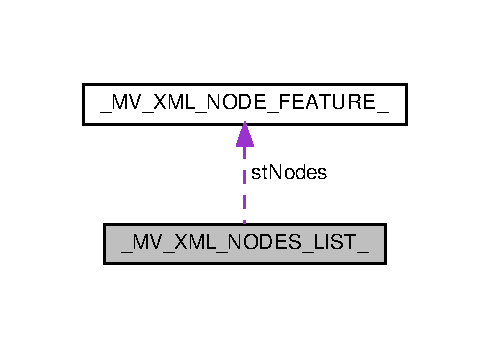
\includegraphics[width=235pt]{struct___m_v___x_m_l___n_o_d_e_s___l_i_s_t____coll__graph}
\end{center}
\end{figure}
\subsection*{Public 属性}
\begin{DoxyCompactItemize}
\item 
\mbox{\Hypertarget{struct___m_v___x_m_l___n_o_d_e_s___l_i_s_t___a1e52ea16c46b23441ba295f9e357246a}\label{struct___m_v___x_m_l___n_o_d_e_s___l_i_s_t___a1e52ea16c46b23441ba295f9e357246a}} 
unsigned int {\bfseries n\+Node\+Num}
\item 
\mbox{\Hypertarget{struct___m_v___x_m_l___n_o_d_e_s___l_i_s_t___a4e6e02432efe6b29991ceb0575739c0d}\label{struct___m_v___x_m_l___n_o_d_e_s___l_i_s_t___a4e6e02432efe6b29991ceb0575739c0d}} 
\hyperlink{struct___m_v___x_m_l___n_o_d_e___f_e_a_t_u_r_e__}{M\+V\+\_\+\+X\+M\+L\+\_\+\+N\+O\+D\+E\+\_\+\+F\+E\+A\+T\+U\+RE} {\bfseries st\+Nodes} \mbox{[}M\+V\+\_\+\+M\+A\+X\+\_\+\+X\+M\+L\+\_\+\+N\+O\+D\+E\+\_\+\+N\+U\+M\+\_\+C\mbox{]}
\end{DoxyCompactItemize}


该结构体的文档由以下文件生成\+:\begin{DoxyCompactItemize}
\item 
camera/hikvision/include/Camera\+Params.\+h\end{DoxyCompactItemize}

\hypertarget{struct___m_v_c_c___e_n_u_m_v_a_l_u_e___t}{}\section{\+\_\+\+M\+V\+C\+C\+\_\+\+E\+N\+U\+M\+V\+A\+L\+U\+E\+\_\+\+T结构体 参考}
\label{struct___m_v_c_c___e_n_u_m_v_a_l_u_e___t}\index{\+\_\+\+M\+V\+C\+C\+\_\+\+E\+N\+U\+M\+V\+A\+L\+U\+E\+\_\+T@{\+\_\+\+M\+V\+C\+C\+\_\+\+E\+N\+U\+M\+V\+A\+L\+U\+E\+\_\+T}}
\subsection*{Public 属性}
\begin{DoxyCompactItemize}
\item 
\mbox{\Hypertarget{struct___m_v_c_c___e_n_u_m_v_a_l_u_e___t_ab30f0fe7ee9b0eacf1286584bf579b4a}\label{struct___m_v_c_c___e_n_u_m_v_a_l_u_e___t_ab30f0fe7ee9b0eacf1286584bf579b4a}} 
unsigned int {\bfseries n\+Cur\+Value}
\item 
\mbox{\Hypertarget{struct___m_v_c_c___e_n_u_m_v_a_l_u_e___t_a1a43bc56d480394d927e8ded7ad94f62}\label{struct___m_v_c_c___e_n_u_m_v_a_l_u_e___t_a1a43bc56d480394d927e8ded7ad94f62}} 
unsigned int {\bfseries n\+Supported\+Num}
\item 
\mbox{\Hypertarget{struct___m_v_c_c___e_n_u_m_v_a_l_u_e___t_ac55c1e13011a2a27acfa614f76a55bf4}\label{struct___m_v_c_c___e_n_u_m_v_a_l_u_e___t_ac55c1e13011a2a27acfa614f76a55bf4}} 
unsigned int {\bfseries n\+Support\+Value} \mbox{[}M\+V\+\_\+\+M\+A\+X\+\_\+\+X\+M\+L\+\_\+\+S\+Y\+M\+B\+O\+L\+I\+C\+\_\+\+N\+UM\mbox{]}
\item 
\mbox{\Hypertarget{struct___m_v_c_c___e_n_u_m_v_a_l_u_e___t_a9cf20dd217f5450569ccebd640003fd0}\label{struct___m_v_c_c___e_n_u_m_v_a_l_u_e___t_a9cf20dd217f5450569ccebd640003fd0}} 
unsigned int {\bfseries n\+Reserved} \mbox{[}4\mbox{]}
\end{DoxyCompactItemize}


该结构体的文档由以下文件生成\+:\begin{DoxyCompactItemize}
\item 
camera/hikvision/include/Camera\+Params.\+h\end{DoxyCompactItemize}

\hypertarget{struct___m_v_c_c___f_l_o_a_t_v_a_l_u_e___t}{}\section{\+\_\+\+M\+V\+C\+C\+\_\+\+F\+L\+O\+A\+T\+V\+A\+L\+U\+E\+\_\+\+T结构体 参考}
\label{struct___m_v_c_c___f_l_o_a_t_v_a_l_u_e___t}\index{\+\_\+\+M\+V\+C\+C\+\_\+\+F\+L\+O\+A\+T\+V\+A\+L\+U\+E\+\_\+T@{\+\_\+\+M\+V\+C\+C\+\_\+\+F\+L\+O\+A\+T\+V\+A\+L\+U\+E\+\_\+T}}
\subsection*{Public 属性}
\begin{DoxyCompactItemize}
\item 
\mbox{\Hypertarget{struct___m_v_c_c___f_l_o_a_t_v_a_l_u_e___t_aaef0f2f14d594055424b8ce94c16bb61}\label{struct___m_v_c_c___f_l_o_a_t_v_a_l_u_e___t_aaef0f2f14d594055424b8ce94c16bb61}} 
float {\bfseries f\+Cur\+Value}
\item 
\mbox{\Hypertarget{struct___m_v_c_c___f_l_o_a_t_v_a_l_u_e___t_a0b296a0ce41c8c5133502335733965e0}\label{struct___m_v_c_c___f_l_o_a_t_v_a_l_u_e___t_a0b296a0ce41c8c5133502335733965e0}} 
float {\bfseries f\+Max}
\item 
\mbox{\Hypertarget{struct___m_v_c_c___f_l_o_a_t_v_a_l_u_e___t_ae8ab2c02482231ffb00374b4a9864ff7}\label{struct___m_v_c_c___f_l_o_a_t_v_a_l_u_e___t_ae8ab2c02482231ffb00374b4a9864ff7}} 
float {\bfseries f\+Min}
\item 
\mbox{\Hypertarget{struct___m_v_c_c___f_l_o_a_t_v_a_l_u_e___t_a4e7936104eddc13ccb74d8c232498fba}\label{struct___m_v_c_c___f_l_o_a_t_v_a_l_u_e___t_a4e7936104eddc13ccb74d8c232498fba}} 
unsigned int {\bfseries n\+Reserved} \mbox{[}4\mbox{]}
\end{DoxyCompactItemize}


该结构体的文档由以下文件生成\+:\begin{DoxyCompactItemize}
\item 
camera/hikvision/include/Camera\+Params.\+h\end{DoxyCompactItemize}

\hypertarget{struct___m_v_c_c___i_n_t_v_a_l_u_e___e_x___t}{}\section{\+\_\+\+M\+V\+C\+C\+\_\+\+I\+N\+T\+V\+A\+L\+U\+E\+\_\+\+E\+X\+\_\+\+T结构体 参考}
\label{struct___m_v_c_c___i_n_t_v_a_l_u_e___e_x___t}\index{\+\_\+\+M\+V\+C\+C\+\_\+\+I\+N\+T\+V\+A\+L\+U\+E\+\_\+\+E\+X\+\_\+T@{\+\_\+\+M\+V\+C\+C\+\_\+\+I\+N\+T\+V\+A\+L\+U\+E\+\_\+\+E\+X\+\_\+T}}
\subsection*{Public 属性}
\begin{DoxyCompactItemize}
\item 
\mbox{\Hypertarget{struct___m_v_c_c___i_n_t_v_a_l_u_e___e_x___t_a844c702277129fbfbb3c204db236102a}\label{struct___m_v_c_c___i_n_t_v_a_l_u_e___e_x___t_a844c702277129fbfbb3c204db236102a}} 
int64\+\_\+t {\bfseries n\+Cur\+Value}
\item 
\mbox{\Hypertarget{struct___m_v_c_c___i_n_t_v_a_l_u_e___e_x___t_aebfc13ae40868c28b801d30bcff645f2}\label{struct___m_v_c_c___i_n_t_v_a_l_u_e___e_x___t_aebfc13ae40868c28b801d30bcff645f2}} 
int64\+\_\+t {\bfseries n\+Max}
\item 
\mbox{\Hypertarget{struct___m_v_c_c___i_n_t_v_a_l_u_e___e_x___t_a14ad185c69aa175670bea0ca8abc61b9}\label{struct___m_v_c_c___i_n_t_v_a_l_u_e___e_x___t_a14ad185c69aa175670bea0ca8abc61b9}} 
int64\+\_\+t {\bfseries n\+Min}
\item 
\mbox{\Hypertarget{struct___m_v_c_c___i_n_t_v_a_l_u_e___e_x___t_aa777c930cf8fffae095c697ba9c1dfde}\label{struct___m_v_c_c___i_n_t_v_a_l_u_e___e_x___t_aa777c930cf8fffae095c697ba9c1dfde}} 
int64\+\_\+t {\bfseries n\+Inc}
\item 
\mbox{\Hypertarget{struct___m_v_c_c___i_n_t_v_a_l_u_e___e_x___t_aabfbeae728648ef82ca7f21f1ec31e60}\label{struct___m_v_c_c___i_n_t_v_a_l_u_e___e_x___t_aabfbeae728648ef82ca7f21f1ec31e60}} 
unsigned int {\bfseries n\+Reserved} \mbox{[}16\mbox{]}
\end{DoxyCompactItemize}


该结构体的文档由以下文件生成\+:\begin{DoxyCompactItemize}
\item 
camera/hikvision/include/Camera\+Params.\+h\end{DoxyCompactItemize}

\hypertarget{struct___m_v_c_c___i_n_t_v_a_l_u_e___t}{}\section{\+\_\+\+M\+V\+C\+C\+\_\+\+I\+N\+T\+V\+A\+L\+U\+E\+\_\+\+T结构体 参考}
\label{struct___m_v_c_c___i_n_t_v_a_l_u_e___t}\index{\+\_\+\+M\+V\+C\+C\+\_\+\+I\+N\+T\+V\+A\+L\+U\+E\+\_\+T@{\+\_\+\+M\+V\+C\+C\+\_\+\+I\+N\+T\+V\+A\+L\+U\+E\+\_\+T}}
\subsection*{Public 属性}
\begin{DoxyCompactItemize}
\item 
\mbox{\Hypertarget{struct___m_v_c_c___i_n_t_v_a_l_u_e___t_ab3303fadfa68e29365e0559efac6207c}\label{struct___m_v_c_c___i_n_t_v_a_l_u_e___t_ab3303fadfa68e29365e0559efac6207c}} 
unsigned int {\bfseries n\+Cur\+Value}
\item 
\mbox{\Hypertarget{struct___m_v_c_c___i_n_t_v_a_l_u_e___t_ad6df80a79082b9a8b4e6bc1610b0b7f4}\label{struct___m_v_c_c___i_n_t_v_a_l_u_e___t_ad6df80a79082b9a8b4e6bc1610b0b7f4}} 
unsigned int {\bfseries n\+Max}
\item 
\mbox{\Hypertarget{struct___m_v_c_c___i_n_t_v_a_l_u_e___t_aeb53231be87ac77e296a0b2d9a569834}\label{struct___m_v_c_c___i_n_t_v_a_l_u_e___t_aeb53231be87ac77e296a0b2d9a569834}} 
unsigned int {\bfseries n\+Min}
\item 
\mbox{\Hypertarget{struct___m_v_c_c___i_n_t_v_a_l_u_e___t_ab532f774ef137b95769dd1a90c01e55c}\label{struct___m_v_c_c___i_n_t_v_a_l_u_e___t_ab532f774ef137b95769dd1a90c01e55c}} 
unsigned int {\bfseries n\+Inc}
\item 
\mbox{\Hypertarget{struct___m_v_c_c___i_n_t_v_a_l_u_e___t_a873d765ce2257de9476450054e5d1af0}\label{struct___m_v_c_c___i_n_t_v_a_l_u_e___t_a873d765ce2257de9476450054e5d1af0}} 
unsigned int {\bfseries n\+Reserved} \mbox{[}4\mbox{]}
\end{DoxyCompactItemize}


该结构体的文档由以下文件生成\+:\begin{DoxyCompactItemize}
\item 
camera/hikvision/include/Camera\+Params.\+h\end{DoxyCompactItemize}

\hypertarget{struct___m_v_c_c___s_t_r_i_n_g_v_a_l_u_e___t}{}\section{\+\_\+\+M\+V\+C\+C\+\_\+\+S\+T\+R\+I\+N\+G\+V\+A\+L\+U\+E\+\_\+\+T结构体 参考}
\label{struct___m_v_c_c___s_t_r_i_n_g_v_a_l_u_e___t}\index{\+\_\+\+M\+V\+C\+C\+\_\+\+S\+T\+R\+I\+N\+G\+V\+A\+L\+U\+E\+\_\+T@{\+\_\+\+M\+V\+C\+C\+\_\+\+S\+T\+R\+I\+N\+G\+V\+A\+L\+U\+E\+\_\+T}}
\subsection*{Public 属性}
\begin{DoxyCompactItemize}
\item 
\mbox{\Hypertarget{struct___m_v_c_c___s_t_r_i_n_g_v_a_l_u_e___t_afd471c89b8b96d1d23097cf7ff485d43}\label{struct___m_v_c_c___s_t_r_i_n_g_v_a_l_u_e___t_afd471c89b8b96d1d23097cf7ff485d43}} 
char {\bfseries ch\+Cur\+Value} \mbox{[}256\mbox{]}
\item 
\mbox{\Hypertarget{struct___m_v_c_c___s_t_r_i_n_g_v_a_l_u_e___t_a75c6c71dc428045da06df70183ee80b2}\label{struct___m_v_c_c___s_t_r_i_n_g_v_a_l_u_e___t_a75c6c71dc428045da06df70183ee80b2}} 
int64\+\_\+t {\bfseries n\+Max\+Length}
\item 
\mbox{\Hypertarget{struct___m_v_c_c___s_t_r_i_n_g_v_a_l_u_e___t_a9d936104ce16f47ff01c533a0ed1908e}\label{struct___m_v_c_c___s_t_r_i_n_g_v_a_l_u_e___t_a9d936104ce16f47ff01c533a0ed1908e}} 
unsigned int {\bfseries n\+Reserved} \mbox{[}2\mbox{]}
\end{DoxyCompactItemize}


该结构体的文档由以下文件生成\+:\begin{DoxyCompactItemize}
\item 
camera/hikvision/include/Camera\+Params.\+h\end{DoxyCompactItemize}

\hypertarget{class_armor_detector}{}\section{Armor\+Detector类 参考}
\label{class_armor_detector}\index{Armor\+Detector@{Armor\+Detector}}
\subsection*{Public 成员函数}
\begin{DoxyCompactItemize}
\item 
\mbox{\Hypertarget{class_armor_detector_ab71ebdc57106aaf985e2f91467bd35c5}\label{class_armor_detector_ab71ebdc57106aaf985e2f91467bd35c5}} 
bool {\bfseries detect} (Mat \&src, vector$<$ \hyperlink{struct_armor_object}{Armor\+Object} $>$ \&objects)
\item 
\mbox{\Hypertarget{class_armor_detector_a2772a5e8bcce3f60eec274af2071faaf}\label{class_armor_detector_a2772a5e8bcce3f60eec274af2071faaf}} 
bool {\bfseries init\+Model} (string path)
\end{DoxyCompactItemize}


该类的文档由以下文件生成\+:\begin{DoxyCompactItemize}
\item 
detector/include/inference.\+h\item 
detector/src/inference.\+cpp\end{DoxyCompactItemize}

\hypertarget{struct_armor_object}{}\section{Armor\+Object结构体 参考}
\label{struct_armor_object}\index{Armor\+Object@{Armor\+Object}}
\subsection*{Public 属性}
\begin{DoxyCompactItemize}
\item 
\mbox{\Hypertarget{struct_armor_object_ab568e55a67ef3ab227c36fda850b512a}\label{struct_armor_object_ab568e55a67ef3ab227c36fda850b512a}} 
Point2f {\bfseries apex} \mbox{[}4\mbox{]}
\item 
\mbox{\Hypertarget{struct_armor_object_a933d6d61a8230636ee25dbec9b418fdf}\label{struct_armor_object_a933d6d61a8230636ee25dbec9b418fdf}} 
cv\+::\+Rect\+\_\+$<$ float $>$ {\bfseries rect}
\item 
\mbox{\Hypertarget{struct_armor_object_a2a1e65b74874fb58e598cf04279130b3}\label{struct_armor_object_a2a1e65b74874fb58e598cf04279130b3}} 
int {\bfseries cls}
\item 
\mbox{\Hypertarget{struct_armor_object_a5ba4deb66c6b7bf6dcb94871f4b6333b}\label{struct_armor_object_a5ba4deb66c6b7bf6dcb94871f4b6333b}} 
int {\bfseries color}
\item 
\mbox{\Hypertarget{struct_armor_object_a818c5ef90d3482b509ef4f92e695775c}\label{struct_armor_object_a818c5ef90d3482b509ef4f92e695775c}} 
int {\bfseries area}
\item 
\mbox{\Hypertarget{struct_armor_object_a111f29c27fdf2d04102c13aebb54ebef}\label{struct_armor_object_a111f29c27fdf2d04102c13aebb54ebef}} 
float {\bfseries prob}
\item 
\mbox{\Hypertarget{struct_armor_object_ad29046c851012b0bec223217fa9ab500}\label{struct_armor_object_ad29046c851012b0bec223217fa9ab500}} 
std\+::vector$<$ cv\+::\+Point2f $>$ {\bfseries pts}
\end{DoxyCompactItemize}


该结构体的文档由以下文件生成\+:\begin{DoxyCompactItemize}
\item 
detector/include/inference.\+h\end{DoxyCompactItemize}

\hypertarget{structcamera_1_1_hik_camera_1_1_camera_calibration_struct}{}\section{camera\+:\+:Hik\+Camera\+:\+:Camera\+Calibration\+Struct结构体 参考}
\label{structcamera_1_1_hik_camera_1_1_camera_calibration_struct}\index{camera\+::\+Hik\+Camera\+::\+Camera\+Calibration\+Struct@{camera\+::\+Hik\+Camera\+::\+Camera\+Calibration\+Struct}}
\subsection*{Public 属性}
\begin{DoxyCompactItemize}
\item 
\mbox{\Hypertarget{structcamera_1_1_hik_camera_1_1_camera_calibration_struct_af15661a81e14a644de17374adab21bcb}\label{structcamera_1_1_hik_camera_1_1_camera_calibration_struct_af15661a81e14a644de17374adab21bcb}} 
float {\bfseries fx}
\item 
\mbox{\Hypertarget{structcamera_1_1_hik_camera_1_1_camera_calibration_struct_ac6b53f4c349fee29af81c8aed56edb1a}\label{structcamera_1_1_hik_camera_1_1_camera_calibration_struct_ac6b53f4c349fee29af81c8aed56edb1a}} 
float {\bfseries fy}
\item 
\mbox{\Hypertarget{structcamera_1_1_hik_camera_1_1_camera_calibration_struct_a26c2681a512862a21f1904818e00ac83}\label{structcamera_1_1_hik_camera_1_1_camera_calibration_struct_a26c2681a512862a21f1904818e00ac83}} 
float {\bfseries u0}
\item 
\mbox{\Hypertarget{structcamera_1_1_hik_camera_1_1_camera_calibration_struct_ace307711dccc113b978c3a640b4aa65a}\label{structcamera_1_1_hik_camera_1_1_camera_calibration_struct_ace307711dccc113b978c3a640b4aa65a}} 
float {\bfseries v0}
\item 
\mbox{\Hypertarget{structcamera_1_1_hik_camera_1_1_camera_calibration_struct_aa0a4a147cc41ed56510c3eb208da8728}\label{structcamera_1_1_hik_camera_1_1_camera_calibration_struct_aa0a4a147cc41ed56510c3eb208da8728}} 
float {\bfseries k\+\_\+1}
\item 
\mbox{\Hypertarget{structcamera_1_1_hik_camera_1_1_camera_calibration_struct_a9bbf792ff28ba60eda29863d2416895a}\label{structcamera_1_1_hik_camera_1_1_camera_calibration_struct_a9bbf792ff28ba60eda29863d2416895a}} 
float {\bfseries k\+\_\+2}
\item 
\mbox{\Hypertarget{structcamera_1_1_hik_camera_1_1_camera_calibration_struct_ac80eb365b07ed7478ca00292e9a1fc39}\label{structcamera_1_1_hik_camera_1_1_camera_calibration_struct_ac80eb365b07ed7478ca00292e9a1fc39}} 
float {\bfseries p\+\_\+1}
\item 
\mbox{\Hypertarget{structcamera_1_1_hik_camera_1_1_camera_calibration_struct_ae3bcfd9002dd083f3c425dc59f2bfc56}\label{structcamera_1_1_hik_camera_1_1_camera_calibration_struct_ae3bcfd9002dd083f3c425dc59f2bfc56}} 
float {\bfseries p\+\_\+2}
\item 
\mbox{\Hypertarget{structcamera_1_1_hik_camera_1_1_camera_calibration_struct_ac2bf229727d84851e52fff3408bf23d3}\label{structcamera_1_1_hik_camera_1_1_camera_calibration_struct_ac2bf229727d84851e52fff3408bf23d3}} 
float {\bfseries k\+\_\+3}
\end{DoxyCompactItemize}


该结构体的文档由以下文件生成\+:\begin{DoxyCompactItemize}
\item 
camera/hikvision/include/hikvision\+\_\+camera.\+h\end{DoxyCompactItemize}

\hypertarget{struct_camera_calibration_struct}{}\section{Camera\+Calibration\+Struct结构体 参考}
\label{struct_camera_calibration_struct}\index{Camera\+Calibration\+Struct@{Camera\+Calibration\+Struct}}
\subsection*{Public 属性}
\begin{DoxyCompactItemize}
\item 
\mbox{\Hypertarget{struct_camera_calibration_struct_aab607842cfee12da0ca30135cfa4d40e}\label{struct_camera_calibration_struct_aab607842cfee12da0ca30135cfa4d40e}} 
float {\bfseries fx}
\item 
\mbox{\Hypertarget{struct_camera_calibration_struct_a64e826f02d8e8f250e38cf9838588b0c}\label{struct_camera_calibration_struct_a64e826f02d8e8f250e38cf9838588b0c}} 
float {\bfseries fy}
\item 
\mbox{\Hypertarget{struct_camera_calibration_struct_ad9e00a2e441ea50df6f599bff04fda65}\label{struct_camera_calibration_struct_ad9e00a2e441ea50df6f599bff04fda65}} 
float {\bfseries u0}
\item 
\mbox{\Hypertarget{struct_camera_calibration_struct_abcf5ea2c9c2751a7193b165685e646fa}\label{struct_camera_calibration_struct_abcf5ea2c9c2751a7193b165685e646fa}} 
float {\bfseries v0}
\item 
\mbox{\Hypertarget{struct_camera_calibration_struct_ad4f4973ef1124d17332bbe4e81e019ef}\label{struct_camera_calibration_struct_ad4f4973ef1124d17332bbe4e81e019ef}} 
float {\bfseries k\+\_\+1}
\item 
\mbox{\Hypertarget{struct_camera_calibration_struct_af77708edad9e5739f65602645410bb24}\label{struct_camera_calibration_struct_af77708edad9e5739f65602645410bb24}} 
float {\bfseries k\+\_\+2}
\item 
\mbox{\Hypertarget{struct_camera_calibration_struct_a1e101a874e0afb1f50ad7515674e1897}\label{struct_camera_calibration_struct_a1e101a874e0afb1f50ad7515674e1897}} 
float {\bfseries p\+\_\+1}
\item 
\mbox{\Hypertarget{struct_camera_calibration_struct_a4a26ba853d9db6be5510d0066e4822ae}\label{struct_camera_calibration_struct_a4a26ba853d9db6be5510d0066e4822ae}} 
float {\bfseries p\+\_\+2}
\item 
\mbox{\Hypertarget{struct_camera_calibration_struct_a1648d147d0fc13f5bd2fda572ca3838f}\label{struct_camera_calibration_struct_a1648d147d0fc13f5bd2fda572ca3838f}} 
float {\bfseries k\+\_\+3}
\end{DoxyCompactItemize}


该结构体的文档由以下文件生成\+:\begin{DoxyCompactItemize}
\item 
camera/hikvision/tool/include/calibration/camera\+Calibration.\+h\end{DoxyCompactItemize}

\hypertarget{class_c_calibration}{}\section{C\+Calibration类 参考}
\label{class_c_calibration}\index{C\+Calibration@{C\+Calibration}}
\subsection*{Public 成员函数}
\begin{DoxyCompactItemize}
\item 
\mbox{\Hypertarget{class_c_calibration_aff0a99c0b2c97d2fe1f8bed6a922ec7c}\label{class_c_calibration_aff0a99c0b2c97d2fe1f8bed6a922ec7c}} 
{\bfseries C\+Calibration} (std\+::string pattern\+Img\+Path, std\+::string calib\+Result\+Path, std\+::string cali\+Camera\+Data\+Name, std\+::string cali\+Bias\+Data\+Name, const cv\+::\+Size \&board\+Size)
\end{DoxyCompactItemize}
\subsection*{静态 Public 成员函数}
\begin{DoxyCompactItemize}
\item 
static bool \hyperlink{class_c_calibration_a07aaab95478d80eaa0eb84b6e88206f0}{camera\+Cali} ()
\item 
static \hyperlink{struct_camera_calibration_struct}{Camera\+Calibration\+Struct} \hyperlink{class_c_calibration_adb45857b39c8ec41f8dda342aa9edf2b}{read\+Calibration\+Data} (const std\+::string \&filename)
\item 
static void \hyperlink{class_c_calibration_adf452acc89ddf656d0a4cc5ab1e4d4c6}{print\+Calibration\+Data} (\hyperlink{struct_camera_calibration_struct}{Camera\+Calibration\+Struct} calibration\+Data)
\end{DoxyCompactItemize}


\subsection{成员函数说明}
\mbox{\Hypertarget{class_c_calibration_a07aaab95478d80eaa0eb84b6e88206f0}\label{class_c_calibration_a07aaab95478d80eaa0eb84b6e88206f0}} 
\index{C\+Calibration@{C\+Calibration}!camera\+Cali@{camera\+Cali}}
\index{camera\+Cali@{camera\+Cali}!C\+Calibration@{C\+Calibration}}
\subsubsection{\texorpdfstring{camera\+Cali()}{cameraCali()}}
{\footnotesize\ttfamily bool C\+Calibration\+::camera\+Cali (\begin{DoxyParamCaption}{ }\end{DoxyParamCaption})\hspace{0.3cm}{\ttfamily [static]}}

����궨 \mbox{\Hypertarget{class_c_calibration_adf452acc89ddf656d0a4cc5ab1e4d4c6}\label{class_c_calibration_adf452acc89ddf656d0a4cc5ab1e4d4c6}} 
\index{C\+Calibration@{C\+Calibration}!print\+Calibration\+Data@{print\+Calibration\+Data}}
\index{print\+Calibration\+Data@{print\+Calibration\+Data}!C\+Calibration@{C\+Calibration}}
\subsubsection{\texorpdfstring{print\+Calibration\+Data()}{printCalibrationData()}}
{\footnotesize\ttfamily void C\+Calibration\+::print\+Calibration\+Data (\begin{DoxyParamCaption}\item[{\hyperlink{struct_camera_calibration_struct}{Camera\+Calibration\+Struct}}]{calibration\+Data }\end{DoxyParamCaption})\hspace{0.3cm}{\ttfamily [static]}}

��ӡ�궨���� 
\begin{DoxyParams}{参数}
{\em calibration\+Data} & �궨�����ṹ�� \\
\hline
\end{DoxyParams}
\mbox{\Hypertarget{class_c_calibration_adb45857b39c8ec41f8dda342aa9edf2b}\label{class_c_calibration_adb45857b39c8ec41f8dda342aa9edf2b}} 
\index{C\+Calibration@{C\+Calibration}!read\+Calibration\+Data@{read\+Calibration\+Data}}
\index{read\+Calibration\+Data@{read\+Calibration\+Data}!C\+Calibration@{C\+Calibration}}
\subsubsection{\texorpdfstring{read\+Calibration\+Data()}{readCalibrationData()}}
{\footnotesize\ttfamily \hyperlink{struct_camera_calibration_struct}{Camera\+Calibration\+Struct} C\+Calibration\+::read\+Calibration\+Data (\begin{DoxyParamCaption}\item[{const std\+::string \&}]{filename }\end{DoxyParamCaption})\hspace{0.3cm}{\ttfamily [static]}}

��������궨���� 
\begin{DoxyParams}{参数}
{\em filename} & �ļ��� \\
\hline
\end{DoxyParams}
\begin{DoxyReturn}{返回}
�궨�����ṹ�� 
\end{DoxyReturn}


该类的文档由以下文件生成\+:\begin{DoxyCompactItemize}
\item 
camera/hikvision/tool/include/calibration/camera\+Calibration.\+h\item 
camera/hikvision/tool/src/calibration/camera\+Calibration.\+cpp\end{DoxyCompactItemize}

\hypertarget{class_mv_cam_ctrl_1_1_c_mv_gig_e_device}{}\section{Mv\+Cam\+Ctrl\+:\+:C\+Mv\+Gig\+E\+Device类 参考}
\label{class_mv_cam_ctrl_1_1_c_mv_gig_e_device}\index{Mv\+Cam\+Ctrl\+::\+C\+Mv\+Gig\+E\+Device@{Mv\+Cam\+Ctrl\+::\+C\+Mv\+Gig\+E\+Device}}


类 Mv\+Cam\+Ctrl\+:\+:C\+Mv\+Gig\+E\+Device 继承关系图\+:\nopagebreak
\begin{figure}[H]
\begin{center}
\leavevmode
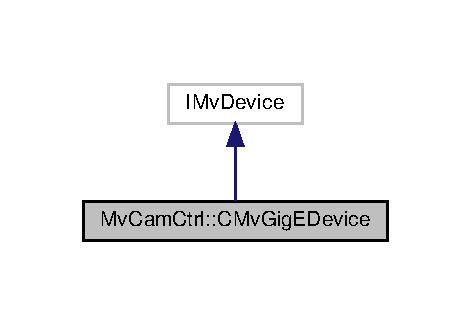
\includegraphics[width=226pt]{class_mv_cam_ctrl_1_1_c_mv_gig_e_device__inherit__graph}
\end{center}
\end{figure}


Mv\+Cam\+Ctrl\+:\+:C\+Mv\+Gig\+E\+Device 的协作图\+:\nopagebreak
\begin{figure}[H]
\begin{center}
\leavevmode
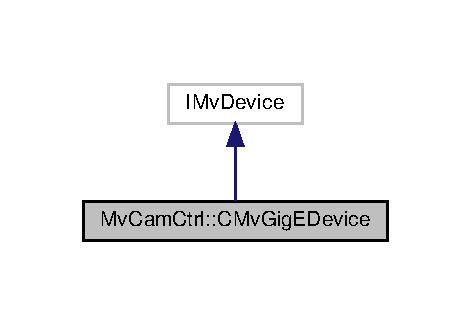
\includegraphics[width=226pt]{class_mv_cam_ctrl_1_1_c_mv_gig_e_device__coll__graph}
\end{center}
\end{figure}
\subsection*{Public 成员函数}
\begin{DoxyCompactItemize}
\item 
\mbox{\Hypertarget{class_mv_cam_ctrl_1_1_c_mv_gig_e_device_abd20873a73b3e60b0db0b885e00d2a9d}\label{class_mv_cam_ctrl_1_1_c_mv_gig_e_device_abd20873a73b3e60b0db0b885e00d2a9d}} 
virtual int {\bfseries Open} (unsigned int n\+Access\+Mode=M\+V\+\_\+\+A\+C\+C\+E\+S\+S\+\_\+\+Exclusive, unsigned short n\+Switchover\+Key=0)
\item 
\mbox{\Hypertarget{class_mv_cam_ctrl_1_1_c_mv_gig_e_device_a83a19a058f2536cdd234ed204a7b3394}\label{class_mv_cam_ctrl_1_1_c_mv_gig_e_device_a83a19a058f2536cdd234ed204a7b3394}} 
virtual int {\bfseries Close} ()
\item 
\mbox{\Hypertarget{class_mv_cam_ctrl_1_1_c_mv_gig_e_device_ab1ddefc829c3e8a3fc8e88da6d9bb803}\label{class_mv_cam_ctrl_1_1_c_mv_gig_e_device_ab1ddefc829c3e8a3fc8e88da6d9bb803}} 
virtual bool {\bfseries Is\+Open} ()
\item 
\mbox{\Hypertarget{class_mv_cam_ctrl_1_1_c_mv_gig_e_device_a8fa3303cb2232e6a9e2b9b73a161c153}\label{class_mv_cam_ctrl_1_1_c_mv_gig_e_device_a8fa3303cb2232e6a9e2b9b73a161c153}} 
virtual int {\bfseries Start\+Grabbing} ()
\item 
\mbox{\Hypertarget{class_mv_cam_ctrl_1_1_c_mv_gig_e_device_a181e57df4c02f60088af653c84732ffb}\label{class_mv_cam_ctrl_1_1_c_mv_gig_e_device_a181e57df4c02f60088af653c84732ffb}} 
virtual int {\bfseries Stop\+Grabbing} ()
\item 
\mbox{\Hypertarget{class_mv_cam_ctrl_1_1_c_mv_gig_e_device_abeaa309a6fb4bedeb3944af9b6f38428}\label{class_mv_cam_ctrl_1_1_c_mv_gig_e_device_abeaa309a6fb4bedeb3944af9b6f38428}} 
virtual int {\bfseries Get\+Device\+Info} (\hyperlink{struct___m_v___c_c___d_e_v_i_c_e___i_n_f_o__}{M\+V\+\_\+\+C\+C\+\_\+\+D\+E\+V\+I\+C\+E\+\_\+\+I\+N\+FO} \&)
\item 
virtual int \hyperlink{class_mv_cam_ctrl_1_1_c_mv_gig_e_device_a66c4c72b34394e6fe957329f47a52db2}{Get\+Gen\+I\+Cam\+X\+ML} (unsigned char $\ast$p\+Data, unsigned int n\+Data\+Size, unsigned int $\ast$pn\+Data\+Len)
\begin{DoxyCompactList}\small\item\em ��ȡ�豸��\+X\+M\+L�ļ� \end{DoxyCompactList}\item 
virtual int \hyperlink{class_mv_cam_ctrl_1_1_c_mv_gig_e_device_a0b2475f44c2b8144138cb3c47a4bc8fe}{Get\+One\+Frame} (unsigned char $\ast$p\+Data, unsigned int n\+Data\+Size, \hyperlink{struct___m_v___f_r_a_m_e___o_u_t___i_n_f_o__}{M\+V\+\_\+\+F\+R\+A\+M\+E\+\_\+\+O\+U\+T\+\_\+\+I\+N\+FO} $\ast$p\+Frame\+Info)
\begin{DoxyCompactList}\small\item\em ��ȡһ֡ͼ������ \end{DoxyCompactList}\item 
\mbox{\Hypertarget{class_mv_cam_ctrl_1_1_c_mv_gig_e_device_af3bcfdc73f64eff292de790257126fdd}\label{class_mv_cam_ctrl_1_1_c_mv_gig_e_device_af3bcfdc73f64eff292de790257126fdd}} 
virtual Tl\+Proxy {\bfseries Get\+Tl\+Proxy} ()
\item 
\mbox{\Hypertarget{class_mv_cam_ctrl_1_1_c_mv_gig_e_device_a2ce4f37e712ccc712a4ebe54ce3cb414}\label{class_mv_cam_ctrl_1_1_c_mv_gig_e_device_a2ce4f37e712ccc712a4ebe54ce3cb414}} 
{\bfseries C\+Mv\+Gig\+E\+Device} (const \hyperlink{struct___m_v___c_c___d_e_v_i_c_e___i_n_f_o__}{M\+V\+\_\+\+C\+C\+\_\+\+D\+E\+V\+I\+C\+E\+\_\+\+I\+N\+FO} $\ast$p\+Info)
\item 
\mbox{\Hypertarget{class_mv_cam_ctrl_1_1_c_mv_gig_e_device_aea9ce569fca4c4108cecdbe5e83954e3}\label{class_mv_cam_ctrl_1_1_c_mv_gig_e_device_aea9ce569fca4c4108cecdbe5e83954e3}} 
virtual int {\bfseries Get\+Net\+Trans\+Info} (\hyperlink{struct___m_v___n_e_t_t_r_a_n_s___i_n_f_o__}{M\+V\+\_\+\+N\+E\+T\+T\+R\+A\+N\+S\+\_\+\+I\+N\+FO} $\ast$pst\+Info)
\item 
\mbox{\Hypertarget{class_mv_cam_ctrl_1_1_c_mv_gig_e_device_a62cf7880cd96ba76925bfc59240b11a6}\label{class_mv_cam_ctrl_1_1_c_mv_gig_e_device_a62cf7880cd96ba76925bfc59240b11a6}} 
virtual int {\bfseries Force\+Ip} (unsigned int n\+IP)
\item 
\mbox{\Hypertarget{class_mv_cam_ctrl_1_1_c_mv_gig_e_device_aebc28e47c819a79536ac4c4d37688d69}\label{class_mv_cam_ctrl_1_1_c_mv_gig_e_device_aebc28e47c819a79536ac4c4d37688d69}} 
virtual int {\bfseries Set\+Ip\+Config} (unsigned int n\+Type)
\item 
\mbox{\Hypertarget{class_mv_cam_ctrl_1_1_c_mv_gig_e_device_a1f4209252b65612af9b2f9687e23b610}\label{class_mv_cam_ctrl_1_1_c_mv_gig_e_device_a1f4209252b65612af9b2f9687e23b610}} 
virtual int {\bfseries Get\+All\+Match\+Info} (\hyperlink{struct___m_v___a_l_l___m_a_t_c_h___i_n_f_o__}{M\+V\+\_\+\+A\+L\+L\+\_\+\+M\+A\+T\+C\+H\+\_\+\+I\+N\+FO} $\ast$pst\+Info)
\item 
\mbox{\Hypertarget{class_mv_cam_ctrl_1_1_c_mv_gig_e_device_a04334fc5f8e299ce3f36ee5478cb945a}\label{class_mv_cam_ctrl_1_1_c_mv_gig_e_device_a04334fc5f8e299ce3f36ee5478cb945a}} 
virtual int {\bfseries Register\+Exception\+Call\+Back} (void(\+\_\+\+\_\+stdcall $\ast$cb\+Exception)(unsigned int n\+Msg\+Type, void $\ast$p\+User), void $\ast$p\+User)
\item 
\mbox{\Hypertarget{class_mv_cam_ctrl_1_1_c_mv_gig_e_device_a19d05cb7da7e1bbd8cd4270ac41ad1b5}\label{class_mv_cam_ctrl_1_1_c_mv_gig_e_device_a19d05cb7da7e1bbd8cd4270ac41ad1b5}} 
virtual int {\bfseries Set\+Single\+Shot} (void(\+\_\+\+\_\+stdcall $\ast$cb\+Single\+Shot)(unsigned char $\ast$p\+Data, unsigned int n\+Data\+Len, \hyperlink{struct___m_v___f_r_a_m_e___o_u_t___i_n_f_o__}{M\+V\+\_\+\+F\+R\+A\+M\+E\+\_\+\+O\+U\+T\+\_\+\+I\+N\+FO} $\ast$p\+Frame\+Info, void $\ast$p\+User), void $\ast$p\+User)
\item 
\mbox{\Hypertarget{class_mv_cam_ctrl_1_1_c_mv_gig_e_device_a7e8d91056767cefe432427da17f8c723}\label{class_mv_cam_ctrl_1_1_c_mv_gig_e_device_a7e8d91056767cefe432427da17f8c723}} 
virtual int {\bfseries Set\+Acquisition\+Mode} (M\+V\+\_\+\+C\+A\+M\+\_\+\+A\+C\+Q\+U\+I\+S\+I\+T\+I\+O\+N\+\_\+\+M\+O\+DE en\+Mode)
\item 
\mbox{\Hypertarget{class_mv_cam_ctrl_1_1_c_mv_gig_e_device_aeb7bfc0b1e3040031661f5cdec835caa}\label{class_mv_cam_ctrl_1_1_c_mv_gig_e_device_aeb7bfc0b1e3040031661f5cdec835caa}} 
virtual int {\bfseries Local\+Upgrade} (const void $\ast$p\+File\+Path\+Name)
\item 
\mbox{\Hypertarget{class_mv_cam_ctrl_1_1_c_mv_gig_e_device_a9c5925a00191bb21539d623e3d47da58}\label{class_mv_cam_ctrl_1_1_c_mv_gig_e_device_a9c5925a00191bb21539d623e3d47da58}} 
virtual int {\bfseries Get\+Upgrade\+Process} (unsigned int $\ast$pn\+Process)
\item 
\mbox{\Hypertarget{class_mv_cam_ctrl_1_1_c_mv_gig_e_device_a39661f6b30f2e7cec1054bf361576cef}\label{class_mv_cam_ctrl_1_1_c_mv_gig_e_device_a39661f6b30f2e7cec1054bf361576cef}} 
virtual int {\bfseries Get\+Optimal\+Packet\+Size} ()
\item 
\mbox{\Hypertarget{class_mv_cam_ctrl_1_1_c_mv_gig_e_device_a3afc3e5667f9105f2915915f833cde2c}\label{class_mv_cam_ctrl_1_1_c_mv_gig_e_device_a3afc3e5667f9105f2915915f833cde2c}} 
virtual int {\bfseries Display} (void $\ast$h\+Wnd)
\item 
\mbox{\Hypertarget{class_mv_cam_ctrl_1_1_c_mv_gig_e_device_aa8e1000a46136516d73f1607d0c2b9d5}\label{class_mv_cam_ctrl_1_1_c_mv_gig_e_device_aa8e1000a46136516d73f1607d0c2b9d5}} 
virtual int {\bfseries Set\+Net\+Trans\+Mode} (unsigned int n\+Type)
\item 
\mbox{\Hypertarget{class_mv_cam_ctrl_1_1_c_mv_gig_e_device_ac702906d82ee2869ad3c2084be6474cb}\label{class_mv_cam_ctrl_1_1_c_mv_gig_e_device_ac702906d82ee2869ad3c2084be6474cb}} 
virtual int {\bfseries Read\+Memory} (void $\ast$p\+Buffer, int64\+\_\+t n\+Address, int64\+\_\+t n\+Length)
\item 
\mbox{\Hypertarget{class_mv_cam_ctrl_1_1_c_mv_gig_e_device_a0427725ce37a8caa851a51c2eda5a7b9}\label{class_mv_cam_ctrl_1_1_c_mv_gig_e_device_a0427725ce37a8caa851a51c2eda5a7b9}} 
virtual int {\bfseries Write\+Memory} (const void $\ast$p\+Buffer, int64\+\_\+t n\+Address, int64\+\_\+t n\+Length)
\item 
\mbox{\Hypertarget{class_mv_cam_ctrl_1_1_c_mv_gig_e_device_a7cd9c2d08ee18f12d48b089269a7feed}\label{class_mv_cam_ctrl_1_1_c_mv_gig_e_device_a7cd9c2d08ee18f12d48b089269a7feed}} 
virtual int {\bfseries Is\+Driver\+Working} ()
\item 
\mbox{\Hypertarget{class_mv_cam_ctrl_1_1_c_mv_gig_e_device_ad9364f4407a7cccf47358b79606b88cf}\label{class_mv_cam_ctrl_1_1_c_mv_gig_e_device_ad9364f4407a7cccf47358b79606b88cf}} 
virtual int {\bfseries Set\+Throw\+Abnormal\+Image} (int b\+Throw)
\item 
\mbox{\Hypertarget{class_mv_cam_ctrl_1_1_c_mv_gig_e_device_a5786937d1b9edc1943de7541e9da7087}\label{class_mv_cam_ctrl_1_1_c_mv_gig_e_device_a5786937d1b9edc1943de7541e9da7087}} 
virtual int {\bfseries Set\+Image\+Node\+Num} (unsigned int n\+Num)
\item 
\mbox{\Hypertarget{class_mv_cam_ctrl_1_1_c_mv_gig_e_device_a5104a9aa114676118c383472b76d80c4}\label{class_mv_cam_ctrl_1_1_c_mv_gig_e_device_a5104a9aa114676118c383472b76d80c4}} 
virtual int {\bfseries Set\+Gvcp\+Timeout} (unsigned int n\+Timeout)
\item 
\mbox{\Hypertarget{class_mv_cam_ctrl_1_1_c_mv_gig_e_device_aa8adfde56f4f46d21f3d135a02962a32}\label{class_mv_cam_ctrl_1_1_c_mv_gig_e_device_aa8adfde56f4f46d21f3d135a02962a32}} 
virtual int {\bfseries Register\+Image\+Call\+Back} (void(\+\_\+\+\_\+stdcall $\ast$cb\+Output)(unsigned char $\ast$p\+Data, \hyperlink{struct___m_v___f_r_a_m_e___o_u_t___i_n_f_o__}{M\+V\+\_\+\+F\+R\+A\+M\+E\+\_\+\+O\+U\+T\+\_\+\+I\+N\+FO} $\ast$p\+Frame\+Info, void $\ast$p\+User), void $\ast$p\+User)
\item 
\mbox{\Hypertarget{class_mv_cam_ctrl_1_1_c_mv_gig_e_device_a68d98fe75d97eef4e2cb990283d52889}\label{class_mv_cam_ctrl_1_1_c_mv_gig_e_device_a68d98fe75d97eef4e2cb990283d52889}} 
virtual int {\bfseries Register\+Event\+Call\+Back} (void(\+\_\+\+\_\+stdcall $\ast$cb\+Event)(unsigned int n\+User\+Defined\+Id, void $\ast$p\+User), void $\ast$p\+User)
\item 
\mbox{\Hypertarget{class_mv_cam_ctrl_1_1_c_mv_gig_e_device_aa9e80ab69e68c3c72c132e608ec76e17}\label{class_mv_cam_ctrl_1_1_c_mv_gig_e_device_aa9e80ab69e68c3c72c132e608ec76e17}} 
virtual int {\bfseries Register\+All\+Event\+Call\+Back} (void(\+\_\+\+\_\+stdcall $\ast$cb\+Event)(\hyperlink{struct___m_v___e_v_e_n_t___o_u_t___i_n_f_o__}{M\+V\+\_\+\+E\+V\+E\+N\+T\+\_\+\+O\+U\+T\+\_\+\+I\+N\+FO} $\ast$p\+Event\+Info, void $\ast$p\+User), void $\ast$p\+User)
\item 
\mbox{\Hypertarget{class_mv_cam_ctrl_1_1_c_mv_gig_e_device_ac595498c6f7db9a7a2d50527c84ce114}\label{class_mv_cam_ctrl_1_1_c_mv_gig_e_device_ac595498c6f7db9a7a2d50527c84ce114}} 
virtual int {\bfseries Register\+Event\+Call\+Back} (const char $\ast$p\+Event\+Name, void(\+\_\+\+\_\+stdcall $\ast$cb\+Event)(\hyperlink{struct___m_v___e_v_e_n_t___o_u_t___i_n_f_o__}{M\+V\+\_\+\+E\+V\+E\+N\+T\+\_\+\+O\+U\+T\+\_\+\+I\+N\+FO} $\ast$p\+Event\+Info, void $\ast$p\+User), void $\ast$p\+User)
\item 
\mbox{\Hypertarget{class_mv_cam_ctrl_1_1_c_mv_gig_e_device_a52099bba5546fe413264e8053cb6ca6d}\label{class_mv_cam_ctrl_1_1_c_mv_gig_e_device_a52099bba5546fe413264e8053cb6ca6d}} 
virtual int {\bfseries Register\+Image\+Call\+Back\+Ex} (void(\+\_\+\+\_\+stdcall $\ast$cb\+Output)(unsigned char $\ast$p\+Data, \hyperlink{struct___m_v___f_r_a_m_e___o_u_t___i_n_f_o___e_x__}{M\+V\+\_\+\+F\+R\+A\+M\+E\+\_\+\+O\+U\+T\+\_\+\+I\+N\+F\+O\+\_\+\+EX} $\ast$p\+Frame\+Info, void $\ast$p\+User), void $\ast$p\+User)
\item 
\mbox{\Hypertarget{class_mv_cam_ctrl_1_1_c_mv_gig_e_device_a3a874ffeda750ec9559356f7a0749e39}\label{class_mv_cam_ctrl_1_1_c_mv_gig_e_device_a3a874ffeda750ec9559356f7a0749e39}} 
virtual int {\bfseries Register\+Image\+Call\+Back\+For\+R\+GB} (void(\+\_\+\+\_\+stdcall $\ast$cb\+Output)(unsigned char $\ast$p\+Data, \hyperlink{struct___m_v___f_r_a_m_e___o_u_t___i_n_f_o___e_x__}{M\+V\+\_\+\+F\+R\+A\+M\+E\+\_\+\+O\+U\+T\+\_\+\+I\+N\+F\+O\+\_\+\+EX} $\ast$p\+Frame\+Info, void $\ast$p\+User), void $\ast$p\+User)
\item 
\mbox{\Hypertarget{class_mv_cam_ctrl_1_1_c_mv_gig_e_device_ae0b1bcb790abc15d2d34436e29ce5e60}\label{class_mv_cam_ctrl_1_1_c_mv_gig_e_device_ae0b1bcb790abc15d2d34436e29ce5e60}} 
virtual int {\bfseries Register\+Image\+Call\+Back\+For\+B\+GR} (void(\+\_\+\+\_\+stdcall $\ast$cb\+Output)(unsigned char $\ast$p\+Data, \hyperlink{struct___m_v___f_r_a_m_e___o_u_t___i_n_f_o___e_x__}{M\+V\+\_\+\+F\+R\+A\+M\+E\+\_\+\+O\+U\+T\+\_\+\+I\+N\+F\+O\+\_\+\+EX} $\ast$p\+Frame\+Info, void $\ast$p\+User), void $\ast$p\+User)
\item 
\mbox{\Hypertarget{class_mv_cam_ctrl_1_1_c_mv_gig_e_device_a226e8849efda36b6d8a6a609c3a01709}\label{class_mv_cam_ctrl_1_1_c_mv_gig_e_device_a226e8849efda36b6d8a6a609c3a01709}} 
virtual int {\bfseries Get\+One\+Frame\+Ex} (unsigned char $\ast$p\+Data, unsigned int n\+Data\+Size, \hyperlink{struct___m_v___f_r_a_m_e___o_u_t___i_n_f_o___e_x__}{M\+V\+\_\+\+F\+R\+A\+M\+E\+\_\+\+O\+U\+T\+\_\+\+I\+N\+F\+O\+\_\+\+EX} $\ast$p\+Frame\+Info)
\item 
\mbox{\Hypertarget{class_mv_cam_ctrl_1_1_c_mv_gig_e_device_a762873be03ea2dd43f832a64ff29d8ca}\label{class_mv_cam_ctrl_1_1_c_mv_gig_e_device_a762873be03ea2dd43f832a64ff29d8ca}} 
virtual int {\bfseries Get\+Image\+For\+R\+GB} (unsigned char $\ast$p\+Data, unsigned int n\+Data\+Size, \hyperlink{struct___m_v___f_r_a_m_e___o_u_t___i_n_f_o___e_x__}{M\+V\+\_\+\+F\+R\+A\+M\+E\+\_\+\+O\+U\+T\+\_\+\+I\+N\+F\+O\+\_\+\+EX} $\ast$p\+Frame\+Info, int n\+Msec)
\item 
\mbox{\Hypertarget{class_mv_cam_ctrl_1_1_c_mv_gig_e_device_aafbc12a687b1783071fe77f2cb6525fc}\label{class_mv_cam_ctrl_1_1_c_mv_gig_e_device_aafbc12a687b1783071fe77f2cb6525fc}} 
virtual int {\bfseries Get\+Image\+For\+B\+GR} (unsigned char $\ast$p\+Data, unsigned int n\+Data\+Size, \hyperlink{struct___m_v___f_r_a_m_e___o_u_t___i_n_f_o___e_x__}{M\+V\+\_\+\+F\+R\+A\+M\+E\+\_\+\+O\+U\+T\+\_\+\+I\+N\+F\+O\+\_\+\+EX} $\ast$p\+Frame\+Info, int n\+Msec)
\item 
\mbox{\Hypertarget{class_mv_cam_ctrl_1_1_c_mv_gig_e_device_a5675ebf035018cb9b09dbdc78e644f65}\label{class_mv_cam_ctrl_1_1_c_mv_gig_e_device_a5675ebf035018cb9b09dbdc78e644f65}} 
virtual int {\bfseries Get\+One\+Frame\+Timeout} (unsigned char $\ast$p\+Data, unsigned int n\+Data\+Size, \hyperlink{struct___m_v___f_r_a_m_e___o_u_t___i_n_f_o___e_x__}{M\+V\+\_\+\+F\+R\+A\+M\+E\+\_\+\+O\+U\+T\+\_\+\+I\+N\+F\+O\+\_\+\+EX} $\ast$p\+Frame\+Info, int n\+Msec)
\end{DoxyCompactItemize}


\subsection{成员函数说明}
\mbox{\Hypertarget{class_mv_cam_ctrl_1_1_c_mv_gig_e_device_a66c4c72b34394e6fe957329f47a52db2}\label{class_mv_cam_ctrl_1_1_c_mv_gig_e_device_a66c4c72b34394e6fe957329f47a52db2}} 
\index{Mv\+Cam\+Ctrl\+::\+C\+Mv\+Gig\+E\+Device@{Mv\+Cam\+Ctrl\+::\+C\+Mv\+Gig\+E\+Device}!Get\+Gen\+I\+Cam\+X\+ML@{Get\+Gen\+I\+Cam\+X\+ML}}
\index{Get\+Gen\+I\+Cam\+X\+ML@{Get\+Gen\+I\+Cam\+X\+ML}!Mv\+Cam\+Ctrl\+::\+C\+Mv\+Gig\+E\+Device@{Mv\+Cam\+Ctrl\+::\+C\+Mv\+Gig\+E\+Device}}
\subsubsection{\texorpdfstring{Get\+Gen\+I\+Cam\+X\+M\+L()}{GetGenICamXML()}}
{\footnotesize\ttfamily Mv\+Cam\+Ctrl\+::\+C\+Mv\+Gig\+E\+Device\+::\+Get\+Gen\+I\+Cam\+X\+ML (\begin{DoxyParamCaption}\item[{unsigned char $\ast$}]{p\+Data,  }\item[{unsigned int}]{n\+Data\+Size,  }\item[{unsigned int $\ast$}]{pn\+Data\+Len }\end{DoxyParamCaption})\hspace{0.3cm}{\ttfamily [virtual]}}



��ȡ�豸��\+X\+M\+L�ļ� 

Get Device X\+ML File


\begin{DoxyParams}{参数}
{\em p\+Data} & \mbox{[}IN\mbox{]}\mbox{[}O\+UT\mbox{]} -\/ ������Ļ����ַ n\+Data\+Size \mbox{[}IN\mbox{]} -\/ �����С pn\+Data\+Len \mbox{[}O\+UT\mbox{]} -\/ xml �ļ����ݳ���\\
\hline
\end{DoxyParams}
\begin{DoxyReturn}{返回}
�ɹ�������\+M\+V\+\_\+\+O\+K��ʧ�ܣ����ش����� 
\end{DoxyReturn}
\begin{DoxyNote}{注解}
��p\+DataΪ\+N\+U\+L\+L��n\+Data\+Size��ʵ�ʵ�xml�ļ�Сʱ�����������ݣ���pn\+Data\+Len����xml�ļ���С�� ��p\+DataΪ��Ч�����ַ���һ����㹻��ʱ�������������ݣ�����pn\+Data\+Len����xml�ļ���С��
\end{DoxyNote}

\begin{DoxyParams}{参数}
{\em p\+Data} & \mbox{[}IN\mbox{]}\mbox{[}O\+UT\mbox{]} -\/ Cache Address to copy in n\+Data\+Size \mbox{[}IN\mbox{]} -\/ Cache Size pn\+Data\+Len \mbox{[}O\+UT\mbox{]} -\/ X\+ML File Data Length\\
\hline
\end{DoxyParams}
\begin{DoxyReturn}{返回}
Success, return M\+V\+\_\+\+OK; Fail, return Error Code 
\end{DoxyReturn}
\begin{DoxyNote}{注解}
When p\+Data is N\+U\+LL or n\+Data\+Size is smaller than the actual xml file, do not copy data, return xml file size from the pn\+Data\+Len; When p\+Data is a valid cache address and the cache is large enough, the full data is copied and the xml file size is returned by pn\+Data\+Len. 
\end{DoxyNote}
\mbox{\Hypertarget{class_mv_cam_ctrl_1_1_c_mv_gig_e_device_a0b2475f44c2b8144138cb3c47a4bc8fe}\label{class_mv_cam_ctrl_1_1_c_mv_gig_e_device_a0b2475f44c2b8144138cb3c47a4bc8fe}} 
\index{Mv\+Cam\+Ctrl\+::\+C\+Mv\+Gig\+E\+Device@{Mv\+Cam\+Ctrl\+::\+C\+Mv\+Gig\+E\+Device}!Get\+One\+Frame@{Get\+One\+Frame}}
\index{Get\+One\+Frame@{Get\+One\+Frame}!Mv\+Cam\+Ctrl\+::\+C\+Mv\+Gig\+E\+Device@{Mv\+Cam\+Ctrl\+::\+C\+Mv\+Gig\+E\+Device}}
\subsubsection{\texorpdfstring{Get\+One\+Frame()}{GetOneFrame()}}
{\footnotesize\ttfamily Mv\+Cam\+Ctrl\+::\+C\+Mv\+Gig\+E\+Device\+::\+Get\+One\+Frame (\begin{DoxyParamCaption}\item[{unsigned char $\ast$}]{p\+Data,  }\item[{unsigned int}]{n\+Data\+Size,  }\item[{\hyperlink{struct___m_v___f_r_a_m_e___o_u_t___i_n_f_o__}{M\+V\+\_\+\+F\+R\+A\+M\+E\+\_\+\+O\+U\+T\+\_\+\+I\+N\+FO} $\ast$}]{p\+Frame\+Info }\end{DoxyParamCaption})\hspace{0.3cm}{\ttfamily [virtual]}}



��ȡһ֡ͼ������ 

Get One Frame Image Data


\begin{DoxyParams}{参数}
{\em p\+Data} & \mbox{[}IN\mbox{]}\mbox{[}O\+UT\mbox{]} -\/ ����ָ�� n\+Data\+Len \mbox{[}IN\mbox{]} -\/ ���ݳ��� p\+Frame\+Info \mbox{[}O\+UT\mbox{]} -\/ �����֡��Ϣ\\
\hline
\end{DoxyParams}
\begin{DoxyReturn}{返回}
�ɹ�������\+M\+V\+\_\+\+O\+K��ʧ�ܣ����ش�����
\end{DoxyReturn}

\begin{DoxyParams}{参数}
{\em p\+Data} & \mbox{[}IN\mbox{]}\mbox{[}O\+UT\mbox{]} -\/ Data Pointer n\+Data\+Len \mbox{[}IN\mbox{]} -\/ Data Length p\+Frame\+Info \mbox{[}O\+UT\mbox{]} -\/ Output Frame Information\\
\hline
\end{DoxyParams}
\begin{DoxyReturn}{返回}
Success, return M\+V\+\_\+\+OK; Fail, return Error Code 
\end{DoxyReturn}


该类的文档由以下文件生成\+:\begin{DoxyCompactItemize}
\item 
camera/hikvision/include/Mv\+Gig\+E\+Device.\+h\end{DoxyCompactItemize}

\hypertarget{class_mv_cam_ctrl_1_1_c_mv_usb3_v_device}{}\section{Mv\+Cam\+Ctrl\+:\+:C\+Mv\+Usb3\+V\+Device类 参考}
\label{class_mv_cam_ctrl_1_1_c_mv_usb3_v_device}\index{Mv\+Cam\+Ctrl\+::\+C\+Mv\+Usb3\+V\+Device@{Mv\+Cam\+Ctrl\+::\+C\+Mv\+Usb3\+V\+Device}}


类 Mv\+Cam\+Ctrl\+:\+:C\+Mv\+Usb3\+V\+Device 继承关系图\+:\nopagebreak
\begin{figure}[H]
\begin{center}
\leavevmode
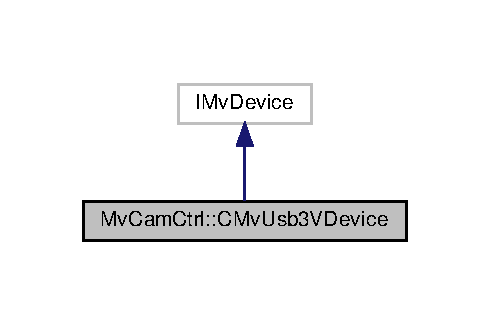
\includegraphics[width=235pt]{class_mv_cam_ctrl_1_1_c_mv_usb3_v_device__inherit__graph}
\end{center}
\end{figure}


Mv\+Cam\+Ctrl\+:\+:C\+Mv\+Usb3\+V\+Device 的协作图\+:\nopagebreak
\begin{figure}[H]
\begin{center}
\leavevmode
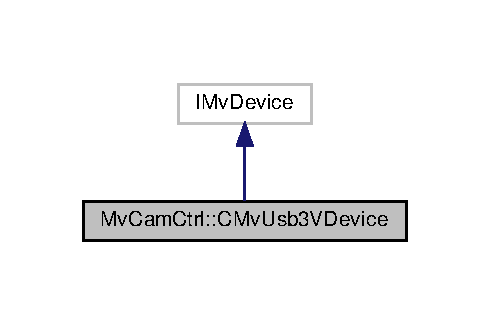
\includegraphics[width=235pt]{class_mv_cam_ctrl_1_1_c_mv_usb3_v_device__coll__graph}
\end{center}
\end{figure}
\subsection*{Public 成员函数}
\begin{DoxyCompactItemize}
\item 
\mbox{\Hypertarget{class_mv_cam_ctrl_1_1_c_mv_usb3_v_device_ae130bfdec727a1a4dc630c94d2b26c61}\label{class_mv_cam_ctrl_1_1_c_mv_usb3_v_device_ae130bfdec727a1a4dc630c94d2b26c61}} 
virtual int {\bfseries Open} (unsigned int n\+Access\+Mode=M\+V\+\_\+\+A\+C\+C\+E\+S\+S\+\_\+\+Exclusive, unsigned short n\+Switchover\+Key=0)
\item 
\mbox{\Hypertarget{class_mv_cam_ctrl_1_1_c_mv_usb3_v_device_a594c0617db698c1b7328c5b6af3597a2}\label{class_mv_cam_ctrl_1_1_c_mv_usb3_v_device_a594c0617db698c1b7328c5b6af3597a2}} 
virtual int {\bfseries Close} ()
\item 
\mbox{\Hypertarget{class_mv_cam_ctrl_1_1_c_mv_usb3_v_device_a2397e68c87d476d5a20243de23575b0d}\label{class_mv_cam_ctrl_1_1_c_mv_usb3_v_device_a2397e68c87d476d5a20243de23575b0d}} 
virtual bool {\bfseries Is\+Open} ()
\item 
\mbox{\Hypertarget{class_mv_cam_ctrl_1_1_c_mv_usb3_v_device_a1929c8752114d14d74d9b275804a7f69}\label{class_mv_cam_ctrl_1_1_c_mv_usb3_v_device_a1929c8752114d14d74d9b275804a7f69}} 
virtual int {\bfseries Start\+Grabbing} ()
\item 
\mbox{\Hypertarget{class_mv_cam_ctrl_1_1_c_mv_usb3_v_device_a94ca9b2384364e02c6b831330b9cf7f7}\label{class_mv_cam_ctrl_1_1_c_mv_usb3_v_device_a94ca9b2384364e02c6b831330b9cf7f7}} 
virtual int {\bfseries Stop\+Grabbing} ()
\item 
\mbox{\Hypertarget{class_mv_cam_ctrl_1_1_c_mv_usb3_v_device_a44e94c93ec4f0ba64528dfc5a31e7266}\label{class_mv_cam_ctrl_1_1_c_mv_usb3_v_device_a44e94c93ec4f0ba64528dfc5a31e7266}} 
virtual int {\bfseries Get\+Device\+Info} (\hyperlink{struct___m_v___c_c___d_e_v_i_c_e___i_n_f_o__}{M\+V\+\_\+\+C\+C\+\_\+\+D\+E\+V\+I\+C\+E\+\_\+\+I\+N\+FO} \&)
\item 
virtual int \hyperlink{class_mv_cam_ctrl_1_1_c_mv_usb3_v_device_a4eab362ff7dcab1c657b91492ca9afc7}{Get\+Gen\+I\+Cam\+X\+ML} (unsigned char $\ast$p\+Data, unsigned int n\+Data\+Size, unsigned int $\ast$pn\+Data\+Len)
\begin{DoxyCompactList}\small\item\em ��ȡ�豸��\+X\+M\+L�ļ� \end{DoxyCompactList}\item 
virtual int \hyperlink{class_mv_cam_ctrl_1_1_c_mv_usb3_v_device_a5c9c347b856fe38cd5651e1397c0605f}{Get\+One\+Frame} (unsigned char $\ast$p\+Data, unsigned int n\+Data\+Size, \hyperlink{struct___m_v___f_r_a_m_e___o_u_t___i_n_f_o__}{M\+V\+\_\+\+F\+R\+A\+M\+E\+\_\+\+O\+U\+T\+\_\+\+I\+N\+FO} $\ast$p\+Frame\+Info)
\begin{DoxyCompactList}\small\item\em ��ȡһ֡ͼ������ \end{DoxyCompactList}\item 
\mbox{\Hypertarget{class_mv_cam_ctrl_1_1_c_mv_usb3_v_device_a4bd76a473df25cea173da65f4e0f858f}\label{class_mv_cam_ctrl_1_1_c_mv_usb3_v_device_a4bd76a473df25cea173da65f4e0f858f}} 
virtual Tl\+Proxy {\bfseries Get\+Tl\+Proxy} ()
\item 
\mbox{\Hypertarget{class_mv_cam_ctrl_1_1_c_mv_usb3_v_device_a60c1150d7760e6afebdf8ff07b16d839}\label{class_mv_cam_ctrl_1_1_c_mv_usb3_v_device_a60c1150d7760e6afebdf8ff07b16d839}} 
{\bfseries C\+Mv\+Usb3\+V\+Device} (const \hyperlink{struct___m_v___c_c___d_e_v_i_c_e___i_n_f_o__}{M\+V\+\_\+\+C\+C\+\_\+\+D\+E\+V\+I\+C\+E\+\_\+\+I\+N\+FO} $\ast$p\+Info)
\item 
\mbox{\Hypertarget{class_mv_cam_ctrl_1_1_c_mv_usb3_v_device_a853b90012856f81f297b15df1ab2b037}\label{class_mv_cam_ctrl_1_1_c_mv_usb3_v_device_a853b90012856f81f297b15df1ab2b037}} 
virtual int {\bfseries Display} (void $\ast$h\+Wnd)
\item 
\mbox{\Hypertarget{class_mv_cam_ctrl_1_1_c_mv_usb3_v_device_aefe46f0ca60d34ec9f442977d7534d7b}\label{class_mv_cam_ctrl_1_1_c_mv_usb3_v_device_aefe46f0ca60d34ec9f442977d7534d7b}} 
virtual int {\bfseries Get\+All\+Match\+Info} (\hyperlink{struct___m_v___a_l_l___m_a_t_c_h___i_n_f_o__}{M\+V\+\_\+\+A\+L\+L\+\_\+\+M\+A\+T\+C\+H\+\_\+\+I\+N\+FO} $\ast$pst\+Info)
\item 
\mbox{\Hypertarget{class_mv_cam_ctrl_1_1_c_mv_usb3_v_device_a1c32e2fdb917dc497e19ba512ac54e1e}\label{class_mv_cam_ctrl_1_1_c_mv_usb3_v_device_a1c32e2fdb917dc497e19ba512ac54e1e}} 
virtual int {\bfseries Register\+Exception\+Call\+Back} (void(\+\_\+\+\_\+stdcall $\ast$cb\+Exception)(unsigned int n\+Msg\+Type, void $\ast$p\+User), void $\ast$p\+User)
\item 
\mbox{\Hypertarget{class_mv_cam_ctrl_1_1_c_mv_usb3_v_device_ae825122ce9a4341e329e6e964f1ece84}\label{class_mv_cam_ctrl_1_1_c_mv_usb3_v_device_ae825122ce9a4341e329e6e964f1ece84}} 
virtual int {\bfseries Set\+Single\+Shot} (void(\+\_\+\+\_\+stdcall $\ast$cb\+Single\+Shot)(unsigned char $\ast$p\+Data, unsigned int n\+Data\+Len, \hyperlink{struct___m_v___f_r_a_m_e___o_u_t___i_n_f_o__}{M\+V\+\_\+\+F\+R\+A\+M\+E\+\_\+\+O\+U\+T\+\_\+\+I\+N\+FO} $\ast$p\+Frame\+Info, void $\ast$p\+User), void $\ast$p\+User)
\item 
\mbox{\Hypertarget{class_mv_cam_ctrl_1_1_c_mv_usb3_v_device_aaeb1e9248789f328bd46d93be55b4c8f}\label{class_mv_cam_ctrl_1_1_c_mv_usb3_v_device_aaeb1e9248789f328bd46d93be55b4c8f}} 
virtual int {\bfseries Set\+Acquisition\+Mode} (M\+V\+\_\+\+C\+A\+M\+\_\+\+A\+C\+Q\+U\+I\+S\+I\+T\+I\+O\+N\+\_\+\+M\+O\+DE en\+Mode)
\item 
\mbox{\Hypertarget{class_mv_cam_ctrl_1_1_c_mv_usb3_v_device_a8d2eda057acfad39df4e0b8b72836c35}\label{class_mv_cam_ctrl_1_1_c_mv_usb3_v_device_a8d2eda057acfad39df4e0b8b72836c35}} 
virtual int {\bfseries Local\+Upgrade} (const void $\ast$p\+File\+Path\+Name)
\item 
\mbox{\Hypertarget{class_mv_cam_ctrl_1_1_c_mv_usb3_v_device_adf12cf89806e2ef6f8fc736874d19f22}\label{class_mv_cam_ctrl_1_1_c_mv_usb3_v_device_adf12cf89806e2ef6f8fc736874d19f22}} 
virtual int {\bfseries Get\+Upgrade\+Process} (unsigned int $\ast$pn\+Process)
\item 
\mbox{\Hypertarget{class_mv_cam_ctrl_1_1_c_mv_usb3_v_device_a14887209ddfaeea397d4f566e5478b34}\label{class_mv_cam_ctrl_1_1_c_mv_usb3_v_device_a14887209ddfaeea397d4f566e5478b34}} 
virtual int {\bfseries Read\+Memory} (void $\ast$p\+Buffer, int64\+\_\+t n\+Address, int64\+\_\+t n\+Length)
\item 
\mbox{\Hypertarget{class_mv_cam_ctrl_1_1_c_mv_usb3_v_device_afa32d559017bc0cf50b448aa43394364}\label{class_mv_cam_ctrl_1_1_c_mv_usb3_v_device_afa32d559017bc0cf50b448aa43394364}} 
virtual int {\bfseries Write\+Memory} (const void $\ast$p\+Buffer, int64\+\_\+t n\+Address, int64\+\_\+t n\+Length)
\item 
\mbox{\Hypertarget{class_mv_cam_ctrl_1_1_c_mv_usb3_v_device_acf853927bedd6c21bf446fe0c884228c}\label{class_mv_cam_ctrl_1_1_c_mv_usb3_v_device_acf853927bedd6c21bf446fe0c884228c}} 
virtual int {\bfseries Set\+Image\+Node\+Num} (unsigned int n\+Num)
\item 
\mbox{\Hypertarget{class_mv_cam_ctrl_1_1_c_mv_usb3_v_device_af6640ec7bf7e3d9ba00b4e970b931716}\label{class_mv_cam_ctrl_1_1_c_mv_usb3_v_device_af6640ec7bf7e3d9ba00b4e970b931716}} 
virtual int {\bfseries Register\+Image\+Call\+Back} (void(\+\_\+\+\_\+stdcall $\ast$cb\+Output)(unsigned char $\ast$p\+Data, \hyperlink{struct___m_v___f_r_a_m_e___o_u_t___i_n_f_o__}{M\+V\+\_\+\+F\+R\+A\+M\+E\+\_\+\+O\+U\+T\+\_\+\+I\+N\+FO} $\ast$p\+Frame\+Info, void $\ast$p\+User), void $\ast$p\+User)
\end{DoxyCompactItemize}


\subsection{成员函数说明}
\mbox{\Hypertarget{class_mv_cam_ctrl_1_1_c_mv_usb3_v_device_a4eab362ff7dcab1c657b91492ca9afc7}\label{class_mv_cam_ctrl_1_1_c_mv_usb3_v_device_a4eab362ff7dcab1c657b91492ca9afc7}} 
\index{Mv\+Cam\+Ctrl\+::\+C\+Mv\+Usb3\+V\+Device@{Mv\+Cam\+Ctrl\+::\+C\+Mv\+Usb3\+V\+Device}!Get\+Gen\+I\+Cam\+X\+ML@{Get\+Gen\+I\+Cam\+X\+ML}}
\index{Get\+Gen\+I\+Cam\+X\+ML@{Get\+Gen\+I\+Cam\+X\+ML}!Mv\+Cam\+Ctrl\+::\+C\+Mv\+Usb3\+V\+Device@{Mv\+Cam\+Ctrl\+::\+C\+Mv\+Usb3\+V\+Device}}
\subsubsection{\texorpdfstring{Get\+Gen\+I\+Cam\+X\+M\+L()}{GetGenICamXML()}}
{\footnotesize\ttfamily Mv\+Cam\+Ctrl\+::\+C\+Mv\+Usb3\+V\+Device\+::\+Get\+Gen\+I\+Cam\+X\+ML (\begin{DoxyParamCaption}\item[{unsigned char $\ast$}]{p\+Data,  }\item[{unsigned int}]{n\+Data\+Size,  }\item[{unsigned int $\ast$}]{pn\+Data\+Len }\end{DoxyParamCaption})\hspace{0.3cm}{\ttfamily [virtual]}}



��ȡ�豸��\+X\+M\+L�ļ� 

Get Device X\+ML Files


\begin{DoxyParams}{参数}
{\em p\+Data} & \mbox{[}IN\mbox{]}\mbox{[}O\+UT\mbox{]} -\/ ������Ļ����ַ n\+Data\+Size \mbox{[}IN\mbox{]} -\/ �����С pn\+Data\+Len \mbox{[}O\+UT\mbox{]} -\/ xml �ļ����ݳ���\\
\hline
\end{DoxyParams}
\begin{DoxyReturn}{返回}
�ɹ�������\+M\+V\+\_\+\+O\+K��ʧ�ܣ����ش����� 
\end{DoxyReturn}
\begin{DoxyNote}{注解}
��p\+DataΪ\+N\+U\+L\+L��n\+Data\+Size��ʵ�ʵ�xml�ļ�Сʱ�����������ݣ���pn\+Data\+Len����xml�ļ���С�� ��p\+DataΪ��Ч�����ַ���һ����㹻��ʱ�������������ݣ�����pn\+Data\+Len����xml�ļ���С��
\end{DoxyNote}

\begin{DoxyParams}{参数}
{\em p\+Data} & \mbox{[}IN\mbox{]}\mbox{[}O\+UT\mbox{]} -\/ Cache Address to copy in n\+Data\+Size \mbox{[}IN\mbox{]} -\/ Cache Size pn\+Data\+Len \mbox{[}O\+UT\mbox{]} -\/ X\+ML File Data Length\\
\hline
\end{DoxyParams}
\begin{DoxyReturn}{返回}
Success, return M\+V\+\_\+\+OK; Fail, return Error Code 
\end{DoxyReturn}
\begin{DoxyNote}{注解}
When p\+Data is N\+U\+LL or n\+Data\+Size is smaller than the actual xml file, do not copy data, return xml file size from the pn\+Data\+Len; When p\+Data is a valid cache address and the cache is large enough, the full data is copied and the xml file size is returned by pn\+Data\+Len. 
\end{DoxyNote}
\mbox{\Hypertarget{class_mv_cam_ctrl_1_1_c_mv_usb3_v_device_a5c9c347b856fe38cd5651e1397c0605f}\label{class_mv_cam_ctrl_1_1_c_mv_usb3_v_device_a5c9c347b856fe38cd5651e1397c0605f}} 
\index{Mv\+Cam\+Ctrl\+::\+C\+Mv\+Usb3\+V\+Device@{Mv\+Cam\+Ctrl\+::\+C\+Mv\+Usb3\+V\+Device}!Get\+One\+Frame@{Get\+One\+Frame}}
\index{Get\+One\+Frame@{Get\+One\+Frame}!Mv\+Cam\+Ctrl\+::\+C\+Mv\+Usb3\+V\+Device@{Mv\+Cam\+Ctrl\+::\+C\+Mv\+Usb3\+V\+Device}}
\subsubsection{\texorpdfstring{Get\+One\+Frame()}{GetOneFrame()}}
{\footnotesize\ttfamily Mv\+Cam\+Ctrl\+::\+C\+Mv\+Usb3\+V\+Device\+::\+Get\+One\+Frame (\begin{DoxyParamCaption}\item[{unsigned char $\ast$}]{p\+Data,  }\item[{unsigned int}]{n\+Data\+Size,  }\item[{\hyperlink{struct___m_v___f_r_a_m_e___o_u_t___i_n_f_o__}{M\+V\+\_\+\+F\+R\+A\+M\+E\+\_\+\+O\+U\+T\+\_\+\+I\+N\+FO} $\ast$}]{p\+Frame\+Info }\end{DoxyParamCaption})\hspace{0.3cm}{\ttfamily [virtual]}}



��ȡһ֡ͼ������ 

Get One Frame Image Data


\begin{DoxyParams}{参数}
{\em p\+Data} & \mbox{[}IN\mbox{]}\mbox{[}O\+UT\mbox{]} -\/ ����ָ�� n\+Data\+Len \mbox{[}IN\mbox{]} -\/ ���ݳ��� p\+Frame\+Info \mbox{[}O\+UT\mbox{]} -\/ �����֡��Ϣ\\
\hline
\end{DoxyParams}
\begin{DoxyReturn}{返回}
�ɹ�������\+M\+V\+\_\+\+O\+K��ʧ�ܣ����ش�����
\end{DoxyReturn}

\begin{DoxyParams}{参数}
{\em p\+Data} & \mbox{[}IN\mbox{]}\mbox{[}O\+UT\mbox{]} -\/ Data Pointer n\+Data\+Len \mbox{[}IN\mbox{]} -\/ Data Length p\+Frame\+Info \mbox{[}O\+UT\mbox{]} -\/ Output Frame Information\\
\hline
\end{DoxyParams}
\begin{DoxyReturn}{返回}
Success, return M\+V\+\_\+\+OK; Fail, return Error Code 
\end{DoxyReturn}


该类的文档由以下文件生成\+:\begin{DoxyCompactItemize}
\item 
camera/hikvision/include/Mv\+Usb3\+V\+Device.\+h\end{DoxyCompactItemize}

\hypertarget{class_mv_cam_ctrl_1_1_c_tl_factory}{}\section{Mv\+Cam\+Ctrl\+:\+:C\+Tl\+Factory类 参考}
\label{class_mv_cam_ctrl_1_1_c_tl_factory}\index{Mv\+Cam\+Ctrl\+::\+C\+Tl\+Factory@{Mv\+Cam\+Ctrl\+::\+C\+Tl\+Factory}}


类 Mv\+Cam\+Ctrl\+:\+:C\+Tl\+Factory 继承关系图\+:\nopagebreak
\begin{figure}[H]
\begin{center}
\leavevmode
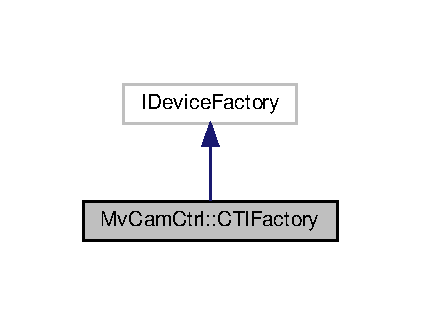
\includegraphics[width=202pt]{class_mv_cam_ctrl_1_1_c_tl_factory__inherit__graph}
\end{center}
\end{figure}


Mv\+Cam\+Ctrl\+:\+:C\+Tl\+Factory 的协作图\+:\nopagebreak
\begin{figure}[H]
\begin{center}
\leavevmode
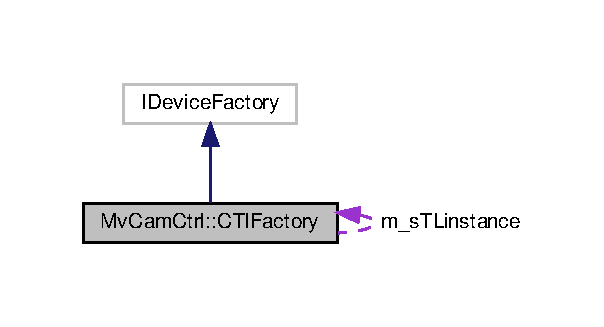
\includegraphics[width=290pt]{class_mv_cam_ctrl_1_1_c_tl_factory__coll__graph}
\end{center}
\end{figure}
\subsection*{Public 成员函数}
\begin{DoxyCompactItemize}
\item 
\mbox{\Hypertarget{class_mv_cam_ctrl_1_1_c_tl_factory_ad870bf303f7b2da875a9d8b965812456}\label{class_mv_cam_ctrl_1_1_c_tl_factory_ad870bf303f7b2da875a9d8b965812456}} 
unsigned int \hyperlink{class_mv_cam_ctrl_1_1_c_tl_factory_ad870bf303f7b2da875a9d8b965812456}{Enumerate\+Tls} ()
\begin{DoxyCompactList}\small\item\em Retrieve all available transport layers \end{DoxyCompactList}\item 
virtual int \hyperlink{class_mv_cam_ctrl_1_1_c_tl_factory_a9f57ef147a838171da7ffcbcf5b81f2e}{Enum\+Devices} (unsigned int n\+T\+Layer\+Type, \hyperlink{struct___m_v___c_c___d_e_v_i_c_e___i_n_f_o___l_i_s_t__}{M\+V\+\_\+\+C\+C\+\_\+\+D\+E\+V\+I\+C\+E\+\_\+\+I\+N\+F\+O\+\_\+\+L\+I\+ST} \&st\+Dev\+List)
\begin{DoxyCompactList}\small\item\em ö�������ڣ�ָ���Ĵ���Э���Ӧ�������豸 \end{DoxyCompactList}\item 
virtual I\+Mv\+Device $\ast$ \hyperlink{class_mv_cam_ctrl_1_1_c_tl_factory_a0fb52c7a6e1e9fff982f71039d163066}{Create\+Device} (const \hyperlink{struct___m_v___c_c___d_e_v_i_c_e___i_n_f_o__}{M\+V\+\_\+\+C\+C\+\_\+\+D\+E\+V\+I\+C\+E\+\_\+\+I\+N\+FO} \&device)
\begin{DoxyCompactList}\small\item\em �����豸������ \end{DoxyCompactList}\item 
virtual int \hyperlink{class_mv_cam_ctrl_1_1_c_tl_factory_aa3526fac869bd0cd057749ab6675fb42}{Destroy\+Device} (I\+Mv\+Device $\ast$)
\begin{DoxyCompactList}\small\item\em ����ָ���豸���ڲ���Դ \end{DoxyCompactList}\item 
virtual bool \hyperlink{class_mv_cam_ctrl_1_1_c_tl_factory_aeba5eb53746a557fbbc663fb36e101ba}{Is\+Device\+Accessible} (const \hyperlink{struct___m_v___c_c___d_e_v_i_c_e___i_n_f_o__}{M\+V\+\_\+\+C\+C\+\_\+\+D\+E\+V\+I\+C\+E\+\_\+\+I\+N\+FO} \&device\+Info)
\begin{DoxyCompactList}\small\item\em �ж�ָ�����豸�Ƿ���Է��� \end{DoxyCompactList}\item 
\mbox{\Hypertarget{class_mv_cam_ctrl_1_1_c_tl_factory_a10cfe8343a10b1c1c2f989b9ea38d6de}\label{class_mv_cam_ctrl_1_1_c_tl_factory_a10cfe8343a10b1c1c2f989b9ea38d6de}} 
virtual unsigned int {\bfseries Get\+S\+D\+K\+Version} ()
\end{DoxyCompactItemize}
\subsection*{静态 Public 成员函数}
\begin{DoxyCompactItemize}
\item 
\mbox{\Hypertarget{class_mv_cam_ctrl_1_1_c_tl_factory_ab948b0e9c91d65271d84c832ac7e1385}\label{class_mv_cam_ctrl_1_1_c_tl_factory_ab948b0e9c91d65271d84c832ac7e1385}} 
static \hyperlink{class_mv_cam_ctrl_1_1_c_tl_factory}{C\+Tl\+Factory} \& \hyperlink{class_mv_cam_ctrl_1_1_c_tl_factory_ab948b0e9c91d65271d84c832ac7e1385}{Get\+Instance} ()
\begin{DoxyCompactList}\small\item\em Retrieve the transport layer factory singleton \end{DoxyCompactList}\end{DoxyCompactItemize}
\subsection*{Protected 属性}
\begin{DoxyCompactItemize}
\item 
\mbox{\Hypertarget{class_mv_cam_ctrl_1_1_c_tl_factory_a4a0abd5141d1da5b01671686dbfe8b3a}\label{class_mv_cam_ctrl_1_1_c_tl_factory_a4a0abd5141d1da5b01671686dbfe8b3a}} 
Gen\+Api\+::\+C\+Lock {\bfseries m\+\_\+c\+Lock}
\item 
\mbox{\Hypertarget{class_mv_cam_ctrl_1_1_c_tl_factory_a07409d126d37e8d20ae5e0bd7e96f1f4}\label{class_mv_cam_ctrl_1_1_c_tl_factory_a07409d126d37e8d20ae5e0bd7e96f1f4}} 
C\+Tl\+Refs $\ast$ {\bfseries m\+\_\+p\+Created\+Tls}
\end{DoxyCompactItemize}
\subsection*{静态 Protected 属性}
\begin{DoxyCompactItemize}
\item 
\mbox{\Hypertarget{class_mv_cam_ctrl_1_1_c_tl_factory_a460e6710e7d13a4663551f4e6cf807df}\label{class_mv_cam_ctrl_1_1_c_tl_factory_a460e6710e7d13a4663551f4e6cf807df}} 
static \hyperlink{class_mv_cam_ctrl_1_1_c_tl_factory}{C\+Tl\+Factory} {\bfseries m\+\_\+s\+T\+Linstance}
\end{DoxyCompactItemize}


\subsection{成员函数说明}
\mbox{\Hypertarget{class_mv_cam_ctrl_1_1_c_tl_factory_a0fb52c7a6e1e9fff982f71039d163066}\label{class_mv_cam_ctrl_1_1_c_tl_factory_a0fb52c7a6e1e9fff982f71039d163066}} 
\index{Mv\+Cam\+Ctrl\+::\+C\+Tl\+Factory@{Mv\+Cam\+Ctrl\+::\+C\+Tl\+Factory}!Create\+Device@{Create\+Device}}
\index{Create\+Device@{Create\+Device}!Mv\+Cam\+Ctrl\+::\+C\+Tl\+Factory@{Mv\+Cam\+Ctrl\+::\+C\+Tl\+Factory}}
\subsubsection{\texorpdfstring{Create\+Device()}{CreateDevice()}}
{\footnotesize\ttfamily Mv\+Cam\+Ctrl\+::\+C\+Tl\+Factory\+::\+Create\+Device (\begin{DoxyParamCaption}\item[{const \hyperlink{struct___m_v___c_c___d_e_v_i_c_e___i_n_f_o__}{M\+V\+\_\+\+C\+C\+\_\+\+D\+E\+V\+I\+C\+E\+\_\+\+I\+N\+FO} \&}]{device }\end{DoxyParamCaption})\hspace{0.3cm}{\ttfamily [virtual]}}



�����豸������ 

Create Device Agent Class


\begin{DoxyParams}{参数}
{\em device} & \mbox{[}IN\mbox{]} -\/ �豸��Ϣ����Ҫ�����������Ч���ɣ�\\
\hline
\end{DoxyParams}
\begin{DoxyReturn}{返回}
�ɹ��������豸����ʵ����ʧ�ܣ�����\+N\+U\+LL
\end{DoxyReturn}

\begin{DoxyParams}{参数}
{\em device} & \mbox{[}IN\mbox{]} -\/ Device Information��\+Only the transport layer type valid is required��\\
\hline
\end{DoxyParams}
\begin{DoxyReturn}{返回}
Success, return device agent instance; Fail, return N\+U\+LL 
\end{DoxyReturn}
\mbox{\Hypertarget{class_mv_cam_ctrl_1_1_c_tl_factory_aa3526fac869bd0cd057749ab6675fb42}\label{class_mv_cam_ctrl_1_1_c_tl_factory_aa3526fac869bd0cd057749ab6675fb42}} 
\index{Mv\+Cam\+Ctrl\+::\+C\+Tl\+Factory@{Mv\+Cam\+Ctrl\+::\+C\+Tl\+Factory}!Destroy\+Device@{Destroy\+Device}}
\index{Destroy\+Device@{Destroy\+Device}!Mv\+Cam\+Ctrl\+::\+C\+Tl\+Factory@{Mv\+Cam\+Ctrl\+::\+C\+Tl\+Factory}}
\subsubsection{\texorpdfstring{Destroy\+Device()}{DestroyDevice()}}
{\footnotesize\ttfamily Mv\+Cam\+Ctrl\+::\+C\+Tl\+Factory\+::\+Destroy\+Device (\begin{DoxyParamCaption}\item[{I\+Mv\+Device $\ast$}]{p\+Device }\end{DoxyParamCaption})\hspace{0.3cm}{\ttfamily [virtual]}}



����ָ���豸���ڲ���Դ 

Destroy the internal resources of the specified device


\begin{DoxyParams}{参数}
{\em p\+Device} & \mbox{[}IN\mbox{]} -\/ �豸����\\
\hline
\end{DoxyParams}
\begin{DoxyReturn}{返回}
�ɹ�������\+M\+V\+\_\+\+O\+K��ʧ�ܣ����ش�����
\end{DoxyReturn}

\begin{DoxyParams}{参数}
{\em p\+Device} & \mbox{[}IN\mbox{]} -\/ Device Object\\
\hline
\end{DoxyParams}
\begin{DoxyReturn}{返回}
Success, return M\+V\+\_\+\+OK; Fail, return Error code 
\end{DoxyReturn}
\mbox{\Hypertarget{class_mv_cam_ctrl_1_1_c_tl_factory_a9f57ef147a838171da7ffcbcf5b81f2e}\label{class_mv_cam_ctrl_1_1_c_tl_factory_a9f57ef147a838171da7ffcbcf5b81f2e}} 
\index{Mv\+Cam\+Ctrl\+::\+C\+Tl\+Factory@{Mv\+Cam\+Ctrl\+::\+C\+Tl\+Factory}!Enum\+Devices@{Enum\+Devices}}
\index{Enum\+Devices@{Enum\+Devices}!Mv\+Cam\+Ctrl\+::\+C\+Tl\+Factory@{Mv\+Cam\+Ctrl\+::\+C\+Tl\+Factory}}
\subsubsection{\texorpdfstring{Enum\+Devices()}{EnumDevices()}}
{\footnotesize\ttfamily Mv\+Cam\+Ctrl\+::\+C\+Tl\+Factory\+::\+Enum\+Devices (\begin{DoxyParamCaption}\item[{unsigned int}]{n\+T\+Layer\+Type,  }\item[{\hyperlink{struct___m_v___c_c___d_e_v_i_c_e___i_n_f_o___l_i_s_t__}{M\+V\+\_\+\+C\+C\+\_\+\+D\+E\+V\+I\+C\+E\+\_\+\+I\+N\+F\+O\+\_\+\+L\+I\+ST} \&}]{st\+Dev\+List }\end{DoxyParamCaption})\hspace{0.3cm}{\ttfamily [virtual]}}



ö�������ڣ�ָ���Ĵ���Э���Ӧ�������豸 

Enumerate all devices within the subnet that correspond to the specified transport protocol


\begin{DoxyParams}{参数}
{\em n\+T\+Layer\+Type} & \mbox{[}IN\mbox{]} -\/ ָ���Ĵ���Э�� st\+Dev\+List \mbox{[}O\+UT\mbox{]} -\/ �豸��Ϣ�б�\\
\hline
\end{DoxyParams}
\begin{DoxyReturn}{返回}
�ɹ�������\+M\+V\+\_\+\+O\+K��ʧ�ܣ����ش�����
\end{DoxyReturn}

\begin{DoxyParams}{参数}
{\em n\+T\+Layer\+Type} & \mbox{[}IN\mbox{]} -\/ Specified transport protocol st\+Dev\+List \mbox{[}O\+UT\mbox{]} -\/ Device information list\\
\hline
\end{DoxyParams}
\begin{DoxyReturn}{返回}
Success, return M\+V\+\_\+\+OK; Fail, return Error code 
\end{DoxyReturn}
\mbox{\Hypertarget{class_mv_cam_ctrl_1_1_c_tl_factory_aeba5eb53746a557fbbc663fb36e101ba}\label{class_mv_cam_ctrl_1_1_c_tl_factory_aeba5eb53746a557fbbc663fb36e101ba}} 
\index{Mv\+Cam\+Ctrl\+::\+C\+Tl\+Factory@{Mv\+Cam\+Ctrl\+::\+C\+Tl\+Factory}!Is\+Device\+Accessible@{Is\+Device\+Accessible}}
\index{Is\+Device\+Accessible@{Is\+Device\+Accessible}!Mv\+Cam\+Ctrl\+::\+C\+Tl\+Factory@{Mv\+Cam\+Ctrl\+::\+C\+Tl\+Factory}}
\subsubsection{\texorpdfstring{Is\+Device\+Accessible()}{IsDeviceAccessible()}}
{\footnotesize\ttfamily Mv\+Cam\+Ctrl\+::\+C\+Tl\+Factory\+::\+Is\+Device\+Accessible (\begin{DoxyParamCaption}\item[{const \hyperlink{struct___m_v___c_c___d_e_v_i_c_e___i_n_f_o__}{M\+V\+\_\+\+C\+C\+\_\+\+D\+E\+V\+I\+C\+E\+\_\+\+I\+N\+FO} \&}]{device\+Info }\end{DoxyParamCaption})\hspace{0.3cm}{\ttfamily [virtual]}}



�ж�ָ�����豸�Ƿ���Է��� 

Determine whether the specified device is accessible


\begin{DoxyParams}{参数}
{\em device\+Info} & \mbox{[}IN\mbox{]} -\/ ָ�����豸��Ϣ\\
\hline
\end{DoxyParams}
\begin{DoxyReturn}{返回}
���Է��ʣ����� true ��û��Ȩ�޻��豸�ѵ��ߣ����� false 
\end{DoxyReturn}
\begin{DoxyNote}{注解}
�ݲ�֧��
\end{DoxyNote}

\begin{DoxyParams}{参数}
{\em device\+Info} & \mbox{[}IN\mbox{]} -\/ Specified device information\\
\hline
\end{DoxyParams}
\begin{DoxyReturn}{返回}
Can be accessed, return true; no permissions or the device is dropped, return false 
\end{DoxyReturn}
\begin{DoxyNote}{注解}
Not supported yet 
\end{DoxyNote}


该类的文档由以下文件生成\+:\begin{DoxyCompactItemize}
\item 
camera/hikvision/include/Tl\+Factory.\+h\end{DoxyCompactItemize}

\hypertarget{class_c_undistort}{}\section{C\+Undistort类 参考}
\label{class_c_undistort}\index{C\+Undistort@{C\+Undistort}}
\subsection*{Public 成员函数}
\begin{DoxyCompactItemize}
\item 
\mbox{\Hypertarget{class_c_undistort_ab14f88b2958c2ce00d738672dbb4df40}\label{class_c_undistort_ab14f88b2958c2ce00d738672dbb4df40}} 
{\bfseries C\+Undistort} (std\+::string src\+Img\+Path, std\+::string dst\+Img\+Path, std\+::string calib\+Result\+Path, std\+::string cali\+Camera\+Data\+Name)
\item 
\mbox{\Hypertarget{class_c_undistort_aa024a011cc99d203015eea067b8ca642}\label{class_c_undistort_aa024a011cc99d203015eea067b8ca642}} 
void {\bfseries run} ()
\end{DoxyCompactItemize}


该类的文档由以下文件生成\+:\begin{DoxyCompactItemize}
\item 
camera/hikvision/tool/include/calibration/camera\+Calibration.\+h\item 
camera/hikvision/tool/src/calibration/camera\+Calibration.\+cpp\end{DoxyCompactItemize}

\hypertarget{class_file_operation}{}\section{File\+Operation类 参考}
\label{class_file_operation}\index{File\+Operation@{File\+Operation}}
\subsection*{静态 Public 成员函数}
\begin{DoxyCompactItemize}
\item 
static bool \hyperlink{class_file_operation_a40e031f0e5461d4bd7995a7d5abd262d}{create\+Directory} (const std\+::string \&folder)
\item 
static void \hyperlink{class_file_operation_a513ad0d2ad8d53a267aaeba9661ae8d3}{get\+Img\+File\+In\+Order} (const std\+::string \&path, uint32\+\_\+t \&number, const std\+::string \&picture\+Format, std\+::vector$<$ cv\+::\+Mat $>$ \&img\+List, int read\+Mode=0)
\item 
static uint32\+\_\+t \hyperlink{class_file_operation_a053ace2308ddbc689c32f35708ce8ea1}{get\+File\+Size\+In\+Order} (const std\+::string \&path, const std\+::string \&format)
\item 
static void \hyperlink{class_file_operation_acf751c8e956444c612dd1c05e0cb60e4}{save\+Img} (const std\+::string \&path, uint32\+\_\+t \&number, const cv\+::\+Mat \&img, const std\+::string \&picture\+Format)
\item 
static void \hyperlink{class_file_operation_ab3a76be1756d471aeb35124fcb5099c3}{get\+All\+Files\+Name} (std\+::string path, std\+::vector$<$ std\+::string $>$ \&files, uint8\+\_\+t mode=1)
\end{DoxyCompactItemize}


\subsection{成员函数说明}
\mbox{\Hypertarget{class_file_operation_a40e031f0e5461d4bd7995a7d5abd262d}\label{class_file_operation_a40e031f0e5461d4bd7995a7d5abd262d}} 
\index{File\+Operation@{File\+Operation}!create\+Directory@{create\+Directory}}
\index{create\+Directory@{create\+Directory}!File\+Operation@{File\+Operation}}
\subsubsection{\texorpdfstring{create\+Directory()}{createDirectory()}}
{\footnotesize\ttfamily bool File\+Operation\+::create\+Directory (\begin{DoxyParamCaption}\item[{const std\+::string \&}]{folder }\end{DoxyParamCaption})\hspace{0.3cm}{\ttfamily [static]}}

����·���µ������ļ��� 
\begin{DoxyParams}{参数}
{\em folder} & �ļ��е�ַ \\
\hline
\end{DoxyParams}
\begin{DoxyReturn}{返回}
����true 
\end{DoxyReturn}
\mbox{\Hypertarget{class_file_operation_ab3a76be1756d471aeb35124fcb5099c3}\label{class_file_operation_ab3a76be1756d471aeb35124fcb5099c3}} 
\index{File\+Operation@{File\+Operation}!get\+All\+Files\+Name@{get\+All\+Files\+Name}}
\index{get\+All\+Files\+Name@{get\+All\+Files\+Name}!File\+Operation@{File\+Operation}}
\subsubsection{\texorpdfstring{get\+All\+Files\+Name()}{getAllFilesName()}}
{\footnotesize\ttfamily void File\+Operation\+::get\+All\+Files\+Name (\begin{DoxyParamCaption}\item[{std\+::string}]{path,  }\item[{std\+::vector$<$ std\+::string $>$ \&}]{files,  }\item[{uint8\+\_\+t}]{mode = {\ttfamily 1} }\end{DoxyParamCaption})\hspace{0.3cm}{\ttfamily [static]}}

��ȡָ��·���������ļ��� 
\begin{DoxyParams}{参数}
{\em path} & �ļ��е�ַ \\
\hline
{\em files} & �ļ�����̬���� \\
\hline
{\em mode} & ��ȡģʽ 0\+:�ļ����������ļ����� 1\+:�ļ������������ļ����� 2\+:�ļ����������ļ������ļ� Ĭ��\+: 1 \\
\hline
\end{DoxyParams}
current dir OR parrent dir

file

link file

dir \mbox{\Hypertarget{class_file_operation_a053ace2308ddbc689c32f35708ce8ea1}\label{class_file_operation_a053ace2308ddbc689c32f35708ce8ea1}} 
\index{File\+Operation@{File\+Operation}!get\+File\+Size\+In\+Order@{get\+File\+Size\+In\+Order}}
\index{get\+File\+Size\+In\+Order@{get\+File\+Size\+In\+Order}!File\+Operation@{File\+Operation}}
\subsubsection{\texorpdfstring{get\+File\+Size\+In\+Order()}{getFileSizeInOrder()}}
{\footnotesize\ttfamily uint32\+\_\+t File\+Operation\+::get\+File\+Size\+In\+Order (\begin{DoxyParamCaption}\item[{const std\+::string \&}]{path,  }\item[{const std\+::string \&}]{format }\end{DoxyParamCaption})\hspace{0.3cm}{\ttfamily [static]}}

��ȡָ��Ŀ¼�µ��ļ���������0��ʼɨ�� 
\begin{DoxyParams}{参数}
{\em path} & �ļ�·�� \\
\hline
{\em format} & �ļ���ʽ ��.\+avi .log .jpg .bmp \\
\hline
\end{DoxyParams}
\begin{DoxyReturn}{返回}
�ļ����� 
\end{DoxyReturn}
\mbox{\Hypertarget{class_file_operation_a513ad0d2ad8d53a267aaeba9661ae8d3}\label{class_file_operation_a513ad0d2ad8d53a267aaeba9661ae8d3}} 
\index{File\+Operation@{File\+Operation}!get\+Img\+File\+In\+Order@{get\+Img\+File\+In\+Order}}
\index{get\+Img\+File\+In\+Order@{get\+Img\+File\+In\+Order}!File\+Operation@{File\+Operation}}
\subsubsection{\texorpdfstring{get\+Img\+File\+In\+Order()}{getImgFileInOrder()}}
{\footnotesize\ttfamily void File\+Operation\+::get\+Img\+File\+In\+Order (\begin{DoxyParamCaption}\item[{const std\+::string \&}]{path,  }\item[{uint32\+\_\+t \&}]{number,  }\item[{const std\+::string \&}]{picture\+Format,  }\item[{std\+::vector$<$ cv\+::\+Mat $>$ \&}]{img\+List,  }\item[{int}]{read\+Mode = {\ttfamily 0} }\end{DoxyParamCaption})\hspace{0.3cm}{\ttfamily [static]}}

���Ŀ¼������ͼƬ����ɵĶ�̬���� 
\begin{DoxyParams}{参数}
{\em path} & ·�� \\
\hline
{\em number} & ͼƬ��� \\
\hline
{\em picture\+Format} & ͼƬ��ʽ \\
\hline
{\em img\+List} & ���ص�ͼƬ��̬���� \\
\hline
{\em read\+Mode} & ��ȡģʽ \\
\hline
\end{DoxyParams}
\mbox{\Hypertarget{class_file_operation_acf751c8e956444c612dd1c05e0cb60e4}\label{class_file_operation_acf751c8e956444c612dd1c05e0cb60e4}} 
\index{File\+Operation@{File\+Operation}!save\+Img@{save\+Img}}
\index{save\+Img@{save\+Img}!File\+Operation@{File\+Operation}}
\subsubsection{\texorpdfstring{save\+Img()}{saveImg()}}
{\footnotesize\ttfamily void File\+Operation\+::save\+Img (\begin{DoxyParamCaption}\item[{const std\+::string \&}]{path,  }\item[{uint32\+\_\+t \&}]{number,  }\item[{const cv\+::\+Mat \&}]{img,  }\item[{const std\+::string \&}]{picture\+Format }\end{DoxyParamCaption})\hspace{0.3cm}{\ttfamily [static]}}

����ͼƬ 
\begin{DoxyParams}{参数}
{\em path} & ͼƬ·�� \\
\hline
{\em number} & ͼƬ���-\/�����ڲ����� \\
\hline
{\em img} & Ҫ�����ͼƬ \\
\hline
{\em picture\+Format} & ͼƬ��ʽ \\
\hline
\end{DoxyParams}


该类的文档由以下文件生成\+:\begin{DoxyCompactItemize}
\item 
camera/hikvision/tool/include/file\+Operation/file\+Operation.\+h\item 
camera/hikvision/tool/src/file\+Operation/file\+Operation.\+cpp\end{DoxyCompactItemize}

\hypertarget{struct_grid_and_stride}{}\section{Grid\+And\+Stride结构体 参考}
\label{struct_grid_and_stride}\index{Grid\+And\+Stride@{Grid\+And\+Stride}}


存储任务所需数据的结构体  




{\ttfamily \#include $<$general.\+h$>$}

\subsection*{Public 属性}
\begin{DoxyCompactItemize}
\item 
\mbox{\Hypertarget{struct_grid_and_stride_a7e0b1a64294a1eb45475eac88e2e9914}\label{struct_grid_and_stride_a7e0b1a64294a1eb45475eac88e2e9914}} 
int {\bfseries grid0}
\item 
\mbox{\Hypertarget{struct_grid_and_stride_a1c454a7403378c5de91132af3cb49027}\label{struct_grid_and_stride_a1c454a7403378c5de91132af3cb49027}} 
int {\bfseries grid1}
\item 
\mbox{\Hypertarget{struct_grid_and_stride_aa7c9262a71737666910104247d35844b}\label{struct_grid_and_stride_aa7c9262a71737666910104247d35844b}} 
int {\bfseries stride}
\end{DoxyCompactItemize}


\subsection{详细描述}
存储任务所需数据的结构体 

该结构体的文档由以下文件生成\+:\begin{DoxyCompactItemize}
\item 
general/include/general.\+h\end{DoxyCompactItemize}

\hypertarget{classcamera_1_1_hik_camera}{}\section{camera\+:\+:Hik\+Camera类 参考}
\label{classcamera_1_1_hik_camera}\index{camera\+::\+Hik\+Camera@{camera\+::\+Hik\+Camera}}
\subsection*{类}
\begin{DoxyCompactItemize}
\item 
struct \hyperlink{structcamera_1_1_hik_camera_1_1_camera_calibration_struct}{Camera\+Calibration\+Struct}
\end{DoxyCompactItemize}
\subsection*{Public 成员函数}
\begin{DoxyCompactItemize}
\item 
\mbox{\Hypertarget{classcamera_1_1_hik_camera_a0c74065cae919f94063e5b06d3453cb9}\label{classcamera_1_1_hik_camera_a0c74065cae919f94063e5b06d3453cb9}} 
void {\bfseries Init} (bool debug\+\_\+flag, const std\+::string \&config\+\_\+path, const std\+::string \&intrinsic\+\_\+para\+\_\+file\+\_\+path, std\+::chrono\+::\+\_\+\+V2\+::steady\+\_\+clock\+::time\+\_\+point time\+\_\+start)
\item 
\mbox{\Hypertarget{classcamera_1_1_hik_camera_ac56bb385e077ac8248822f313f87cbb9}\label{classcamera_1_1_hik_camera_ac56bb385e077ac8248822f313f87cbb9}} 
bool {\bfseries Print\+Device\+Info} (\hyperlink{struct___m_v___c_c___d_e_v_i_c_e___i_n_f_o__}{M\+V\+\_\+\+C\+C\+\_\+\+D\+E\+V\+I\+C\+E\+\_\+\+I\+N\+FO} $\ast$pst\+M\+V\+Dev\+Info)
\item 
\mbox{\Hypertarget{classcamera_1_1_hik_camera_a8c297c06d99d68b3315a8388b4e11134}\label{classcamera_1_1_hik_camera_a8c297c06d99d68b3315a8388b4e11134}} 
bool {\bfseries Cam\+Info\+Show} ()
\item 
\mbox{\Hypertarget{classcamera_1_1_hik_camera_ac52caa313f88692b47b1a0d6eb4ab321}\label{classcamera_1_1_hik_camera_ac52caa313f88692b47b1a0d6eb4ab321}} 
bool {\bfseries set} (camera\+::\+Camer\+Properties type, float value)
\item 
\mbox{\Hypertarget{classcamera_1_1_hik_camera_af08a74edafef667b8c89b21b2ac75d85}\label{classcamera_1_1_hik_camera_af08a74edafef667b8c89b21b2ac75d85}} 
bool {\bfseries reset} ()
\item 
\mbox{\Hypertarget{classcamera_1_1_hik_camera_a6c4764cc5f40090140bfb980974f3fd8}\label{classcamera_1_1_hik_camera_a6c4764cc5f40090140bfb980974f3fd8}} 
void {\bfseries Read\+Img} (cv\+::\+Mat \&image)
\item 
\mbox{\Hypertarget{classcamera_1_1_hik_camera_a3382671edea040badf1b822f79842015}\label{classcamera_1_1_hik_camera_a3382671edea040badf1b822f79842015}} 
bool {\bfseries undist\+Process} (cv\+::\+Mat src)
\item 
\mbox{\Hypertarget{classcamera_1_1_hik_camera_afefc9042b72cbdb6bc4fd2f92621a77c}\label{classcamera_1_1_hik_camera_afefc9042b72cbdb6bc4fd2f92621a77c}} 
bool {\bfseries read\+Params} ()
\item 
\mbox{\Hypertarget{classcamera_1_1_hik_camera_a0aa4210627755a95e9723e1cc4811166}\label{classcamera_1_1_hik_camera_a0aa4210627755a95e9723e1cc4811166}} 
\hyperlink{structcamera_1_1_hik_camera_1_1_camera_calibration_struct}{Camera\+Calibration\+Struct} {\bfseries read\+Calibration\+Data} (const std\+::string \&filename)
\item 
\mbox{\Hypertarget{classcamera_1_1_hik_camera_ab800083a3191244de4f1bdb91f1573ed}\label{classcamera_1_1_hik_camera_ab800083a3191244de4f1bdb91f1573ed}} 
bool {\bfseries Update\+Timestamp\+Offset} (std\+::chrono\+::\+\_\+\+V2\+::steady\+\_\+clock\+::time\+\_\+point time\+\_\+start)
\item 
\mbox{\Hypertarget{classcamera_1_1_hik_camera_a81754623c4ea7ddf7b078197a0f021c1}\label{classcamera_1_1_hik_camera_a81754623c4ea7ddf7b078197a0f021c1}} 
int {\bfseries Get\+\_\+\+T\+I\+M\+E\+S\+T\+A\+MP} ()
\end{DoxyCompactItemize}
\subsection*{静态 Public 成员函数}
\begin{DoxyCompactItemize}
\item 
\mbox{\Hypertarget{classcamera_1_1_hik_camera_a40bb96bd7e575f346040d42632aa9e65}\label{classcamera_1_1_hik_camera_a40bb96bd7e575f346040d42632aa9e65}} 
static void $\ast$ {\bfseries H\+K\+Work\+Thread} (void $\ast$arg)
\item 
\mbox{\Hypertarget{classcamera_1_1_hik_camera_ab1b6ac6f8b9391eb66e21e0b567bbd06}\label{classcamera_1_1_hik_camera_ab1b6ac6f8b9391eb66e21e0b567bbd06}} 
static void {\bfseries Debug\+Cam} (void $\ast$p\+\_\+handle, \hyperlink{struct___m_v___c_c___d_e_v_i_c_e___i_n_f_o__}{M\+V\+\_\+\+C\+C\+\_\+\+D\+E\+V\+I\+C\+E\+\_\+\+I\+N\+FO} $\ast$p\+Device\+Info)
\end{DoxyCompactItemize}


该类的文档由以下文件生成\+:\begin{DoxyCompactItemize}
\item 
camera/hikvision/include/hikvision\+\_\+camera.\+h\item 
camera/hikvision/src/hikvision\+\_\+camera.\+cpp\end{DoxyCompactItemize}

\hypertarget{structcamera_1_1_h_k_work_param}{}\section{camera\+:\+:H\+K\+Work\+Param结构体 参考}
\label{structcamera_1_1_h_k_work_param}\index{camera\+::\+H\+K\+Work\+Param@{camera\+::\+H\+K\+Work\+Param}}


camera\+:\+:H\+K\+Work\+Param 的协作图\+:\nopagebreak
\begin{figure}[H]
\begin{center}
\leavevmode
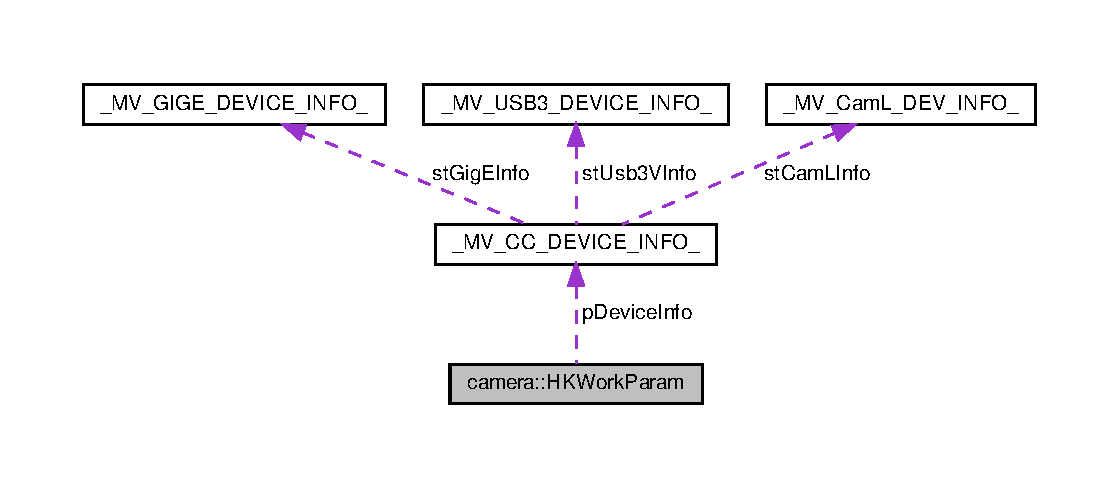
\includegraphics[width=350pt]{structcamera_1_1_h_k_work_param__coll__graph}
\end{center}
\end{figure}
\subsection*{Public 属性}
\begin{DoxyCompactItemize}
\item 
\mbox{\Hypertarget{structcamera_1_1_h_k_work_param_a1ad1b5015e364dea9367122b16f01727}\label{structcamera_1_1_h_k_work_param_a1ad1b5015e364dea9367122b16f01727}} 
void $\ast$ {\bfseries handle}
\item 
\mbox{\Hypertarget{structcamera_1_1_h_k_work_param_a57e297a0e197c238e14744a0743a5e0c}\label{structcamera_1_1_h_k_work_param_a57e297a0e197c238e14744a0743a5e0c}} 
\hyperlink{struct___m_v___c_c___d_e_v_i_c_e___i_n_f_o__}{M\+V\+\_\+\+C\+C\+\_\+\+D\+E\+V\+I\+C\+E\+\_\+\+I\+N\+FO} $\ast$ {\bfseries p\+Device\+Info}
\end{DoxyCompactItemize}


该结构体的文档由以下文件生成\+:\begin{DoxyCompactItemize}
\item 
camera/hikvision/src/hikvision\+\_\+camera.\+cpp\end{DoxyCompactItemize}

\hypertarget{class_l_o_g}{}\section{L\+O\+G类 参考}
\label{class_l_o_g}\index{L\+OG@{L\+OG}}
\subsection*{静态 Public 成员函数}
\begin{DoxyCompactItemize}
\item 
static void \hyperlink{class_l_o_g_a1b45763037b155a33161d976075ed095}{set\+Destination} (const std\+::string \&log\+Path)
\item 
static void \hyperlink{class_l_o_g_a439dbd171730d3ed670a92a58470fc52}{set\+Level} (const char $\ast$level)
\item 
static void \hyperlink{class_l_o_g_a291b1ef543ba201966bbda435483fceb}{close} ()
\item 
static void \hyperlink{class_l_o_g_a0912ae4707f37b1741caab70c763b29a}{info} (const char $\ast$log)
\item 
static void \hyperlink{class_l_o_g_a087b2e52961e2da0d3573d6520636af7}{info} (const std\+::string \&log)
\item 
static void \hyperlink{class_l_o_g_ab18febc5ce89c7f4868eb4fa28cf5eec}{debug} (const char $\ast$log)
\item 
static void \hyperlink{class_l_o_g_a90cb170f309538e4049a7da76a49809c}{debug} (const std\+::string \&log)
\item 
static void \hyperlink{class_l_o_g_a3ca4a93a22083c81ee039bcba71bdfa1}{error} (const char $\ast$log)
\item 
static void \hyperlink{class_l_o_g_aa295e0a02fca70f631d9074aa05cbf6c}{error} (const std\+::string \&log)
\item 
\mbox{\Hypertarget{class_l_o_g_a56e21057dae6d93137e494aa287ae96d}\label{class_l_o_g_a56e21057dae6d93137e494aa287ae96d}} 
static std\+::string {\bfseries tostring} (int i)
\item 
\mbox{\Hypertarget{class_l_o_g_a687072bfe75df90f7623946769452269}\label{class_l_o_g_a687072bfe75df90f7623946769452269}} 
static std\+::string {\bfseries tostring} (double i)
\item 
\mbox{\Hypertarget{class_l_o_g_a73e20af180c648251ea7a88269d1aedf}\label{class_l_o_g_a73e20af180c648251ea7a88269d1aedf}} 
static std\+::string {\bfseries tostring} (long i)
\item 
\mbox{\Hypertarget{class_l_o_g_a6afbd68da0a851352f23e33c72c0f88d}\label{class_l_o_g_a6afbd68da0a851352f23e33c72c0f88d}} 
static std\+::string {\bfseries tostring} (float i)
\item 
\mbox{\Hypertarget{class_l_o_g_a1342573c06dabaf882d21660b6cb8595}\label{class_l_o_g_a1342573c06dabaf882d21660b6cb8595}} 
static std\+::string {\bfseries tostring} (unsigned i)
\item 
\mbox{\Hypertarget{class_l_o_g_abc07f6597c14708770b9293ae0449ea7}\label{class_l_o_g_abc07f6597c14708770b9293ae0449ea7}} 
static std\+::string {\bfseries tostring} (bool i)
\item 
\mbox{\Hypertarget{class_l_o_g_a18839c11cbe91534fdf35e776b065b0a}\label{class_l_o_g_a18839c11cbe91534fdf35e776b065b0a}} 
static std\+::string {\bfseries tostring} (const char $\ast$i)
\end{DoxyCompactItemize}


\subsection{成员函数说明}
\mbox{\Hypertarget{class_l_o_g_a291b1ef543ba201966bbda435483fceb}\label{class_l_o_g_a291b1ef543ba201966bbda435483fceb}} 
\index{L\+OG@{L\+OG}!close@{close}}
\index{close@{close}!L\+OG@{L\+OG}}
\subsubsection{\texorpdfstring{close()}{close()}}
{\footnotesize\ttfamily static void L\+O\+G\+::close (\begin{DoxyParamCaption}{ }\end{DoxyParamCaption})\hspace{0.3cm}{\ttfamily [inline]}, {\ttfamily [static]}}

�ر���־ \mbox{\Hypertarget{class_l_o_g_ab18febc5ce89c7f4868eb4fa28cf5eec}\label{class_l_o_g_ab18febc5ce89c7f4868eb4fa28cf5eec}} 
\index{L\+OG@{L\+OG}!debug@{debug}}
\index{debug@{debug}!L\+OG@{L\+OG}}
\subsubsection{\texorpdfstring{debug()}{debug()}\hspace{0.1cm}{\footnotesize\ttfamily [1/2]}}
{\footnotesize\ttfamily static void L\+O\+G\+::debug (\begin{DoxyParamCaption}\item[{const char $\ast$}]{log }\end{DoxyParamCaption})\hspace{0.3cm}{\ttfamily [inline]}, {\ttfamily [static]}}

��ӡdebug��־ 
\begin{DoxyParams}{参数}
{\em log} & ��־���� \\
\hline
\end{DoxyParams}
\mbox{\Hypertarget{class_l_o_g_a90cb170f309538e4049a7da76a49809c}\label{class_l_o_g_a90cb170f309538e4049a7da76a49809c}} 
\index{L\+OG@{L\+OG}!debug@{debug}}
\index{debug@{debug}!L\+OG@{L\+OG}}
\subsubsection{\texorpdfstring{debug()}{debug()}\hspace{0.1cm}{\footnotesize\ttfamily [2/2]}}
{\footnotesize\ttfamily static void L\+O\+G\+::debug (\begin{DoxyParamCaption}\item[{const std\+::string \&}]{log }\end{DoxyParamCaption})\hspace{0.3cm}{\ttfamily [inline]}, {\ttfamily [static]}}

��ӡdebug��־ 
\begin{DoxyParams}{参数}
{\em log} & ��־���� \\
\hline
\end{DoxyParams}
\mbox{\Hypertarget{class_l_o_g_a3ca4a93a22083c81ee039bcba71bdfa1}\label{class_l_o_g_a3ca4a93a22083c81ee039bcba71bdfa1}} 
\index{L\+OG@{L\+OG}!error@{error}}
\index{error@{error}!L\+OG@{L\+OG}}
\subsubsection{\texorpdfstring{error()}{error()}\hspace{0.1cm}{\footnotesize\ttfamily [1/2]}}
{\footnotesize\ttfamily static void L\+O\+G\+::error (\begin{DoxyParamCaption}\item[{const char $\ast$}]{log }\end{DoxyParamCaption})\hspace{0.3cm}{\ttfamily [inline]}, {\ttfamily [static]}}

��ӡerror��־ 
\begin{DoxyParams}{参数}
{\em log} & ��־���� \\
\hline
\end{DoxyParams}
\mbox{\Hypertarget{class_l_o_g_aa295e0a02fca70f631d9074aa05cbf6c}\label{class_l_o_g_aa295e0a02fca70f631d9074aa05cbf6c}} 
\index{L\+OG@{L\+OG}!error@{error}}
\index{error@{error}!L\+OG@{L\+OG}}
\subsubsection{\texorpdfstring{error()}{error()}\hspace{0.1cm}{\footnotesize\ttfamily [2/2]}}
{\footnotesize\ttfamily static void L\+O\+G\+::error (\begin{DoxyParamCaption}\item[{const std\+::string \&}]{log }\end{DoxyParamCaption})\hspace{0.3cm}{\ttfamily [inline]}, {\ttfamily [static]}}

��ӡerror��־ 
\begin{DoxyParams}{参数}
{\em log} & ��־���� \\
\hline
\end{DoxyParams}
\mbox{\Hypertarget{class_l_o_g_a0912ae4707f37b1741caab70c763b29a}\label{class_l_o_g_a0912ae4707f37b1741caab70c763b29a}} 
\index{L\+OG@{L\+OG}!info@{info}}
\index{info@{info}!L\+OG@{L\+OG}}
\subsubsection{\texorpdfstring{info()}{info()}\hspace{0.1cm}{\footnotesize\ttfamily [1/2]}}
{\footnotesize\ttfamily static void L\+O\+G\+::info (\begin{DoxyParamCaption}\item[{const char $\ast$}]{log }\end{DoxyParamCaption})\hspace{0.3cm}{\ttfamily [inline]}, {\ttfamily [static]}}

��ӡinfo��־ 
\begin{DoxyParams}{参数}
{\em log} & ��־���� \\
\hline
\end{DoxyParams}
\mbox{\Hypertarget{class_l_o_g_a087b2e52961e2da0d3573d6520636af7}\label{class_l_o_g_a087b2e52961e2da0d3573d6520636af7}} 
\index{L\+OG@{L\+OG}!info@{info}}
\index{info@{info}!L\+OG@{L\+OG}}
\subsubsection{\texorpdfstring{info()}{info()}\hspace{0.1cm}{\footnotesize\ttfamily [2/2]}}
{\footnotesize\ttfamily static void L\+O\+G\+::info (\begin{DoxyParamCaption}\item[{const std\+::string \&}]{log }\end{DoxyParamCaption})\hspace{0.3cm}{\ttfamily [inline]}, {\ttfamily [static]}}

��ӡinfo��־ 
\begin{DoxyParams}{参数}
{\em log} & ��־���� \\
\hline
\end{DoxyParams}
\mbox{\Hypertarget{class_l_o_g_a1b45763037b155a33161d976075ed095}\label{class_l_o_g_a1b45763037b155a33161d976075ed095}} 
\index{L\+OG@{L\+OG}!set\+Destination@{set\+Destination}}
\index{set\+Destination@{set\+Destination}!L\+OG@{L\+OG}}
\subsubsection{\texorpdfstring{set\+Destination()}{setDestination()}}
{\footnotesize\ttfamily static void L\+O\+G\+::set\+Destination (\begin{DoxyParamCaption}\item[{const std\+::string \&}]{log\+Path }\end{DoxyParamCaption})\hspace{0.3cm}{\ttfamily [inline]}, {\ttfamily [static]}}

������־�洢λ�úͱ���ͼƬλ�� 
\begin{DoxyParams}{参数}
{\em log\+Path} & ��־�洢λ�� \\
\hline
{\em save\+Img\+Path} & ����ͼƬλ�� \\
\hline
\end{DoxyParams}
\mbox{\Hypertarget{class_l_o_g_a439dbd171730d3ed670a92a58470fc52}\label{class_l_o_g_a439dbd171730d3ed670a92a58470fc52}} 
\index{L\+OG@{L\+OG}!set\+Level@{set\+Level}}
\index{set\+Level@{set\+Level}!L\+OG@{L\+OG}}
\subsubsection{\texorpdfstring{set\+Level()}{setLevel()}}
{\footnotesize\ttfamily static void L\+O\+G\+::set\+Level (\begin{DoxyParamCaption}\item[{const char $\ast$}]{level }\end{DoxyParamCaption})\hspace{0.3cm}{\ttfamily [inline]}, {\ttfamily [static]}}

������־����ȱʡΪinfo����ѡdebug 
\begin{DoxyParams}{参数}
{\em level} & ��־���� \\
\hline
\end{DoxyParams}


该类的文档由以下文件生成\+:\begin{DoxyCompactItemize}
\item 
camera/hikvision/tool/include/C\+A\+M\+E\+R\+A\+\_\+\+L\+O\+G.\+h\end{DoxyCompactItemize}

\chapter{文件说明}
\hypertarget{main_8cpp}{}\section{main.\+cpp 文件参考}
\label{main_8cpp}\index{main.\+cpp@{main.\+cpp}}


This is a brief description.  


{\ttfamily \#include $<$iostream$>$}\newline
{\ttfamily \#include $<$opencv2/core/core.\+hpp$>$}\newline
{\ttfamily \#include $<$opencv2/highgui/highgui.\+hpp$>$}\newline
{\ttfamily \#include \char`\"{}inference.\+h\char`\"{}}\newline
{\ttfamily \#include \char`\"{}hikvision\+\_\+camera.\+h\char`\"{}}\newline
main.\+cpp 的引用(Include)关系图\+:\nopagebreak
\begin{figure}[H]
\begin{center}
\leavevmode
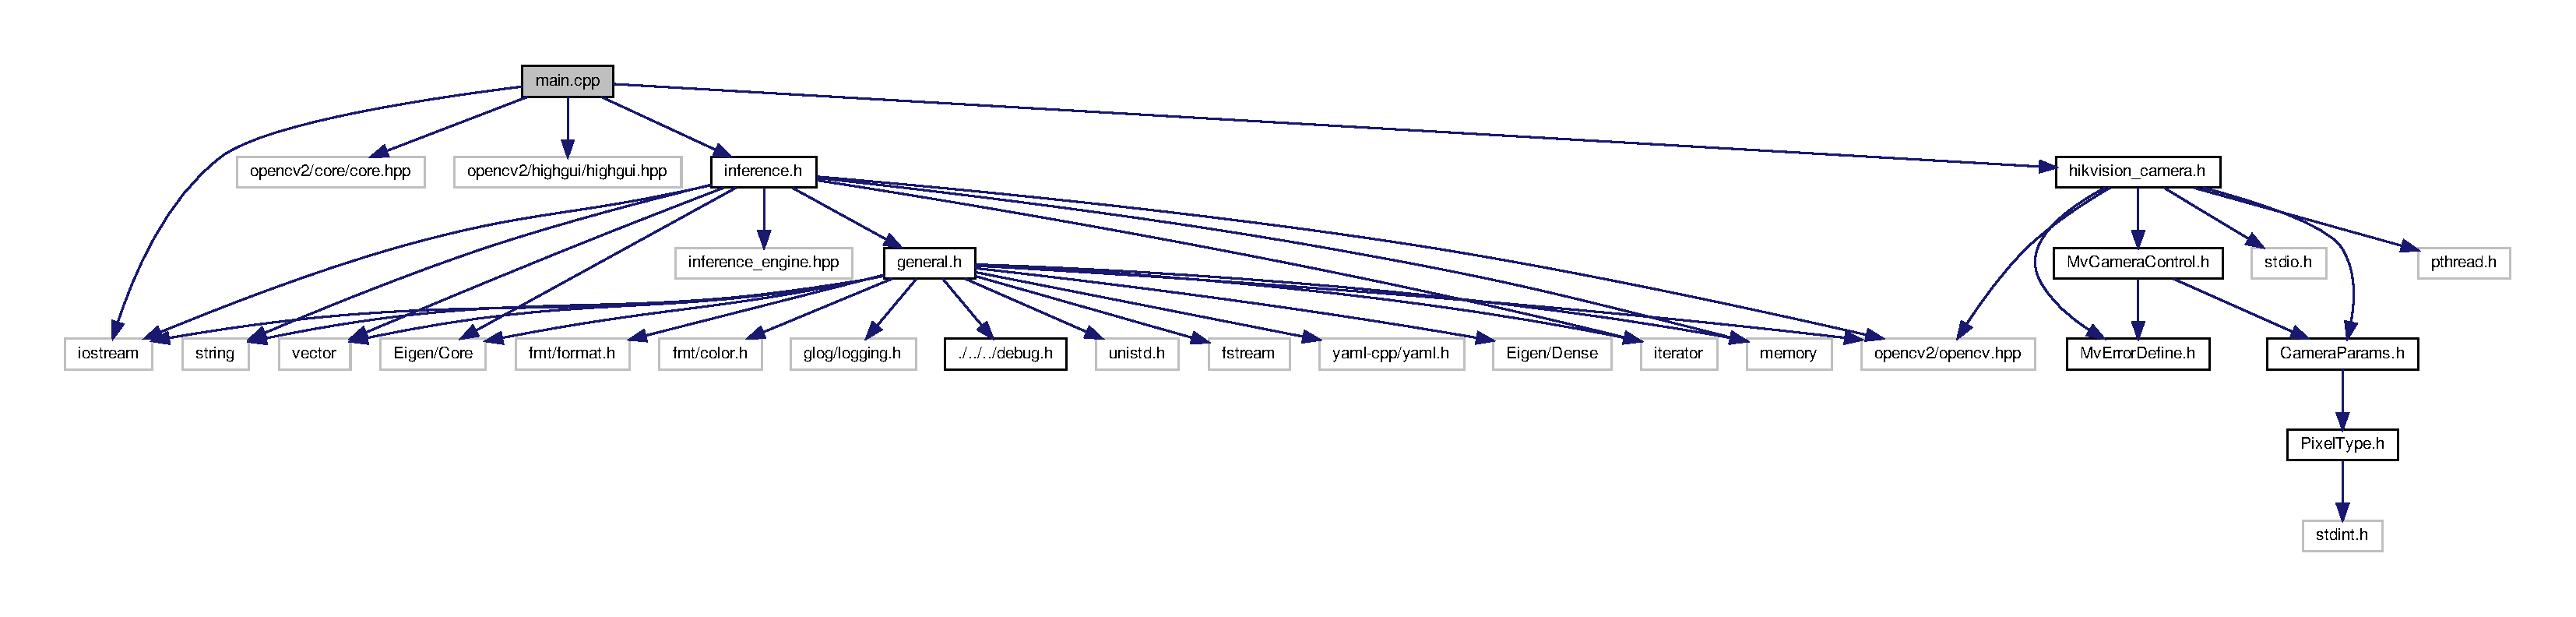
\includegraphics[width=350pt]{main_8cpp__incl}
\end{center}
\end{figure}
\subsection*{函数}
\begin{DoxyCompactItemize}
\item 
void \hyperlink{main_8cpp_a3b02b733a035cc05558426c0d12cb3ff}{display} (\hyperlink{struct_armor_object}{Armor\+Object})
\item 
int \hyperlink{main_8cpp_ae66f6b31b5ad750f1fe042a706a4e3d4}{main} ()
\end{DoxyCompactItemize}
\subsection*{变量}
\begin{DoxyCompactItemize}
\item 
\mbox{\Hypertarget{main_8cpp_a990d7b054e9e3bf406dca9afb6ee84ae}\label{main_8cpp_a990d7b054e9e3bf406dca9afb6ee84ae}} 
cv\+::\+Mat {\bfseries ori\+\_\+src}
\item 
\mbox{\Hypertarget{main_8cpp_a8e85f53775931ce972c464c2446ce3ec}\label{main_8cpp_a8e85f53775931ce972c464c2446ce3ec}} 
cv\+::\+Mat {\bfseries image2show}
\item 
\mbox{\Hypertarget{main_8cpp_a988c3306e17660881c1ae04a0e1fcf34}\label{main_8cpp_a988c3306e17660881c1ae04a0e1fcf34}} 
Video\+Capture {\bfseries capture}
\item 
\mbox{\Hypertarget{main_8cpp_a247f180a12f40713f0c428fc8ce59635}\label{main_8cpp_a247f180a12f40713f0c428fc8ce59635}} 
\hyperlink{class_armor_detector}{Armor\+Detector} {\bfseries detector}
\item 
\mbox{\Hypertarget{main_8cpp_a7eb08b64a155fdb3b17737a939e3e103}\label{main_8cpp_a7eb08b64a155fdb3b17737a939e3e103}} 
\hyperlink{classcamera_1_1_hik_camera}{Hik\+Camera} {\bfseries M\+V\+S\+\_\+cap}
\end{DoxyCompactItemize}


\subsection{详细描述}
This is a brief description. 

This is the detail description. \begin{DoxyAuthor}{作者}
tk 
\end{DoxyAuthor}
\begin{DoxyDate}{日期}
date 
\end{DoxyDate}
\begin{DoxyVersion}{版本}
A001 
\end{DoxyVersion}
\begin{DoxyParagraph}{Copyright (c)\+:}
S\+I-\/\+X\+U\+AN Robot\+Team 
\end{DoxyParagraph}
\begin{DoxyParagraph}{History\+:}
version\+: author, date, desc~\newline

\end{DoxyParagraph}


\subsection{函数说明}
\mbox{\Hypertarget{main_8cpp_a3b02b733a035cc05558426c0d12cb3ff}\label{main_8cpp_a3b02b733a035cc05558426c0d12cb3ff}} 
\index{main.\+cpp@{main.\+cpp}!display@{display}}
\index{display@{display}!main.\+cpp@{main.\+cpp}}
\subsubsection{\texorpdfstring{display()}{display()}}
{\footnotesize\ttfamily void display (\begin{DoxyParamCaption}\item[{\hyperlink{struct_armor_object}{Armor\+Object}}]{object }\end{DoxyParamCaption})}

This is a brief description. This is a detail description. 
\begin{DoxyParams}[1]{参数}
\mbox{\tt in}  & {\em in\+Arg\+Name} & input argument description. \\
\hline
\mbox{\tt out}  & {\em out\+Arg\+Name} & output argument description. \\
\hline
\end{DoxyParams}

\begin{DoxyRetVals}{返回值}
{\em OK} & 成功 \\
\hline
{\em E\+R\+R\+OR} & 错误 \\
\hline
\end{DoxyRetVals}
\begin{DoxyParagraph}{标识符}
保留 
\end{DoxyParagraph}
\begin{DoxyParagraph}{其它}
无 
\end{DoxyParagraph}
\begin{DoxyParagraph}{修改日志}
X\+X\+X于201\+X-\/\+X\+X-\/\+X\+X创建 
\end{DoxyParagraph}
\mbox{\Hypertarget{main_8cpp_ae66f6b31b5ad750f1fe042a706a4e3d4}\label{main_8cpp_ae66f6b31b5ad750f1fe042a706a4e3d4}} 
\index{main.\+cpp@{main.\+cpp}!main@{main}}
\index{main@{main}!main.\+cpp@{main.\+cpp}}
\subsubsection{\texorpdfstring{main()}{main()}}
{\footnotesize\ttfamily int main (\begin{DoxyParamCaption}{ }\end{DoxyParamCaption})}

This is a brief description. This is a detail description. 
\begin{DoxyParams}[1]{参数}
\mbox{\tt in}  & {\em in\+Arg\+Name} & input argument description. \\
\hline
\mbox{\tt out}  & {\em out\+Arg\+Name} & output argument description. \\
\hline
\end{DoxyParams}

\begin{DoxyRetVals}{返回值}
{\em OK} & 成功 \\
\hline
{\em E\+R\+R\+OR} & 错误 \\
\hline
\end{DoxyRetVals}
\begin{DoxyParagraph}{标识符}
保留 
\end{DoxyParagraph}
\begin{DoxyParagraph}{其它}
无 
\end{DoxyParagraph}
\begin{DoxyParagraph}{修改日志}
X\+X\+X于201\+X-\/\+X\+X-\/\+X\+X创建 
\end{DoxyParagraph}

%--- End generated contents ---

% Index
\backmatter
\newpage
\phantomsection
\clearemptydoublepage
\addcontentsline{toc}{chapter}{索引}
\printindex

\end{document}
